%%
%% This is file `sample-acmsmall-conf.tex',
%% generated with the docstrip utility.
%%
%% The original source files were:
%%
%% samples.dtx  (with options: `acmsmall-conf')
%% 
%% IMPORTANT NOTICE:
%% 
%% For the copyright see the source file.
%% 
%% Any modified versions of this file must be renamed
%% with new filenames distinct from sample-acmsmall-conf.tex.
%% 
%% For distribution of the original source see the terms
%% for copying and modification in the file samples.dtx.
%% 
%% This generated file may be distributed as long as the
%% original source files, as listed above, are part of the
%% same distribution. (The sources need not necessarily be
%% in the same archive or directory.)
%%
%%
%% Commands for TeXCount
%TC:macro \cite [option:text,text]
%TC:macro \citep [option:text,text]
%TC:macro \citet [option:text,text]
%TC:envir table 0 1
%TC:envir table* 0 1
%TC:envir tabular [ignore] word
%TC:envir displaymath 0 word
%TC:envir math 0 word
%TC:envir comment 0 0
%%
%%
%% The first command in your LaTeX source must be the \documentclass
%% command.
%%
%% For submission and review of your manuscript please change the
%% command to \documentclass[manuscript, screen, review]{acmart}.
%%
%% When submitting camera ready or to TAPS, please change the command
%% to \documentclass[sigconf]{acmart} or whichever template is required
%% for your publication.
%%
%%
%\documentclass[sigconf,anonymous]{acmart}
% https://conf.researchr.org/track/esem-2024/esem-2024-technical-track
% All submissions must be written in English and must be submitted via EasyChair
% in the PDF format, and they must be formatted according to the ACM proceedings
% template, which can be found at ACM Proceedings Template (https://www.acm.org/publications/proceedings-template) or in Overleaf at https://www.overleaf.com/gallery/tagged/acm).
\PassOptionsToPackage{table}{xcolor}
\documentclass[sigconf,nonacm]{acmart}
%\acmConference[ESEC/FSE 2023]{The 31st ACM Joint European Software Engineering Conference and Symposium on the Foundations of Software Engineering}{11 - 17 November, 2023}{San Francisco, USA}
\hypersetup{
   colorlinks=true,
  pdfborder={0 0 0},
}
%%
%% \BibTeX command to typeset BibTeX logo in the docs
\AtBeginDocument{%
  \providecommand\BibTeX{{%
    Bib\TeX}}}

%SPACE \setlength{\parskip}{0cm}
%SPACE \setlength{\parindent}{1em}
\usepackage{paralist}
%XXXXXXXXXXXXXX
\newcommand{\mytitle}{An Empirical Evaluation of Frequency-Based Statistical Models for Estimating Killable Mutants}

% ALESSIO: A Large Empirical Evaluation of Frequency-Based Statistical Models for Estimating Killable Mutants
% ALESSIO: Empirically Evaluating Frequency-Based Statistical Models for Estimating Killable Mutants
% ALESSIO: A Large Empirical Evaluation of Frequency-Based Statistical Models applied to Mutation Testing

% ALESSIO: Check whether we use "Frequency-Based Statistical Models" in the paper or something else (e.g., "Bio-Inspired Estimators")

%Estimating Equivalent Mutants: Are we there yet?}
%\newcommand{\mytitle}{Estimating Equivalent Mutants: Are we there yet?}
%\usepackage{hyperref}
%\usepackage{xcolor}
\definecolor{rltred}{rgb}{0.5,0,0}
\definecolor{rltgreen}{rgb}{0,0.5,0}
\definecolor{rltblue}{rgb}{0,0,0.5}
\hypersetup{
colorlinks=true,
urlcolor=rltblue, % was rltblue
linkcolor=rltblue,
citecolor=rltblue,
filecolor=rltblue,         % color of file links
pdftitle={\mytitle}
}
\newif\ifdraft\drafttrue
\newif\iflong\longfalse

\definecolor{eclipseBlue}{RGB}{42,0.0,255}
\definecolor{eclipseGreen}{RGB}{63,127,95}
\definecolor{eclipsePurple}{RGB}{127,0,85}
\definecolor{darkgreen}{RGB}{1,50,32}

\usepackage[procnames]{listings}
\lstdefinestyle{python}
{
    breaklines=false,
    basicstyle=\footnotesize\ttfamily,
    numberblanklines=false,
    language=python,
    tabsize=2,
    commentstyle=\color{eclipseGreen},
    keywordstyle=\bfseries\color{eclipsePurple},
    stringstyle=\color{eclipseBlue},
    procnamestyle=\bfseries\color{black},
    procnamekeys={def},
    columns=flexible,
    identifierstyle=
}
\usepackage{tcolorbox}
\usepackage{amsfonts}

\definecolor{codegreen}{rgb}{0,0.6,0}
\definecolor{codegray}{rgb}{0.5,0.5,0.5}
\definecolor{codepurple}{rgb}{0.58,0,0.82}
\definecolor{codeorange}{rgb}{1,0.5,0}
\definecolor{backcolour}{rgb}{0.95,0.95,0.92}

\lstdefinestyle{mystyle}{
    % backgroundcolor=\color{backcolour},
    commentstyle=\color{codegreen},
    keywordstyle=\color{magenta},
    numberstyle=\tiny\color{codegray},
    stringstyle=\color{codepurple},
    basicstyle=\linespread{0.8}\ttfamily,
    breakatwhitespace=false,
    breaklines=true,
    captionpos=b,
    keepspaces=true,
    numbers=left,
    numbersep=5pt,
    showspaces=false,
    showstringspaces=false,
    showtabs=false,
    tabsize=2
}

\lstset{style=mystyle}

\definecolor{cgroundtruth}{RGB}{163,124,194}
\definecolor{cmethod}{RGB}{0,108,168}
\definecolor{cclass}{RGB}{219,36,42}

% The name of our central contribution, with variations
\usepackage{xspace}

%%%%
%
%
% How Many estimators do we consider?
%
%
%%%%
\newcommand{\estimatorCount}{twelve\xspace}
\newcommand{\projectCount}{ten\xspace}
\newcommand{\mutantCount}{110595\xspace}

\newcommand{\rA}{\textsc{R$_\text{A}$}\xspace}
\newcommand{\rB}{\textsc{R$_\text{B}$}\xspace}
\newcommand{\rC}{\textsc{R$_\text{C}$}\xspace}

\newcommand{\ICEallrare}{ICE-k0\xspace}
\newcommand{\Zelterman}{Zelterman\xspace}
\newcommand{\ChaoBunge}{Chao-Bunge\xspace}
\newcommand{\Jackknife}{Jackknife\xspace}
\newcommand{\Chao}{Chao\xspace}
%\newcommand{\Chaobiascorrected}{Chao-bc\xspace}
\newcommand{\improvedChao}{iChao\xspace}
\newcommand{\ICE}{ICE\xspace}
\newcommand{\improvedICE}{ICE-1\xspace}
\newcommand{\Unpmle}{UNPMLE\xspace}
\newcommand{\Bootstrap}{Bootstrap\xspace}
\newcommand{\Pnpmle}{PNPMLE\xspace}
\newcommand{\PCG}{PCG\xspace}

\newcommand{\chao}{$\hat{S}_\textit{Chao}$\xspace}

\newcounter{todocounter}
\newcommand{\todo}[1]{\marginpar{$|$}\textcolor{red}{\stepcounter{todocounter}\footnote[\thetodocounter]{\textcolor{red}{\textbf{TODO }}\textit{#1}}}}
\newcommand{\repl}[2]{\textcolor{red}{\textbf{REPLACE }\st{#1} \textit{#2}}}     
\newcommand{\rem}[1]{\textcolor{red}{\textbf{REMOVED }\st{#1}}}                  
                                                                                 
\newcommand{\done}[1]{\textcolor{green}{\stepcounter{todocounter}\endnote[\thetodocounter]{\textbf{DONE }\textit{#1}}}}

\InputIfFileExists{SUBMIT}{
\renewcommand{\todo}[1]{}
\renewcommand{\done}[1]{}
\renewcommand{\rem}[1]{}
}{}

\newcommand{\Randoop}{\textsc{Randoop}\xspace}
\newcommand{\Evosuite}{\textsc{EvoSuite}\xspace}
\newcommand{\original}{\textsc{Original}\xspace}
\newcommand{\PIT}{\textsc{PIT}\xspace}

\newcommand{\EvosuiteRandom}{\textsc{Random}\xspace}
%\newcommand{\EvosuiteStd}{\textsc{Evosuite-Standard}\xspace}
\newcommand{\EvosuiteDynamosa}{\textsc{DynaMOSA}\xspace}

\usepackage{cleveref}

%XXXXXXXXXXXXXX
\usepackage{adjustbox}
%\usepackage{graphicx}
\usepackage{pgf,tikz}

\usepackage{xcolor}
%\newcommand*\circled[1]{\tikz[baseline=(char.base)]{
            %\node[shape=circle,fill,inner sep=2pt] (char) {\textcolor{white}{#1}};}}
\newcommand*\circled[1]{\tikz[baseline=(char.base)]{
            \node[shape=circle,draw,inner sep=2pt] (char) {#1};}}
% \newcommand{\RQA}{RQ1\xspace} %\circled{A}\xspace}
% \newcommand{\RQB}{RQ2\xspace} %\circled{B}\xspace}
% \newcommand{\RQC}{RQ3\xspace} %\circled{C}\xspace}
% \newcommand{\RQD}{RQ4\xspace} %\circled{D}\xspace}
\newcommand{\RQA}{\circled{1}\xspace}
\newcommand{\RQB}{\circled{2}\xspace}
\newcommand{\RQC}{\circled{3}\xspace}
\newcommand{\RQD}{\circled{4}\xspace}


\newcommand{\RQAx}{%
\begin{description}\item[\RQA]\textbf{What is the accuracy of frequency-based estimators in predicting killable mutants?}\end{description}}

\newcommand{\RQBx}{%
\begin{description}\item[\RQB]\textbf{Are frequency-based estimators affected by sampling strategies?}\end{description}}

\newcommand{\RQCx}{%
\begin{description}\item[\RQC] \textbf{Are frequency-based estimators affected by sampling units?}\end{description}}




\usepackage{endnotes}
\usepackage{pifont}
\usepackage{widetable}
\usepackage{mathtools}
\DeclarePairedDelimiter{\ceil}{\lceil}{\rceil}
\usepackage{doi}
%\usepackage{microtype}
\usepackage{forest}
%\usepackage{comment}
\usepackage{footmisc}
\usepackage[noend]{algpseudocode}
\usepackage{algorithm}
\usepackage{algorithmicx}
\usepackage{epstopdf}
\usepackage{textcomp}
\usepackage{boxedminipage}
\usepackage{float}
\usepackage{soul}
\usepackage{alltt}

%\usepackage{mdwtab}
\usepackage{syntax}
\usepackage{lstautogobble}
\usepackage{qtree}

% \Crefname{figure}{Fig.}{Figs.}
% \Crefname{equation}{Eqn.}{Eqns.}
% \crefname{section}{Section}{Sections}
% \Crefname{subsection}{Section}{Sections}
% \Crefname{Algorithm}{Alg.}{Algs.}

\usepackage{subcaption}
\usepackage{multirow}

%\usepackage{balance}
\usepackage[inline]{enumitem}
\usetikzlibrary{shapes.misc, positioning}

\usepackage{url}
%\usepackage{booktabs}

\usepackage{amsmath}
%\usepackage{amssymb}

\newcommand{\B}[1]{\textbf{#1}}

\newcommand{\Coreutils}{UNIX command line utilities\xspace}

\algblockdefx[switch]{Switch}{EndSwitch}%
[1]{\textbf{switch} #1}%
{}%
\algloopdefx{Case}[1]{\textbf{case} #1:}%
\algdef{SE}[DOWHILE]{Do}{doWhile}{\algorithmicdo}[1]{\algorithmicwhile\ #1}%

\algnewcommand\RETURN{\State \algorithmicreturn}%

\usepackage{contour}
\usepackage[normalem]{ulem}

\setlength{\ULdepth}{1.8pt}
\contourlength{0.8pt}

\newcommand{\myuline}[1]{%
  \uline{\phantom{#1}}%
  \llap{\contour{white}{#1}}%
}

\newenvironment{result}%
{\medskip
\noindent
\let\emph=\textbf\begin{center}
\begin{boxedminipage}{\columnwidth}\begin{center}\em}%
{\end{center}\end{boxedminipage}\end{center}%
\medskip
}

\def\term#1{\texttt{'\textbf{#1}'}}
\newcommand{\termC}[2]{\texttt{'\textbf{\color{#2}#1}'}}
\def\nonterm#1{\textnormal{\emph{#1}}}
\def\regex#1{\texttt{{\color{blue}/}#1{\color{blue}/}}}
\def\expandsto{\(\rightarrow{}\)}

\definecolor{nontermcolor}{rgb}{0.4, 0.05, 0.0} % dark orange
\definecolor{absnontermcolor}{rgb}{0.4, 0.5, 0.0} % light green
\definecolor{evokcolor}{rgb}{0.8, 0.05, 0.1}    % orange
\definecolor{incorrectcolor}{rgb}{0.5, 0.0, 0.13}
\definecolor{incompletecolor}{rgb}{0.0, 0.0, 0.55}
\definecolor{validcolor}{rgb}{0.33, 0.42, 0.18} %  {0.0, 0.28, 0.67}
\definecolor{retcolor}{rgb}{0.65, 0.16, 0.16}
\definecolor{ipatterncolor}{rgb}{0.0, 0.5, 0.4} % cyan?
\definecolor{termcolor}{rgb}{0.0, 0.05, 0.4}    % dark blue
\definecolor{regexcolor}{rgb}{0.1, 0.3, 0.1}    % dark green

\def\term#1{\texttt{\color{termcolor}'\textbf{#1}'}}
\def\nonterm#1{{\color{nontermcolor}$\langle$\textnormal{\emph{#1}}$\rangle$}}
\def\absnonterm#1{{\color{absnontermcolor}$\langle$\textnormal{\emph{#1}}$\rangle$}}
\def\evoknt#1{{\color{evokcolor}$\langle$\textnormal{\emph{#1}}$\rangle$}}
\def\ipattern#1{\color{ipatterncolor}#1}
\def\regex#1{\texttt{\color{regexcolor}/#1/}}
\def\expandsto{::=}

\newcommand{\cmark}{\ding{51}}%
\newcommand{\xmark}{\ding{55}}%
\newcommand{\dmark}{\ding{108}}%
\def\ret#1{\texttt{\color{retcolor}\textbf{\small#1}}}

\def\Rincomplete{\texttt{\color{incompletecolor}\textbf{$\vartriangleright$}}\xspace}
\def\Rincorrect{\texttt{\color{incorrectcolor}\textbf{$\ntriangleright$}}\xspace}
\def\Rvalid{\texttt{\color{validcolor}\textbf{$\blacksquare$}}\xspace}

\renewcommand{\ulitleft}{\normalfont\ttfamily}
\renewcommand{\litleft}{\bgroup\color{termcolor}`\ulitleft}
\renewcommand{\litright}{\ulitright'\egroup}

\renewcommand{\syntleft}{\bgroup\color{nontermcolor}$\langle$\normalfont\itshape}
\renewcommand{\syntright}{$\rangle$\egroup}

\grammarparsep 3pt plus 1pt minus 1pt

\newenvironment{densegrammar}{%
\begin{small}
\begin{grammar}%
}%
{%
\end{grammar}%
\end{small}%
}
\newenvironment{Grammar}%
{\begin{itemize}\item[]\begin{densegrammar}}%
{\end{densegrammar}\end{itemize}}%

\def\instrumentationless{instrumentationless\xspace}
\def\Pyparsing{\emph{Pyparsing}\xspace}
\def\Gparsing{\emph{General Parsers}\xspace}
\def\|#1|{\textit{#1}}
\def\<#1>{\texttt{#1}}
%\def\[[#1\]]{\texttt{#1}} % better?

% \newcounter{todocounter}
% \newcommand{\todo}[1]{\marginpar{$|$}\textcolor{red}{\stepcounter{todocounter}\footnote[\thetodocounter]{\textcolor{red}{\textbf{TODO }}\textit{#1}}}}
% \newcommand{\repl}[2]{\textcolor{red}{\textbf{REPLACE }\st{#1} \textit{#2}}}
% \newcommand{\rem}[1]{\textcolor{red}{\textbf{REMOVED }\st{#1}}}
% 
% \newcommand{\done}[1]{\textcolor{green}{\stepcounter{todocounter}\endnote[\thetodocounter]{\textbf{DONE }\textit{#1}}}}

\IfFileExists{SUBMIT}{
\renewcommand{\todo}[1]{}
\renewcommand{\done}[1]{}
\renewcommand{\rem}[1]{}
\renewcommand{\theendnotes}{}
}

\definecolor{eclipseBlue}{RGB}{42,0.0,255}
\definecolor{eclipseGreen}{RGB}{63,127,95}
\definecolor{eclipsePurple}{RGB}{127,0,85}

\newcommand{\decoder}{\textsc{Decoder}\xspace}
\newcommand{\decoderNS}{\textsc{Decoder}\xspace}
\newcommand{\pFuzzer}{pFuzzer\xspace}
\newcommand{\pFuzzerNS}{pFuzzer\xspace}
\newcommand{\lFuzzer}{lFuzzer\xspace}
\newcommand{\lFuzzerNS}{lFuzzer\xspace}

\definecolor{eclipseBlue}{RGB}{42,0.0,255}
\definecolor{eclipseGreen}{RGB}{63,127,95}
\definecolor{eclipsePurple}{RGB}{127,0,85}

%\usepackage[procnames]{listings}
\lstdefinestyle{asm}
{
    basicstyle=\footnotesize\ttfamily,
    numberblanklines=false,
    language=assembly,
    tabsize=2,
    commentstyle=\color{eclipseGreen},
    keywordstyle=\bfseries\color{eclipsePurple},
    stringstyle=\color{eclipseBlue},
    procnamestyle=\bfseries\color{black},
    numbers=none,
    procnamekeys={},
    columns=flexible,
    xleftmargin=3mm,
    framexleftmargin=1mm,
    identifierstyle=
}
\lstdefinestyle{python}
{
    basicstyle=\footnotesize\ttfamily,
    numberblanklines=false,
    language=python,
    tabsize=2,
    commentstyle=\color{eclipseGreen},
    keywordstyle=\bfseries\color{eclipsePurple},
    stringstyle=\color{eclipseBlue},
    procnamestyle=\bfseries\color{black},
    morekeywords={where,match,case},            % if you want to add more keywords to the set
    numbers=left,
    procnamekeys={def},
    columns=flexible,
    xleftmargin=3mm,
    framexleftmargin=1mm,
    identifierstyle=
}

\definecolor{codegreen}{rgb}{0,0.6,0}
\definecolor{codegray}{rgb}{0.5,0.5,0.5}
\definecolor{codepurple}{rgb}{0.58,0,0.82}
\definecolor{backcolour}{rgb}{0.95,0.95,0.92}

\lstdefinestyle{mystyle}{
    % backgroundcolor=\color{backcolour},
    basicstyle=\footnotesize\ttfamily,
    commentstyle=\color{codegreen},
    keywordstyle=\color{eclipsePurple},
    escapeinside={(*}{*)},          % if you want to add LaTeX within your code
    %numberstyle=\tiny\color{codegray},
    stringstyle=\color{codepurple},
    %basicstyle=\linespread{0.8}\ttfamily,
    breakatwhitespace=false,
    breaklines=true,
    captionpos=b,
    keepspaces=true,
    %numbers=left,
    %numbersep=5pt,
    %procnamestyle=\bfseries\color{black},
    %procnamekeys={where},
    morekeywords={where},            % if you want to add more keywords to the set
    showspaces=false,
    showstringspaces=false,
    showtabs=false,
    tabsize=2,
    deletekeywords={expected},
    morestring=[b]' % defines that strings are enclosed in quotes
}

\lstset{style=mystyle}

\newcommand{\pdtg}{parser-directed fuzzing\xspace}
\newcommand{\Pdtg}{Parser-directed fuzzing\xspace}
\newcommand{\pdtgN}{\textsc{pFuzzer}\xspace}
\newcommand{\KLEE}{KLEE\xspace}
\newcommand{\AFL}{AFL\xspace}
\newcommand{\AFLp}{AFL++\xspace}
\newcommand{\AFLplain}{AFL (\<-n>)\xspace}
\newcommand{\AFLW}{AFL with Waypoints\xspace}

\algblockdefx[switch]{Switch}{EndSwitch}%
[1]{\textbf{switch} #1}%
{}%
\algloopdefx{Case}[1]{\textbf{case} #1:}%
\algdef{SE}[DOWHILE]{Do}{doWhile}{\algorithmicdo}[1]{\algorithmicwhile\ #1}%

\newcommand{\json}{\textsc{json}\xspace}
\newcommand{\csv}{\textsc{csv}\xspace}
\newcommand{\ini}{\textsc{ini}\xspace}
\newcommand{\tinyc}{\textsc{tinyC}\xspace}
\newcommand{\mjs}{\textsc{mjs}\xspace}
\newcommand{\SC}{Statement Coverage\xspace}
\newcommand{\BC}{Branch Coverage\xspace}
\def\BibTeX{{\rm B\kern-.05em{\sc i\kern-.025em b}\kern-.08em
    T\kern-.1667em\lower.7ex\hbox{E}\kern-.125emX}}
\captionsetup{skip=7pt}
%% Rights management information.  This information is sent to you
%% when you complete the rights form.  These commands have SAMPLE
%% values in them; it is your responsibility as an author to replace
%% the commands and values with those provided to you when you
%% complete the rights form.
%\setcopyright{acmcopyright}
%\copyrightyear{2018}
%\acmYear{2018}
%\acmDOI{XXXXXXX.XXXXXXX}
\copyrightyear{2024}
\acmYear{2024}
\setcopyright{acmlicensed}\acmConference[ESEM '24]{Proceedings of the 18th ACM / IEEE International Symposium on Empirical Software Engineering and Measurement}{October 24--25, 2024}{Barcelona, Spain}
\acmBooktitle{Proceedings of the 18th ACM / IEEE International Symposium on Empirical Software Engineering and Measurement (ESEM '24), October 24--25, 2024, Barcelona, Spain}
\acmDOI{10.1145/3674805.3686669}
\acmISBN{979-8-4007-1047-6/24/10}
%% These commands are for a PROCEEDINGS abstract or paper.
%\acmConference[Conference acronym 'XX]{Make sure to enter the correct
%  conference title from your rights confirmation emai}{June 03--05,
%  2018}{Woodstock, NY}
%%
%%  Uncomment \acmBooktitle if the title of the proceedings is different
%%  from ``Proceedings of ...''!
%%
%%\acmBooktitle{Woodstock '18: ACM Symposium on Neural Gaze Detection,
%%  June 03--05, 2018, Woodstock, NY}
%\acmPrice{15.00}
%\acmISBN{978-1-4503-XXXX-X/18/06}

%%
%% Submission ID.
%% Use this when submitting an article to a sponsored event. You'll
%% receive a unique submission ID from the organizers
%% of the event, and this ID should be used as the parameter to this command.
%%\acmSubmissionID{123-A56-BU3}

%%
%% For managing citations, it is recommended to use bibliography
%% files in BibTeX format.
%%
%% You can then either use BibTeX with the ACM-Reference-Format style,
%% or BibLaTeX with the acmnumeric or acmauthoryear sytles, that include
%% support for advanced citation of software artefact from the
%% biblatex-software package, also separately available on CTAN.
%%
%% Look at the sample-*-biblatex.tex files for templates showcasing
%% the biblatex styles.
%%
%\usepackage[style=ACM-Reference-Format,backend=bibtex,sorting=none]{biblatex}
%%
%% The majority of ACM publications use numbered citations and
%% references.  The command \citestyle{authoryear} switches to the
%% "author year" style.
%%
%% If you are preparing content for an event
%% sponsored by ACM SIGGRAPH, you must use the "author year" style of
%% citations and references.
%% Uncommenting
%% the next command will enable that style.
%%\citestyle{acmauthoryear}
\author{Konstantin Kuznetsov}
\authornote{Both authors contributed equally to the paper}
\affiliation{\institution{CISPA}\country{Germany}}
\email{konstantin.kuznetsov@cispa.de}
\author{Alessio Gambi}
\authornotemark[1]
\affiliation{\institution{Fachhochschule Kärnten}\country{Austria}}
\email{alessio.gambi@fh-kerns.ac.at}
\author{Saikrishna Dhiddi}
\affiliation{\institution{University of Passau}\country{Germany}}
\email{dhiddi@ads.uni-passau.de}
\author{Julia Hess}
\affiliation{\institution{Saarland University}\country{Germany}}
\email{s9jahess@stud.uni-saarland.de}
\author{Rahul Gopinath}
\affiliation{\institution{University of Sydney}\country{Australia}}
\email{rahul.gopinath@sydney.edu.au}

%%
%% end of the preamble, start of the body of the document source.
\begin{document}

%%
%% The "title" command has an optional parameter,
%% allowing the author to define a "short title" to be used in page headers.
\title{\mytitle}

%%
%% The "author" command and its associated commands are used to define
%% the authors and their affiliations.
%% Of note is the shared affiliation of the first two authors, and the
%% "authornote" and "authornotemark" commands
%% used to denote shared contribution to the research.

%\author{Ben Trovato}
%\authornote{Both authors contributed equally to this research.}
%\email{trovato@corporation.com}
%\orcid{1234-5678-9012}
%\author{G.K.M. Tobin}
%\authornotemark[1]
%\email{webmaster@marysville-ohio.com}
%\affiliation{%
%  \institution{Institute for Clarity in Documentation}
%  \streetaddress{P.O. Box 1212}
%  \city{Dublin}
%  \state{Ohio}
%  \country{USA}
%  \postcode{43017-6221}
%}
%
%\author{Lars Th{\o}rv{\"a}ld}
%\affiliation{%
%  \institution{The Th{\o}rv{\"a}ld Group}
%  \streetaddress{1 Th{\o}rv{\"a}ld Circle}
%  \city{Hekla}
%  \country{Iceland}}
%\email{larst@affiliation.org}
%
%\author{Valerie B\'eranger}
%\affiliation{%
%  \institution{Inria Paris-Rocquencourt}
%  \city{Rocquencourt}
%  \country{France}
%}
%
%\author{Aparna Patel}
%\affiliation{%
% \institution{Rajiv Gandhi University}
% \streetaddress{Rono-Hills}
% \city{Doimukh}
% \state{Arunachal Pradesh}
% \country{India}}
%
%\author{Huifen Chan}
%\affiliation{%
%  \institution{Tsinghua University}
%  \streetaddress{30 Shuangqing Rd}
%  \city{Haidian Qu}
%  \state{Beijing Shi}
%  \country{China}}

%\author{Charles Palmer}
%\affiliation{%
%  \institution{Palmer Research Laboratories}
%  \streetaddress{8600 Datapoint Drive}
%  \city{San Antonio}
%  \state{Texas}
%  \country{USA}
%  \postcode{78229}}
%\email{cpalmer@prl.com}
%
%\author{John Smith}
%\affiliation{%
%  \institution{The Th{\o}rv{\"a}ld Group}
%  \streetaddress{1 Th{\o}rv{\"a}ld Circle}
%  \city{Hekla}
%  \country{Iceland}}
%\email{jsmith@affiliation.org}
%
%\author{Julius P. Kumquat}
%\affiliation{%
%  \institution{The Kumquat Consortium}
%  \city{New York}
%  \country{USA}}
%\email{jpkumquat@consortium.net}

%%
%% By default, the full list of authors will be used in the page
%% headers. Often, this list is too long, and will overlap
%% other information printed in the page headers. This command allows
%% the author to define a more concise list
%% of authors' names for this purpose.
%\renewcommand{\shortauthors}{Trovato et al.}

%%
%% The abstract is a short summary of the work to be presented in the
%% article.
\begin{abstract}
  % Background, Aims, Method, Results, and Conclusions
\noindent\textbf{Background.}
Mutation analysis is the premier technique for evaluating test suite
quality estimating residual software defects. However, the reliability of 
mutation analysis is hampered by \emph{equivalent mutants} which
are undetectable by test cases.
Reliably detecting and eliminating killable mutants is difficult
as it is highly program and location dependent. Statistical estimation of
killable mutants seems to be a promising approach to tackle this problem.\\
\noindent\textbf{Aims.}
Frequency-based species estimation methods
have been proposed as a solution for several related problems in software
testing.
%While promising, there has been no comprehensive study on whether
%such frequency-based species estimation methods can
%deliver an accurate estimate for killable mutants.
This paper investigates whether such frequency-based estimation methods
can accurately estimate the number of killable mutants.\\
\noindent\textbf{Method.}
We conducted a large-scale empirical study
on the ability of \estimatorCount widely known frequency-based
estimators to predict the number of killable mutants in
\projectCount mature software projects.\\
\noindent\textbf{Result.}
Our investigation finds limited or no evidence that any of the statistical
estimators are able to consistently predict the number of killable mutants in
projects evaluated.\\
\noindent\textbf{Conclusion.}
We found that the investigated estimators lack sufficient
predictive power and cannot produce reliable and useful estimates of killable
mutants. However, we found that the \emph{bootstrap} was the
best performing%, and most promising 
method out of all methods considered.
\end{abstract}

%%
%% The code below is generated by the tool at http://dl.acm.org/ccs.cfm.
%% Please copy and paste the code instead of the example below.
%%
%\begin{CCSXML}
%<ccs2012>
%<concept>
%<concept_id>10010520.10010553.10010562</concept_id>
%<concept_desc>Computer systems organization~Embedded systems</concept_desc>
%<concept_significance>500</concept_significance>
%</concept>
%<concept>
%<concept_id>10010520.10010575.10010755</concept_id>
%<concept_desc>Computer systems organization~Redundancy</concept_desc>
%<concept_significance>300</concept_significance>
%</concept>
%<concept>
%<concept_id>10010520.10010553.10010554</concept_id>
%<concept_desc>Computer systems organization~Robotics</concept_desc>
%<concept_significance>100</concept_significance>
%</concept>
%<concept>
%<concept_id>10003033.10003083.10003095</concept_id>
%<concept_desc>Networks~Network reliability</concept_desc>
%<concept_significance>100</concept_significance>
%</concept>
%</ccs2012>
%\end{CCSXML}
%
%\ccsdesc[500]{Computer systems organization~Embedded systems}
%\ccsdesc[300]{Computer systems organization~Redundancy}
%\ccsdesc{Computer systems organization~Robotics}
%\ccsdesc[100]{Networks~Network reliability}

%%
%% Keywords. The author(s) should pick words that accurately describe
%% the work being presented. Separate the keywords with commas.
%\keywords{mutation analysis, equivalent mutants, residual risk}
%% A "teaser" image appears between the author and affiliation
%% information and the body of the document, and typically spans the
%% page.

%\received{20 February 2007}
%\received[revised]{12 March 2009}
%\received[accepted]{5 June 2009}

%%
%% This command processes the author and affiliation and title
%% information and builds the first part of the formatted document.
\settopmatter{printacmref=false}

\maketitle

%XXXXXXXXXXXXXXXXXXXXXX
\section{Introduction}
Mutation analysis is the premier means of assessing the quality of
software test suites in preventing defects~\cite{papadakis2019mutation},
and estimating residual risk~\cite{horgan1996software}.
Mutation analysis involves
generating mutants \emph{exhaustively} and evaluating them against the test suite under consideration.
(\Cref{fig:working-example}-right).
%
Mutants are copies of the original code (\Cref{fig:working-example}-left) in which artificial code %simple, 
\emph{mutations} that share strong similarities with real faults are inserted (\Cref{fig:working-example-mutants})~\cite{daran1996software,just2014are,andrews2005is,andrews2006using}.

\begin{figure}[t]
\begin{minipage}{.45\columnwidth}  %listing bloc will have 50% of the line width 
%\lstset{linewidth = 4cm, breaklines=true} %set your listing lines widths, and set breaklines to true
\begin{lstlisting}[style=python]
def determinant(a,b,c,d):
  ad = a * d
  bc = b * c
  return ad - bc
\end{lstlisting}
\end{minipage}
\hfill
\begin{minipage}{0.5\columnwidth} %figure will have the remaning 40% of the line width
\begin{lstlisting}[style=python,escapechar=+, numbers=none]
# Tests

+$\vdash$+ determinant(1,2,1,2) +$=$+ 0
+$\vdash$+ determinant(1,2,3,4) +$=$+ -2
\end{lstlisting}
\end{minipage}
%\vspace*{-4mm}
\caption{A simple program (left) and two of its tests (right)}
\label{fig:working-example}
%
\end{figure}
%
\begin{figure}[t]
\begin{minipage}{.45\columnwidth}  %listing bloc will have 50% of the line width 
\begin{lstlisting}[style=python,escapechar=!]
def determinant(a,b,c,d):
!\textcolor{codeorange}{- ad = a * d}!
!\textcolor{codegreen}{+ ad = a / d}!
  bc = b * c
  return ad - bc
\end{lstlisting}
\end{minipage}
\hfill
\begin{minipage}{0.5\columnwidth} %figure will have the remaning 40% of the line width
\begin{lstlisting}[style=python,escapechar=!, numbers=none]
def determinant(a,b,c,d):
  ad = a * d
!\textcolor{codeorange}{- bc = b * c}!
!\textcolor{codegreen}{+ bc = c * b}!
  return ad - bc
\end{lstlisting}
\end{minipage}
%\vspace*{-4mm}
\caption{Killable (left) and equivalent (right) mutants}
\label{fig:working-example-mutants}
\end{figure}
%\vspace*{-5mm}

A test case detects (or \emph{kills}) a mutant if it induces and observes
a change in behavior in the mutant when compared to the original program.
The mutants undetected by any test case are called \emph{surviving} mutants.
The ratio of the number of mutants killed by a test suite to the 
number of \emph{killable} mutants
is called \emph{mutation score} a good indicator for test suite
effectiveness in preventing faults~\cite{jia2010an}.
However,
some mutants (\Cref{fig:working-example-mutants}-right)
are behaviorally \emph{equivalent} to the original program~\cite{budd1982two}.
The amount of
such mutants is
program specific~\cite{offutt1994using,grun2009impact},
and cannot be established 
\emph{a-priori}.
Consequently, the mutation score
might be inaccurate and highly variable.
Hence, an accurate estimate of the number of killable mutants is important in software testing, but has remained unsolved.
%\begin{tcolorbox}[boxrule=0.5pt, arc=4pt, boxsep=0pt, width=\columnwidth]
%An accurate estimate of the killable mutants is important for evaluating the \textbf{effectiveness
%of test suites} as well as evaluating \textbf{residual risk} after a test run. %  both of which are important problems for a practitioner.
%\end{tcolorbox}

Recently the \emph{Software Testing as Species Discovery (STADS) framework}~\cite{bohme2018assurances}
was proposed for estimating \emph{reachable but yet to be covered} elements remaining for coverage evaluation.
The STADS framework relies on an estimator called Chao's estimator~\cite{chao2016species}
and is based on the idea
that the relative frequency of coverage of software
elements such as statements or branches by test cases contain information about
the number of similar software elements that are reachable but yet to be covered.
Frequency-based estimators such as Chao's~\cite{chao2016species} are designed to
be robust toward strong biases in sampling
%\footnote{%
%These estimators are commonly used in Ecology to estimate the count of various
%species, which are often highly correlated and geography specific.
%The constraints in Ecology seems to mirror the conditions of defects in software
%elements, which are also program specific and often highly correlated---some
%modules may be highly defect prone, while others may not be.}
making them attractive in areas such as reachable coverage estimation
which can be strongly program dependent.

Given the closeness of mutation analysis
and coverage analysis---covering a mutant
is a prerequisite for killing it---%
we adapted the STADS framework~\cite{bohme2018stads}
for predicting killable mutants.
That is, we estimate the count of killable mutants from the frequency of
mutants killed by test cases.
This leads to the first research question. % investigates the effectiveness of frequency-based estimators.
\begin{tcolorbox}[boxrule=0.5pt, arc=4pt, boxsep=0pt, width=\columnwidth]
The idea in frequency-based estimation is that the ratio
of number of mutants that are killed by a single test case vs those killed by
two test cases etc. contains the information for predicting those that are
killed by no test cases.
\end{tcolorbox}
\begin{description}
  \item[\RQA]\textbf{How accurate are frequency-based estimators in predicting
    killable mutants?}
\end{description}
%\RQAx

To ensure \textbf{ground truth} for comparison, we first conducted
a large scale \textbf{manual evaluation of surviving mutants} from \projectCount
mature well-tested open-source projects. The mutants were generated by
the state-of-the-art mutation testing framework \PIT~\cite{pit}.

Chao's estimator preferred by STADS is one among the many frequency-based species estimators in
the literature with different assumptions and prediction accuracies.
Since it is not clear which of these estimators
may be applicable to estimating killable mutants, we conducted a large scale
empirical study of \textbf{\estimatorCount} different frequency-based statistical estimators from
the literature.
% We used \emph{test methods} as sampling units for this part.

As there is little information on robustness of frequency-based estimators to sampling biases,
the second research question is:
%\begin{description}
%  \item[\RQB] \textbf{Are frequency-based estimators affected by sampling strategies?}
%\end{description}
\RQBx
We used three different
test suites---\emph{developer written}, \emph{randomly generated}, and \emph{feedback-driven} to evaluate this question.
If the estimators are indeed robust to sampling bias,
then the estimations should coincide, or at least overlap
significantly. We should also be able to identify best strategies by comparison to ground truth.

Are frequency-based estimators affected by the specific sampling unit used, such
as using test class as a test unit instead of test method? This informs our next question.
\RQCx
To evaluate the impact of different sampling units, we reanalyzed the
data from our first experiment, but with test classes (which contain multiple
test methods) as sampling units.
We hypothesized that the estimates should overlap, with the difference in
accuracy (i.e., variance of the estimation) being the only major
difference. We compare the results of both aggregations with the ground truth.

\begin{tcolorbox}[boxrule=0.5pt, arc=4pt, boxsep=0pt, width=\columnwidth]
Our large study empirically investigates the hypothesis that (at least)
one of the surveyed frequency-based estimators can be effectively used to
estimate killable mutants.
%That is, it is accurate, reliable, and
%produces better estimates than the na\"ive upper bound of total
%number of generated mutants.
\end{tcolorbox}
This paper summarizes 
the main findings of our study and is complemented by
the replication package~\cite{replication-package}.

\textbf{Empirical Study Results Overview.}
For evaluating \RQA, after selecting \projectCount well maintained,
open-source projects and analyzing them
using \PIT, we manually classified 1016 surviving mutants
and used this result for assessing the prediction quality of
frequency-based statistical estimators (see~\Cref{sec:estimators}).
We found that
the estimates from the selected estimators
were significantly different from the manual estimates.
Hence, we questioned our experimental settings
and identified two major threats to the validity of our study:
(1) the manual classification of live mutants could be in error, or
(2) the tests themselves could have been biased, with more effective tests checking
only specific parts of the code (e.g., business logic), and hence,
not sufficiently random.

To mitigate the first threat, we extended our initial study with test suites created with
\Evosuite~\cite{fraser2011evosuite},
using two fundamentally different configurations (i.e., a random strategy and guided by coverage).
We expected the estimations obtained from manual test suites
to coincide with estimations from \Evosuite test suites
as they predict the same quantity.
We evaluate this in \RQB.
To mitigate second threat, we compared the estimates from \Evosuite
test suites and from the manual classification. We expected
the estimates from \Evosuite to match estimates from manually classified live
mutants as \Evosuite test suites are free of manual bias. % of test case selection.

We, again, found that manual classification was significantly different from
estimations from automatically generated test suites, and the estimates from the automatically
generated test suites %themselves
were significantly different from each other.
Therefore, we critically inspected our experiment and identified another
possible error source--perhaps, different test objectives
in generating test suites may have an impact.
If so, and if estimation from at least one of the test
suites is correct, then changing the sampling unit from test methods to test
classes should not have a significant impact for estimate from a given test suite.
We investigated this in \RQC.
As both test methods and test classes sample the same quantity, i.e., the killed mutants,
we expected that the estimators to produce consistent estimates.

Once again, our results showed that the estimates from test methods and test classes were
significantly different, which left us with the only option that the considered frequency-based statistical
estimators cannot be reliably applied to mutation analysis.

However, we found a glimmer of hope. \Bootstrap, when applied to \EvosuiteRandom
test suites seem to produce some what close estimates even when using different
sampling units. This may point to the utility of \Bootstrap as the starting
point for a future investigation on how to enhance the reliability of frequency
based estimators for mutation analysis.

\textbf{Contributions.}
In summary, our main contributions are:
\begin{compactitem}[$\bullet$]
   \item The first empirical study on the application of \estimatorCount,
         widely used frequency-based statistical %species richness 
         estimators
         %applied to the problem of
         on estimating killable mutants,
         identifying their limits.
   \item One of the largest % (to the best of our knowledge)
mutation analysis datasets containing 1016 live mutants manually
classified by three researchers on \projectCount mature projects,
multiple test suites generated manually and automatically,
and their mutation analysis resulting in more than 2.5B test executions.
\end{compactitem}

\section{Statistical Framework}
\label{sec:mapping}
We wish to measure the number of killable mutants with help of statistical estimators from biometrics.
These estimators
have also been successful in counting systems in
computer networks~\cite{accettura2015the} and
estimating reachable coverage~\cite{bohme2018stads}.

We next introduce 
the foundational model underlying statistical estimation and the statistical
estimators for our study.

\subsection{The Urn Probabilistic Model}
Consider the following probabilistic model:
We have an urn with colored balls from which $n$ balls are
sampled with replacement. Let $S(n)$ be the colors observed.
Furthermore, let us assume that each ball has multiple colors.
We are interested in how many colors $S$ this urn can contain.
In application to our problem, this urn sampling, which is described with the Bernoulli product model, associates each test (a ball) with the killed mutants (the colors of that ball). % or `species`
We use the definitions from the Bernoulli product described in the STADS framework
to formalize the intuition.

Let $\mathcal{P}$ be the program under test and $\mathcal{D}$ the set of all tests $X$ that exercise $\mathcal{P}$.
We model a testing campaign $\mathcal{T}$ 
as a stochastic process
\[
    \mathcal{T}=\left\{ X_n|X_n \in \mathcal{D} \right\}_{n=1}^T
\]
where $T$ tests are sampled with replacement from $\mathcal{D}$.
Let $\{M_i\}_{i=1}^S$ be a set of mutants.
Mutant ${M_i}$ can be detected with a probability $\pi_i$ that
might be affected by factors specific to ${M_i}$'s definition (e.g.,
the mutation operators that generated it or the location in the code where it is applied).
In the Bernoulli product model, a test can kill one or more mutants.
For a testing campaign of size $T$, %$N$
we let the \emph{kill incidence} matrix, or simply killmatrix, $W_{S\times T}$ be defined as
\[
    W_{S\times T} = \left\{W_{ij} |i=1,2,\dots,S\land j=1,2,\dots,T \right\},
\]
where $W_{ij} = 1$ if test $X_j$ kills mutant $M_i$ and $W_{ij} = 0$ otherwise.

This way, the $i_{th}$-row sum of $W$ ($Y_i=\sum_{j=1}^{T}W_{i,j}$) denotes the
incidence-based frequency of $M_i$ being killed.
We define the incidence frequency counts $Q_k$, where $0 \leq k \leq T$, as the number of mutants killed by exactly $k$ tests.
Consequently, the \emph{unobservable} frequency count $Q_0$
denotes the number of undetected mutants.

We assume that the probability that a mutant~$M_i$ is detected by a test~$X_j$ is defined as
$P(W_{i,j}=1) = \pi_{i} \cdot \nu_{j}$,
where variables $\{\nu_{1}, \nu_{2},\cdots,\nu_{T}\}$ are responsible for test effects.
Indeed, the ability of a test to kill mutants might be affected by various factors, such as
coverage,
input data, environment or flakiness.
We model those test effects as a random
variable from an unknown probability density function $h(\nu)$, whereas
we assume fixed mutant detection rates $\pi_i$.
Hence, we model probability distribution of each element $W_{ij}$ of the killmatrix as a Bernoulli random variable conditioned on $\nu_j$:
\small
\begin{displaymath}
    P(\forall (i,j) W_{ij}=w_{ij}|\nu_j)=(\pi_i \nu_j)^{w_{ij}}(1-\pi_i \nu_j)^{1-w_{ij}}
\end{displaymath}
\normalsize

The probability distribution for the incidence matrix can be expressed as the
probability for all $i:1\leq i \leq S $ and $j:1\leq j\leq T$ that we have $W_{ij} = w_{ij}$.
\[
    P\left(\forall (i,j) W_{ij}=w_{ij}|\nu_{i} \right)= \prod_{j=1}^{T}\prod_{i=1}^{S} {\pi_i \nu_j}^{w_{ij}} (1-p_i)^{1-w_{ij}}
\]
Integrating all possible values of $\left\{\nu_1, \nu_2,\cdots,\nu_T \right\}$, we obtain the unconditional marginal distribution for the incidence-based frequency $Y_i$ for the mutant $M_i$,
which follows Binomial distribution:
\begin{gather*}
    \begin{split}
        P(Y_i=y_i)&={T \choose y_i}\left[\pi_i\int \nu h(\nu) d\nu\right]^{y_i} \left[1-\pi_i\int \nu h(\nu) d\nu \right]^{T-y_i} \\
        &={T \choose y_i}{\lambda_i}^{y_i} (1-{\lambda_i}^{y_i})^{T-y_i},
    \end{split}
\end{gather*}
where  $\lambda_i=\pi_i \int \nu h(\nu)d\nu$.
That is, the frequency $Y_i$ is a binomial random variable with detection probability $\lambda_i$,
and the incidence frequency counts $Q_k$ can be derived as:
\[
    Q_k=E\left[ \sum_{i=1}^{S}I(Y_i=k)  \right]=\sum_{i=1}^{S}{T \choose k}\lambda_{i}^k(1-\lambda_{i})^{T-k}.
\]

\subsection{Frequency-Based Estimators}
\label{sec:estimators}
Estimators that can estimate the total number of colors under Bernoulli Product model belong to the class of frequency-based estimators.
They have been used extensively in biometrics (Ecology)
to estimate \emph{unseen} species~\cite{chao2016species}, and are also called \emph{species richness} estimators.
Estimating species richness in a given geographical area is challenging
because the number of species is often very large,
preventing an exhaustive survey.
Hence, ecologists use \emph{sampling}:
(1) dividing the area into \emph{sampling units}, and %, that can be surveyed comprehensively; 
(2) randomly selecting sampling units to survey for number of species found.

Sampling data might show different distributions of species in sampling units
and might be incomplete.
Hence, %the problem of 
species richness estimation %with (partial) sampling
estimates the \emph{total number of species} that is present
in the considered geographical area \emph{including species not found} in
any sampling unit.
The idea is that we can estimate the number
of species that did not show up in any sampling unit 
by considering the next rarest species, such as species
detected only once (\emph{singleton}), twice (\emph{doubleton}),
and the number of species found.

Chao~\cite{chao2016species} identified two kinds of species richness
estimators based on whether they adopt \emph{incidence data}, i.e., data about the
presence of species across multiple sampling units, or \emph{abundance data}, i.e.,
data about the number of individuals of different species found.
As our model leverages kill incidence matrix, we primarily resort to incidence sampling estimators.

Incidence sampling considers $T$ sampling units randomly selected among all
the available ones and assumes these are independent~\cite{chao2016species}.
In each sampling unit, the relevant (categorical) data is the presence of various species;
hence, incidence sampling data do not consider the explored size of each species.
After surveying all the $T$ sampling units, incidence sampling reports the count of species
that appear only once ($Q_1$), twice ($Q_2$), and so on. % ($Q_m$).
Using these values, the estimators predicts $Q_0$, i.e., the number of species that never
appeared during sampling.

\subsubsection{Chao estimators~\cite{chao1984nonparametric}}
The basic \Chao estimator
is: % computed as follows:
\begin{displaymath}
\text{\chao}=\begin{cases}
    S_{\textit{obs}} + \frac{T-1}{T} Q_1^2/(2Q_2) & \text{if $Q_2>0$}.\\
    S_{\textit{obs}} + \frac{T-1}{T} Q_1(Q_1-1)/2 & \text{otherwise}.
  \end{cases}
\end{displaymath}
$S_{\textit{obs}}$ is the observed species count,
$Q_1$ and $Q_2$ the frequency of singleton and doubleton species,
and $T$ is the number of sampled units.
This estimator is represented as \<\Chao>
in the rest of the paper.

Chiu et al.~\cite{chiu2014improved} derived an improved version (referred to as \<iChao>), which makes use of the additional
information of tripletons $Q_3$ and quadrupletons $Q_4$ to estimate undetected species richness.

\begin{displaymath}
  \hat{S}_\textit{iChao}= S_{\textit{Chao}} + \frac{T-3}{T} \frac{Q_3}{4Q_4} \times \max\left[Q_1 - \frac{T-3}{T-1}\frac{Q_2Q_3}{2Q_4}, 0\right]
\end{displaymath}

\noindent Chao estimators are known to provide \emph{lower bounds} estimates.

\subsubsection{\Jackknife estimator~\cite{burnham1978estimation,burnham1979robust}}
The first and second order \Jackknife estimators are computed as follows: %. The formula is given by
\begin{displaymath}
  S_{\textit{jack1}} = S_{\textit{obs}} + Q_1\left(\frac{T-1}{T}\right); S_{\textit{jack2}} = S_{\textit{obs}} + \frac{2T-3}{T}Q_1 - \frac{(T-2)^2}{T(T-1)}Q_2.
\end{displaymath}

The second order \Jackknife~\cite{smith1984nonparametric}
is more robust to sampling bias~\cite{hortal2006evaluating} but has larger standard error.
%\begin{displaymath}
%  S_{\textit{jack2}} = S_{\textit{obs}} + \frac{2T-3}{T}Q_1 - \frac{(T-2)^2}{T(T-1)}Q_2.
%\end{displaymath}
Higher-order \Jackknife estimators ($S_{\textit{jack\textsc{J}}}$) are constructed similarly.
We consider up to $\textsc{J}=5$, and automatically select the best performing
one (referred as \<\Jackknife>).
These estimators underestimate on small sample size and overestimate otherwise~\cite{chao2016species}.

\subsubsection{Incidence coverage estimator~\cite{chao1992estimating}}
The Incidence Coverage Estimator~(referred as \<ICE>) %were developed for cryptographic analysis by Good and Turing.
is given by:
\begin{gather*}
  S_{\textit{ICE}} = S_{\textit{freq}} + \frac{S_{\textit{infreq}}}{\hat{C}_{\textit{infreq}}}
  + \frac{Q_1}{\hat{C}_{\textit{infreq}}}\hat{\gamma}^2_{\textit{infreq}},\;\; \hat{C}_{\textit{infreq}}=1-Q_{1}/\sum_{i=1}^{k}Q_{i},
\end{gather*}
\begin{gather*}
  \hat{\gamma}_{\textit{infreq}}^2 = \max\left[\frac{S_{\textit{infreq}}}{\hat{C}_{\textit{infreq}}}\frac{T}{T-1}
  \frac{\sum_{i=1}^{k} i(i-1)Q_i}{
    \big(\sum_{i=1}^{k} iQ_i\big) \big(\sum_{i=1}^{k} iQ_i-1\big)
  } -1,0
  \right]
\end{gather*}
$S_{\textit{freq}}$ is the number of species that occur more than $k$ times,
while $S_{\textit{infreq}}$ is those that do. % with incidence frequency no larger than $k$.
A $k=10$ cut-off is recommended. We also considered the original coverage estimator
as first proposed in~\cite{lee1994estimating}, which is equivalent to the
\<ICE> with $k=0$ (\<\ICEallrare>).
Gotelli et al.~\cite{gotelli2013measuring} provided a version (referred as \<ICE-1>) for highly heterogeneous communities,
which underestimates less. % then the original one.

%We use the Bootstrap estimator to estimate confidence intervals.

\subsubsection{Bootstrap estimator~\cite{smith1984nonparametric}}
The \Bootstrap estimator
is based on resampling $T$ sampling units with replacement from a set of
initially observed $T$ sampling units a sufficient number of times $m$.
\begin{displaymath}
S_{bootstrap}  = {avg}_{m}( S_{obs} + \sum^{S_{obs}}_{j=1} (1 - Y_j/T)^T)
\end{displaymath}
$Y_{j}$ is the number of sampling units %quadrats
where species $j$ is detected.

\subsubsection{\Zelterman estimator~\cite{bohning2010some}}
Zelterman's estimator~(referred as \<Zelterman>) is frequently used in Social Sciences, in particular in illicit drug use research.
It is defined as:
\begin{displaymath}
    S_{zelterman} = S_{obs} + S_{obs}/[(1+\lambda)^T - 1], \hat{\lambda} = 2Q_2/(m-1)Q_1
\end{displaymath}
%where $\hat{\lambda} = 2Q_2/(m-1)Q_1$.

\subsubsection{Other estimators}
So far we discussed incidence estimators that take as an input incidence data.
However, we can consider the whole test suite as one single sample and count mutant kills.
%That is, by summing up values of the incidence matrix along the test axis, we can transform our data into abundance form and apply abundance estimators---
%though, loosing information about the number of samples (tests).

%The remaining estimators we consider, namely \ChaoBunge, \Unpmle, \Pnpmle, and \PCG,
%work with abundance data and have a complex formulation.
%In the following, we describe how we obtained the required data
%and briefly introduce them.

%Abundance sampling considers each individual to be a sampling unit
%and recognizes as the relevant (numerical) data the number of individuals
%that belong to each species.
% by summing up values of the incidence matrix along the test axis,
%though, loosing information about the number of samples (tests). This way, we get a vector of counts for each mutant.

With abundance data, we explore \<\ChaoBunge>, \Unpmle, \Pnpmle, and \PCG estimators.
Since they have complex formulation, we suggest the reader to refer to the corresponding papers for details.
Some abundance estimators assume Poisson rather than Binomial distribution of counts, which can be considered as a limiting case when the number of tests tends to infinity
(i.e., $T$ is sufficiently large).
The \ChaoBunge estimator, proposed by Chao and Bunge~\cite{chao2002estimating},
utilizes the gamma-Poisson model in which species are detected in the sample
according to a Poisson process and rates of the processes follow a gamma distribution.
The Unconditional nonparametric maximum likelihood estimator (\Unpmle)
was provided by Norris and Pollock~\cite{norris1998non}.
The Penalized nonparametric maximum likelihood estimator (\Pnpmle)
was provided by Wang et al.~\cite{wang2005penalized}.
Wang et al.~\cite{wang2010estimating} provided the Poisson-compound Gamma model with smooth nonparametric maximum likelihood estimation (\PCG).

\section{Methodology}

Our methodology consisted of the following steps:
\begin{enumerate*}[label=(\arabic*)]
    \item test subjects selection (\Cref{sec:selection});
    \item test suite generation (\Cref{sec:testgeneration});
    and, \item killable mutants estimation (\Cref{sec:estimation}).
\end{enumerate*}
After estimating the killable mutants for each test suite, sampling strategy, and selected project,
we needed ground truth data about killable mutants
to assess the estimation accuracy. % of species richness estimators.
Since such data was not available, % and we needed highly accurate data,
we 
\begin{enumerate*}[label=(\arabic*),start=4]   
     %\item collecting survived mutants (\Cref{sec:mutant-generation}) and
     \item manually classified a sample of surviving mutants as killable or equivalent (\Cref{sec:mutant-classification}).
\end{enumerate*}

\subsection{Test Subjects Selection}
\label{sec:selection}
The choice of our test subjects was guided by the following considerations:
(1) We consider manual mutant classification as the most important part of our study;
hence, we wanted to ensure that our classifiers could understand easily what a program
fragment does, thus closely matching real world settings, in which programmers
work on well understood projects.
(2) We wanted to reduce the work involved in setting up our experiments
on different computing infrastructures, thus %clusters, 
increasing the reproducibility of our results. 
Hence, we focused on large open-source \emph{Java} projects that do
not depend on
external resources (e.g., databases), and built using standard tools such as Maven~\cite{maven}.
We found that the libraries published by \emph{Apache Commons}~\cite{commons} met our criteria.
In particular, they are written to an exacting standard and follow common syntactic
and semantic guidelines as in large enterprise projects. Thus, our classifiers
could understand their functioning % source code of programs
reasonably well after some initial training.
At the time we conducted this study,
Apache Commons contained the $41$ projects listed in \Cref{tbl:fullsubjects}.
%
Among those, for our study, we selected only projects that
\begin{enumerate*}[label=(\arabic*)]
  \item could be built and tested successfully with minimal effort;
  \item completed mutation analysis successfully;
  \item are released more than once; and,
  \item are packaged as a single Maven module.
\end{enumerate*}

For the sake of clarity, in \Cref{tbl:fullsubjects} we group the
Apache Commons projects into two groups:
the first group (top) contains the $21$ projects (name, release, and commit hash)
that we could build, test, and analyze successfully;
the second group (bottom) contains the projects (name, release, and rejection note) that we discarded.
Specifically, we discarded $3$ %three
projects that had no official release at the time we conducted this study and 
$17$ projects that have a complex structure, fail to build, do not pass the available tests,
or break mutation analysis even after some effort into fixing them.%, although we put some effort into fixing existing problems.

Since we required expensive manual mutant classification, %, which is %notoriously
%, we had to restrict the scope of our study; hence,
we restricted our analysis 
%as test subjects the
to \emph{ten largest projects} (in terms of project KLOC)
fulfilling our
criteria given in \Cref{tbl:fullsubjects}, and their test suite spectra are given in \Cref{tbl:subjectmeasures}.
%We highlight these projects in \Cref{tbl:fullsubjects} and
%The main summarize their main properties in \Cref{tbl:subjectmeasures}.

\begin{table}[t]
  \caption{List of considered Apache Commons projects}
  \resizebox{\columnwidth}{!}{%
    \footnotesize{
    \rowcolors{1}{white}{yellow}
  \begin{tabular}{|l|l|l| }
    \hline
    \textbf{Project} & \textbf{Release} & \textbf{Commit Hash/Note} \\
    \hline
    commons-beanutils     & 1.9.4-RC2      	& 32ceb2c925\\ %12d44f97638805e2f3fd9d70dfcfc6 \\
    commons-cli           & 1.4            			& f7153c3c10\\ %cc8060d3858a6a90d7ddccd0b3533e \\
    commons-codec         & 1.13           		& beafa49f88\\ %be397f89b78d125d2c7c52b0114006 \\
    \textbf{commons-collections}   & 4.4       	& cab58b3a80\\ %93a2f6b84f12783a3fb358747310f7 \\
    \textbf{commons-compress}      & 1.18      	& b95d5cde4c\\ %68640f886e3c6802384fae47408a37 \\
    \textbf{commons-configuration} & 2.5       	& dc00a04783\\ %ea951280ba0cd8318f53e19acb707f \\
    \textbf{commons-csv}           & 1.7            	& a227a1e2fb\\ %61ff5f192cfd8099e7e6f4848d7d43 \\
    \textbf{commons-dbcp}          & 2.6.0         	& 3e7fca08d3\\ %585aa7cf70045ee3ed607cbaf04baa \\
    commons-dbutils       & 1.7            		& 77faa3caef\\ %c24697b00bf370111f7307dae339b0 \\
    commons-digester      & 3.2            		& ec75748096\\ %c8639be7b4998d99c37bb2e3a9c206 \\
    commons-email         & 1.5            		& 5516c487a5\\ %d03df520480d47f5c5ae5a3b3341d4 \\
    commons-exec          & 1.3            		& 0b1c1ff0cb\\ %a7145d396ace37805f0b59b3d52a9c \\
    commons-fileupload    & 1.4            		& 047f315764\\%11beee69cf75584ae76531cc9ac753 \\
    commons-functor       & 1.0\_RC1       		& 62cd20998e\\ %706eafb48b35774aca7b6e1c657386 \\
    \textbf{commons-imaging}       & 1.0-alpha1-RC3 & 6f04ccc2cf\\ %8c867298579c355c6d88fd74da3e7b \\
    \textbf{commons-io}            & 2.6-RC3        & 2ae025fe5c\\ %4a7d2046c53072b0898e37a079fe62 \\
    \textbf{commons-lang}          & 3.8\_RC1   	& 9801e2fb9f\\ %cbf7ddd19221e9342608940d778f8c \\
    \textbf{commons-math}          & 3.6\_RC2   & 95a9d35e77\\ %f70ffc9bd5143880c236a760b42005 \\
    \textbf{commons-net}           & 3.6            	& 163fe46c01\\ %9f5184016207c247cdff30ee740ecc \\
    commons-pool          & 2.7.0          		& f4455dcb8a\\ %faf9ae7054589110f1082a7a8a282c \\
    commons-validator     & 1.6            		& c4b93a7275\\ %b1172f69e53cd8cec7fc27c954a5be \\
    \hline
    \hline 
    commons-ognl          & no releases    & immature project \\
    commons-geometry      & no releases    & immature project \\
    commons-testing       & no releases    & immature project \\
    commons-bcel          & 6.3.1           & fail build \\
    commons-vfs           & 2.4             & complex structure \\ %and broken build \\
    commons-text          & 1.7             & fail build \\ %Error too many unapproved licenses  \\
    commons-logging       & 1.2             & fail mutation analysis \\ % JVM crash during mutation \\
    commons-jexl          & v4.0-snapshot.4 & failing tests \\
    commons-crypto        & 1.0.0           & failing tests \\
    commons-jcs           & 2.2.1-RC4       & failing tests \\
    commons-chain         & 1.2             & fail mutation analysis \\ % JVM crash \\
    commons-jxpath        & 1.3             & fail mutation analysis \\ % JVM crash \\
    commons-scxml         & 2.0-M1          & fail mutation analysis \\ % JVM crash \\
    commons-rng           & 1.2             & complex structure \\ % and errors during build \\
    commons-rdf           & 0.5.0           & complex structure \\ %and errors during build \\
    commons-proxy         & 2.0 RC1         & fail build \\ % cyclic reference during build \\
    commons-bsf           & 3.x-with-engines & complex structure \\ %and errors during build \\
    commons-weaver        & 2.0             & complex structure \\ %and errors during build \\
    commons-jelly         & 1.0.1           & fail build \\
    commons-jci           & 1.1             & complex structure \\ %and errors during build \\
    \hline
\end{tabular}
}}
\label{tbl:fullsubjects}
\end{table}

\begin{table*}
  \caption{Apache Commons projects --- Projects and test suites measures}
  \resizebox{\textwidth}{!}{%
    \rowcolors{1}{white}{yellow}
  \begin{tabular}{|r| l | r | r | r|r|r|r | r|r|r|r | r|r|r|r |}
    \hline
    \multicolumn{3}{|c|}{Project} & 
    \multicolumn{1}{c|}{Total} & 
    \multicolumn{4}{c|}{\original}  & 
    \multicolumn{4}{c|}{\EvosuiteRandom} &
    \multicolumn{4}{c|}{\EvosuiteDynamosa}\\

    \multicolumn{1}{|c}{Id} &     \multicolumn{1}{|c}{Name} &     \multicolumn{1}{|c|}{KLOC} &
    \multicolumn{1}{|c|}{Mutants} & 
    Size & Stmt & Branch & Kill &
    Size & Stmt & Branch & Kill &
    Size & Stmt & Branch & Kill \\
    \hline
1 & commons-net             & 20	  & 5764	&	254		& 33\% & 28\% & 28\%  & 1988	& 48\% & 35\% & 32\% & 3499	  & 51\% & 42\% & 35\%\\
2 & commons-math            & 100	  & 47881	& 6377	& 92\% & 84\% & 76\%  & 11956	& 74\% & 61\% & 77\% & 17450	& 79\% & 68\% & 18\% \\
3 & commons-lang            & 28 		& 13061	& 4114	& 95\% & 91\% & 66\%  & 4500	& 73\% & 60\% & 72\% & 9027	  & 89\% & 86\% & 86\% \\
4 & commons-io              & 10 	  & 3273	&	1316	& 90\% & 88\% & 94\%  & 1677	& 72\% & 65\% & 58\% & 2822	  & 81\% & 79\% & 87\% \\
5 & commons-imaging         & 31 	  & 11597	&	563		& 73\% & 59\% & 47\%  & 2974	& 63\% & 45\% & 44\% & 4935	  & 67\% & 53\% & 45\% \\
6 & commons-dbcp            & 14	  & 4230	& 1409	& 66\% & 66\% & 99\%  & 1026	& 39\% & 42\% & 20\% & 2970	  & 47\% & 58\% & 27\% \\
7 & commons-csv             & 2	    & 635		& 312		& 89\% & 85\% & 81\%  & 365		& 78\% & 63\% & 60\% & 647		& 89\% & 83\% & 76\% \\
8 & commons-configuration   & 28		& 6279	& 2803	& 87\% & 83\% & 99\%  & 2991	& 75\% & 62\% & 39\% & 4956	  & 80\% & 72\% & 40\% \\
9 & commons-compress        & 24  	& 9566	& 1047	& 84\% & 76\% & 65\%  & 2610 	& 63\% & 45\% & 44\% & 4306	  & 70\% & 57\% & 49\% \\
10 & commons-collections    & 29  	& 8309 	& 25011 & 86\% & 81\% & 75\%  & 3954 	&	67\% & 59\% & 57\% & 5659	  &	74\% & 69\% & 93\% \\
    \hline
\end{tabular}
}
\label{tbl:subjectmeasures}
\end{table*}

\subsection{Test Suites Generation}
\label{sec:testgeneration}
The selected test subjects contain unit tests
from developers %manually
for application- and
domain- specific requirements.
One may argue that the mutants killed by
\original test suites might be far from random as expected by a statistical process.
%might result in a biased sampling of live mutants.
For mitigation,
%we generated two additional test suites for each test subject.
%Specifically,
we leveraged \Evosuite~\cite{fraser2011evosuite}
to generate \EvosuiteRandom, a test suite that does not target any specific testing goal,
and \EvosuiteDynamosa, a test suite that maximizes coverage using the Dynamic Many-Objective Sorting Algorithm~\cite{panichella2015reformulating}.
Consequently, we argue that the former test suite has the lowest generation bias, whereas
the latter might introduce some bias being not completely random, but still free from manual bias.
For generating both test suites, we followed the best practice from
SBST~\cite{devroey2020java,panichella2021sbst,DBLP:conf/sbst/GambiJRZ22},
with test generation for 60 seconds each, and test minimization for 300 seconds each.
%and let \Evosuite generate unit tests for each class for 60 seconds,
%generate assertions for 120 seconds, and minimize the tests for 300 seconds.

 % prevent mutation analysis from producing reliable results, 

\subsection{Killable Mutants Estimation}
\label{sec:estimation}
We used \PIT~\cite{pit} (v~1.4.9)
to generate the mutants
%for each project
and execute test suites.
%all the available test suites against them, %all the generated mutants .
%Since mutation analysis is almost always used with unit
%tests in practice, we did not consider integration or system tests.
%Nevertheless,
%This activity
This resulted in $2.5$B test method executions.
%
We configured \PIT to use its \emph{default}\footnote{\url{https://pitest.org/quickstart/mutators/}}
mutation operators and the \emph{killmatrix} option enabled; however, we noticed that \PIT
(1) did not always identify all the mutants covered by the test cases; hence, it did not execute them;
and (2) it did not always report the name of the test methods killing mutants. % which is required by one of our sampling strategies.
For the test execution, we used \emph{JUGE}~\cite{DBLP:journals/corr/abs-2106-07520},
%the open-source infrastructure,
which we
%developed for the SBST Java unit test tool competition,
extended to address \PIT's limitations and parallelize the test executions across multiple computing nodes.
%(we used a cluster of 50 nodes featuring heterogeneous hardware configurations).

After executing the tests, we
removed faulty samples related to invalid and timed-out mutants.
To reduce the risk of misclassifying ``slow'' mutants as killed,
we conservatively granted each unit test a timeout of 10 seconds.
We considered those mutants that 
\PIT marked as \texttt{SURVIVED} or \texttt{NOT\_COVERED} as the surviving mutants.

\noindent{\textbf{Sampling units.}}
We first estimated the killable mutants
on the \projectCount test subjects using the \estimatorCount 
estimators on each of the test suites. We first estimated the
killable units using test methods as sampling units. That is, each
mutant kill by a test method is counted separately. Next, we evaluated
the same using test classes as sampling units. That is, we counted
mutant kills by each test class.
%which is an aggregation of all kills by the methods of that class.
%using both test class and test method as sampling units.
%\done{
%ALESSIO: AFAIK we never explicitly introduce test class and test method sampling
%}
%\done{
%ALESSIO: The following is not really relevant at this point. We should mention this when we describe the plots.
%}
%Unless stated otherwise, we report the estimates with 95\% confidence interval.

%\subsection{Survived Mutants Collection}
%\label{sec:mutant-generation}
%To assess the quality of the statistical estimators, we needed a reliable approximation of
%killable and equivalent mutants in the \projectCount test subjects; therefore, we opted to
%sample and manually classify the mutants that survived mutation analysis.
%\done{
%ALESSIO: The following applies to all the test suite, so I moved where we talk about killable mutants, here I state we sample survived mutants only in the ORIGINAL test suite.
%}
% As the first step, we used \PIT~\cite{pit} (v 1.4.9) to evaluate the \emph{\original} test suites
% and identified mutants that \PIT marked \texttt{SURVIVED} or \texttt{NOT\_COVERED}.
% Specifically, we configured \PIT to use its \emph{default}\footnote{\url{https://pitest.org/quickstart/mutators/}}
% mutation operators and the \emph{killmatrix} option enabled.
% Since mutation analysis is almost always used with unit
% tests, we did not consider any integration test that might appear
% in the \emph{\original} test suite in this step. % for generating live mutants.
%We considered those mutants that 
%survived the \emph{\original} test suites
%by looking at those mutants that

\subsection{Manual Mutants Classification}
\label{sec:mutant-classification}
Running \PIT on the \original test suites left thousands of surviving mutants. 
Since we could not exhaustively classify all of those in a reasonable time, we randomly
sampled $100$ survived mutants for each project and used those 
for the manual classification.
We argue that classifying so many mutants is a good balance between classification
effort (estimated to be between one and thirty minutes per mutant) and representativeness 
of the obtained results. Nevertheless, the whole manual classification took six months.\footnote{The manual classification ran between July~2019 and December~2019.}

Given the sampled mutants, we adopted a structured classification protocol
that involved three classifiers. %, all co-authors of this paper.
The lead classifier (\rA) has ten years of experience in programming with Java and is
an expert in mutation analysis. The classifiers \rB and \rC 
have experience in programming (between three and five years),
but were unfamiliar with mutation analysis before the start of this study.
To cope with that, we organized a pilot study for training \rB and \rC
using \emph{commons-csv}, the smallest among the selected projects, 
and all the $116$ 
mutants that survived its \original test suite. 

\begin{table}[h]
  \caption{Manual classification of live mutants.} % for the selected Apache Common projects.
\resizebox{\columnwidth}{!}{%
    \rowcolors{1}{white}{yellow}
\begin{tabular}{|r|l|r|r|r|r|r|}
\hline
\multicolumn{1}{|c|}{Id} & \multicolumn{1}{|c|}{Project} & \multicolumn{1}{c|}{Sampled} & \multicolumn{2}{|c|}{Misclass.} & \multicolumn{1}{c|}{Equivalent}\\
    & & & \rB & \rC & \\
\hline
  1 & commons-net          &100 & 0  & 4  &  1 \\
  2 & commons-math         &100 & 10 & 0  &  8 \\
  3 & commons-lang         &100 & 7  & 3  & 12 \\
  4 & commons-io           &100 & 3  & 2  &  5 \\
  5 & commons-imaging      &100 & 0  & 2  &  0 \\
  6 & commons-dbcp         &100 & 0  & 0  &  1 \\
  7 & commons-csv$^*$      &116 & 3  & 23 &  9 \\
  8 & commons-configuration&100 & 0 & 2  &  4 \\
  9 & commons-compress     &100 & 2  & 4  &  1 \\
  10 & commons-collections  &100 & 3  & 2  &  1 \\
\hline
\end{tabular}
}
\label{tbl:classified}
\flushleft{\small{$^*$We used commons-csv as a pilot to train researchers \rB and \rC.}}
\end{table}
%\done{
%ALESSIO: 
%   - We never mention misclassifications, only conflicts and Cohen's Kappa.
%     RAHUL: We do not know misclassification beyond Cohen's Kappa.
%   - Should we also report the total number of survining mutants in the table above to contextualize the 100 mutants we sampled?
%     RAHUL: The surviving mutants are given in Table 2 as percentage. I think adding the huge number would be counterproductive here.
%}

After the initial training, the classification considered one project at a time %in alphabetical order
as listed in \Cref{tbl:classified} and required researchers \rB and \rC 
to classify \emph{independently} all $100$ sampled mutants. % as killable or equivalent.
Killable mutants must be accompanied by a (hypothetical) unit test that could show the difference
in behavior between that mutant and the original program. Similarly, equivalent mutants must be
motivated with a convincing explanation. % why that mutant should be considered equivalent. % in a fashion to be acceptable to the other researchers.
As a result, for each sampled mutant, we collected % of the classification includes
a label (killable or equivalent) along with how confident the classifier was in the classification (high, medium, low), %time taken for classification, 
and optional comments.
%\done{
%ALESSIO: Shouldn't this \rB and \rC?
% RAHUL: Yes
%}
% Between \rA and \rB we achieved a Cohen's Kappa of 0.48 (moderate agreement).
Between \rB and \rC we achieved a Cohen's Kappa of $0.48$ (moderate agreement).

Finally, we identified conflicting classifications (avg $4.9\%$) %, sd $3.4$)
and let the three classifiers discuss and resolve them. 
During the discussion, %the lead classifier
\rA acted as the moderator while 
\rB and \rC could update their classifications in light of the discussed
arguments. The discussion continued until the final classification was accepted unanimously. 

Given the proportion of killable mutants in a sample, we obtained the population proportion---and thus an estimate of the total number of killable
mutants---with population proportion confidence intervals~\cite{ott2015introduction}.
The estimates from manual classification are the 95\% confidence intervals based on random sampling.
\section{Results}
\label{sec:results}
Our study seeks answer the three main research questions investigating
the ability of frequency-based statistical estimators to predict the
number of killable mutants in a project.

\RQAx
% To answer this question, we considered the statistical estimators computed
% using test methods for the \original test suite as sampling unit and determined
% their 95\% confidence intervals. Then, we compared them against the manual
% classification estimates (i.e., the ground truth).
To answer this question, we compared 
the \estimatorCount statistical estimators against the corresponding manual classification estimates (see~\Cref{sec:mutant-classification}).
We considered estimates computed for the \original test suite using test methods as sampling unit.
%
% We first checked whether the statistical estimators are significantly different
% from the manual classification, i.e.,  their 95\% confidence interval did not overlap
% with the 95\% confidence intervals from manual classification.
We first checked whether the statistical estimators are significantly different
from the manual classification estimates, i.e.,  their 95\% confidence intervals do not overlap.
%
% Next, we computed
% the difference between the two estimates using normalized mean difference (MD) computed as the
% difference between the point estimate $E$ and manual classification estimate $E^M$,
% i.e., ${|E - E^M|}$. 
%
%\done{ ALESSIO: I do not think we compute the Normalized MD, but the absolute one. Also, }
%
Next, we computed the absolute
mean difference (MD) between the point estimates of the
statistical estimators ($E$) and the manual classification ($E^M$) as: $\frac{1}{m}\sum_i{\frac{|E_i - E^M_i|}{S_i}}\times100\%$.
%
% We removed any estimate that resulted in negative
% CI upper bound, or point estimate.
% We also removed any estimate that was higher than the total number of mutants.
We removed any invalid estimate before computing MD, gaining $m$ valid estimates.
We consider invalid any estimate that failed to compute, resulted in negative point estimate or a value higher than the total number of possible mutants.
%
% The counts of such valid estimates are given in the column \emph{Valid Estimates} in \Cref{tbl:estoriginal}.
% The \emph{Mean} column is the \emph{mean difference}, and \emph{Stdev} the standard deviation of \emph{valid estimates}.
We report the counts of valid estimates (column \emph{Valid Estimates})
and statistics about MD (\emph{Mean} and \emph{Stdev}) aggregated across test subjects
in \Cref{tbl:estoriginal}.


\begin{table}[h]
    \caption{Comparison of \emph{mean difference (MD)} between method estimators across test subjects---\original test suites}
\resizebox{\columnwidth}{!}{%
    \rowcolors{1}{white}{yellow}
    \begin{tabular}{|r|l|r|r|r|r|r|}
        \hline
        Id & Estimator & Valid Est. & CI Overlaps & Mean (\%) & Stdev (\%) \\
        \hline
        1 & \ICEallrare & 4 & 0 & 5.78 & 6.52 \\
        2 & \Zelterman & 6 & 1 & 13.48 & 14.06 \\
        3 & \ChaoBunge & 6 & 1 & 9.77 & 11.03 \\
        4 & \Jackknife & 6 & 0 & 15.03 & 9.21 \\
        5 & \Chao & 8 & 1 & 18.19 & 16.47 \\
        6 & \improvedChao & 7 & 1 & 18.59 & 15.05 \\
        7 & \ICE & 8 & 1 & 19.22 & 16.7 \\
        8 & \improvedICE & 8 & 2 & 15.16 & 12.67 \\
        9 & \Unpmle & 6 & 2 & 13.28 & 11.0 \\
        10 & \Bootstrap & 9 & 0 & 19.76 & 20.51 \\
        11 & \Pnpmle & 5 & 1 & 17.31 & 11.84 \\
        12 & \PCG & 6 & 3 & 9.14 & 10.52 \\
        \hline
    \end{tabular}}
    \label{tbl:estoriginal}
\end{table}

\RQBx
% To answer this question, we considered the statistical estimators computed
% using test methods for \EvosuiteRandom and \EvosuiteDynamosa test suites as sampling unit
% and determined their 95\% confidence intervals.
% Next, we checked whether the estimators' 95\% confidence intervals consistently
% overlapped with the one from manual classification, and computed their mean absolute
% difference with respect to manual classification.
% The results are given in \Cref{tbl:estrandom} for \EvosuiteRandom, and in
% \Cref{tbl:estdynamosa} for \EvosuiteDynamosa (and \Cref{tbl:estoriginal} for \original).
To answer this questions, we follow the same approach adopted to answer \RQA.
However, for this research question we compared the estimates from the manual classification
also against those obtained by the \estimatorCount statistical estimators for \EvosuiteRandom (\Cref{tbl:estrandom})
and \EvosuiteDynamosa (\Cref{tbl:estdynamosa}). % using test methods as sampling unit.

\begin{table}[h]
    \caption{Comparison of \emph{mean difference (MD)} between method estimators across subjects---\EvosuiteRandom test suites}
    \rowcolors{1}{white}{yellow}
\resizebox{\columnwidth}{!}{%
    \begin{tabular}{|r|l|r|r|r|r|r|}
        \hline
        Id & Estimator & Valid Est. & CI Overlaps & Mean (\%) & Stdev (\%) \\
        \hline
        1 & \ICEallrare & 2 & 1 & 19.51 & 21.08 \\
        2 & \Zelterman & 8 & 1 & 36.33 & 19.32 \\
        3 & \ChaoBunge & 8 & 1 & 30.95 & 17.16 \\
        4 & \Jackknife & 8 & 0 & 34.28 & 19.55 \\
        5 & \Chao & 9 & 1 & 39.42 & 20.82 \\
        6 & \improvedChao & 9 & 0 & 37.42 & 20.63 \\
        7 & \ICE & 9 & 1 & 37.79 & 20.41 \\
        8 & \improvedICE & 8 & 0 & 38.12 & 17.22 \\
        9 & \Unpmle & 8 & 2 & 39.9 & 17.42 \\
        10 & \Bootstrap & 10 & 2 & 36.53 & 23.15 \\
        11 & \Pnpmle & 9 & 1 & 35.45 & 20.76 \\
        12 & \PCG & 9 & 2 & 35.17 & 22.03 \\
        \hline
    \end{tabular}}
    \label{tbl:estrandom}
\end{table}
\begin{table}[h]
    \caption{Comparison of \emph{mean difference (MD)} between method estimators across subjects---\EvosuiteDynamosa test suites}
    \rowcolors{1}{white}{yellow}
\resizebox{\columnwidth}{!}{%
    \begin{tabular}{|r|l|r|r|r|r|r|}
        \hline
        Id & Estimator & Valid Est. & CI Overlaps & Mean (\%) & Stdev (\%) \\
        \hline
        1 & \ICEallrare & 1 & 1 & 5.54 & - \\
        2 & \Zelterman & 6 & 0 & 49.86 & 12.08 \\
        3 & \ChaoBunge & 8 & 1 & 39.83 & 23.29 \\
        4 & \Jackknife & 7 & 1 & 36.58 & 22.31 \\
        5 & \Chao & 8 & 1 & 43.54 & 25.27 \\
        6 & \improvedChao & 8 & 0 & 42.15 & 24.45 \\
        7 & \ICE & 8 & 1 & 43.67 & 25.09 \\
        8 & \improvedICE & 8 & 1 & 41.92 & 24.36 \\
        9 & \Unpmle & 6 & 2 & 39.16 & 29.03 \\
        10 & \Bootstrap & 7 & 0 & 49.66 & 20.85 \\
        11 & \Pnpmle & 7 & 1 & 37.72 & 19.16 \\
        12 & \PCG & 6 & 0 & 32.21 & 26.21 \\
        \hline
    \end{tabular}}
    \label{tbl:estdynamosa}
\end{table}

\RQCx 
% when given unbiased test suites from \Evosuite?}
% To answer this question, we compared the estimations 
% using test methods as sampling units to estimations using test classes as
% sampling units for all test suites and
% determined their 95\% confidence intervals.
% The comparison between class and method estimators for \original is given
% in \Cref{tbl:estoriginalclassmethod}.
% That for \EvosuiteRandom is given in \Cref{tbl:estrandomclassmethod},
% and for \EvosuiteDynamosa is given in \Cref{tbl:estdynamosaclassmethod}.
To answer this question, we compared the estimations of the 
\estimatorCount statistical estimators using test methods as sampling unit 
against the corresponding estimations using test classes as
sampling unit for all test suites. 
% As before, we remove invalid estimates.
%\done{ALESSIO: Do we?
% RAHUL: Not sure what you mean here?}
The comparison between class and method estimators for \original is given
in \Cref{tbl:estoriginalclassmethod}.
That for \EvosuiteRandom is given in \Cref{tbl:estrandomclassmethod},
and for \EvosuiteDynamosa is given in \Cref{tbl:estdynamosaclassmethod}.

\begin{table}[h]
\caption{Comparison of \emph{mean difference (MD)} between class and method estimators across subjects---between \original test suites}
    \rowcolors{1}{white}{yellow}
\resizebox{\columnwidth}{!}{%
\begin{tabular}{|r|l|r|r|r|r|r|}
\hline
  Id & Estimator & Valid Est. & CI Overlaps & Mean (\%) & Stdev (\%) \\
\hline
  1 & \ICEallrare & 4 & 2 & 2.87 & 3.17 \\
  2 & \Zelterman & 5 & 4 & 8.4 & 16.32 \\
  3 & \ChaoBunge & 4 & 2 & 2.15 & 4.19 \\
  4 & \Jackknife & 3 & 0 & 4.14 & 6.42 \\
  5 & \Chao & 5 & 2 & 10.66 & 16.86 \\
  6 & \improvedChao & 4 & 2 & 4.55 & 5.27 \\
  7 & \ICE & 4 & 1 & 4.56 & 5.63 \\
  8 & \improvedICE & 4 & 1 & 6.06 & 7.78 \\
  9 & \Unpmle & 3 & 0 & 4.19 & 5.23 \\
  10 & \Bootstrap & 5 & 3 & 5.71 & 2.73 \\
  11 & \Pnpmle & 0 & - & - & - \\
  12 & \PCG & 1 & 0 & 2.03 & - \\
\hline
\end{tabular}}
\label{tbl:estoriginalclassmethod}
\end{table}
\begin{table}[h]
\caption{Comparison of \emph{mean difference (MD)} between class and method estimators across subjects---between \EvosuiteRandom test suites}
    \rowcolors{1}{white}{yellow}
\resizebox{\columnwidth}{!}{%
\begin{tabular}{|r|l|r|r|r|r|r|}
\hline
  Id & Estimator & Valid Est. & CI Overlaps & Mean (\%) & Stdev (\%) \\
\hline
  1 & \ICEallrare & 2 & 2 & 3.29 & 2.74 \\
  2 & \Zelterman & 5 & 1 & 33.82 & 19.44 \\
  3 & \ChaoBunge & 1 & 0 & 26.3 & - \\
  4 & \Jackknife & 3 & 0 & 36.82 & 15.25 \\
  5 & \Chao & 6 & 0 & 28.66 & 15.8 \\
  6 & \improvedChao & 5 & 0 & 30.06 & 13.52 \\
  7 & \ICE & 5 & 0 & 23.69 & 10.54 \\
  8 & \improvedICE & 2 & 0 & 31.15 & 10.81 \\
  9 & \Unpmle & 2 & 0 & 36.67 & 27.71 \\
  10 & \Bootstrap & 9 & 5 & 6.79 & 2.71 \\
  11 & \Pnpmle & 1 & 0 & 56.16 & - \\
  12 & \PCG & 2 & 1 & 28.42 & 37.91 \\
\hline
\end{tabular}}
\label{tbl:estrandomclassmethod}
\end{table}

\begin{table}[h]
\caption{Comparison of \emph{mean difference (MD)} between class and method estimators across subjects---between \EvosuiteDynamosa test suites}
    \rowcolors{1}{white}{yellow}
\resizebox{\columnwidth}{!}{%
\begin{tabular}{|r|l|r|r|r|r|r|}
\hline
  Id & Estimator & Valid Est. & CI Overlaps & Mean (\%) & Stdev (\%) \\
\hline
  1 & \ICEallrare & 0 & - & - & - \\
  2 & \Zelterman & 2 & 0 & 22.0 & 0.85 \\
  3 & \ChaoBunge & 2 & 0 & 23.83 & 21.74 \\
  4 & \Jackknife & 1 & 0 & 32.77 & - \\
  5 & \Chao & 4 & 0 & 22.16 & 13.47 \\
  6 & \improvedChao & 4 & 0 & 26.47 & 15.11 \\
  7 & \ICE & 4 & 1 & 22.19 & 16.63 \\
  8 & \improvedICE & 3 & 0 & 23.85 & 19.12 \\
  9 & \Unpmle & 0 & - & - & - \\
  10 & \Bootstrap & 6 & 1 & 7.11 & 2.76 \\
  11 & \Pnpmle & 1 & 0 & 58.84 & - \\
  12 & \PCG & 0 & - & - & - \\
\hline
\end{tabular}}
\label{tbl:estdynamosaclassmethod}
\end{table}

\section{Discussion}
\label{sec:discussion}
%\done{ALESSIO: This does not read really professional
% RAHU: Do you mean no introduction? Does this help?
%}
We next discuss each of the research questions and corresponding observations in depth.
\RQAx
% Inspecting \Cref{tbl:estoriginal}, we note that \PCG estimator achieved the
% maximum overlap with manual estimates --- three out of \projectCount test
% subjects had overlapping confidence intervals (CI) with $E^M$.
% \ICEallrare achieved the smallest mean difference (MD) of 5.78 from $E^M$.
% Finally, \Bootstrap achieved the
% maximum number of \emph{valid estimates} (VE) with 9 valid estimates,
% but had a much larger difference from the manual estimate $E^M$ (19.76).

Inspecting \Cref{tbl:estoriginal}, we can observe that
(i) none of the \estimatorCount frequency-based estimators generated a valid estimate (VE) for all the test subjects (VE $\in [4, 9]$);
(ii) in most of the cases ($11/12$), the estimates were significantly different than manual estimates (CI Overlaps $\le 3$), and
(iii) their mean difference showed extreme variability (MD $\in (5.78 \pm 6.52, 19.76 \pm 20.51)$).

%
\todo{ALESSIO: I am not sure where the description of the figure fits... Somehow, it seems that tables are more than enough...}
%
To better interpret the results in \Cref{tbl:estoriginal}, we plot the results for \Chao estimator (the
estimator suggested by the STADS framework) in \Cref{fig:groundtruth1}.\footnote{Similar plots for the remaining estimators can be found in the replication package.}
%
In the figure, the x-axis represents the ratio of mutants, with 1.0 (bold solid line) indicating the complete set of generated
mutants. The y-axis, instead, lists all the test subjects.
For each test subject, the figure shows the ratio of killed mutants (black dotted line),
the estimate and the $95\%$ CI of the manual estimate of killable mutants (purple band), 
and the estimate and the $95\%$ CI produced by \Chao using the test methods (blue square) as sampling unit.
For completeness, the figure also reports the estimates produced by \Chao using test classes (red circle) as sampling unit.
%
From the figure, it becomes evident that \Chao's predictions are far from the manual estimates and their CIs almost never
overlap.

% The figure shows that irrespective of test suite
% used---\original, \EvosuiteDynamosa, or \EvosuiteRandom---
% \Chao estimator's predictions are far from the ground truth.

Focusing on the best performing statistical estimators (\Cref{tbl:estoriginal}),
we can also observe that 
\PCG achieved the maximum overlap with manual estimates; however, its CI overlapped $E^M$'s only in three out of \projectCount test subjects.
Likewise, \ICEallrare, which achieved the smallest mean difference of 5.78 from $E^M$, 
and \Bootstrap, which achieved the maximum number ($9$) of valid estimates,
never had any prediction's CI overlapping the manual estimates' CI\@.
%
% To illustrate the differences, we plot the results for \Chao estimator (the
% estimator suggested by the STADS framework) in \Cref{fig:groundtruth}.
% The figure shows that irrespective of test suite
% used---\original, \EvosuiteDynamosa, or \EvosuiteRandom---
% \Chao estimator's predictions are far from the ground truth.
%

% Which estimator is useful to the developers?
% That is, can we recommend an estimator?

In light of these observations, we cannot reliably say if any of
the studied estimators might be useful to developers in practice.
%or recommend any of them to be used in mutation analysis.
%
% Only one statistical estimator resulted in an accuracy level below $15$.
% Additionally, no estimator produced a valid estimate for all the project, and
% their estimates  were significantly different from
% manual classification.
%
%
\todo{ALESSIO: This seems to restated the observations made above... }

% When we have a statistically significant difference between manual estimate and
% point estimate, it is evidence that the estimator is unable to estimate the
% target value correctly.
% Hence, it is unclear if we can trust the results from \ICEallrare,
% \ChaoBunge, \PCG etc. which has a significant number of non-overlapping estimates
% even though the difference from the manual estimates are the smallest.
% Furthermore, at the confidence interval at 95\% the mean margin of error was
% just 1.9\%. That is, manual estimation from just 100 mutants can provide a
% better estimate than the estimators we examined.
%
% Therefore, 
% Inspecting \Cref{tbl:estoriginal} reveals that 
% in the majority of the cases the statistical estimators were significantly different from the manual classification.
% in light of these results, 
Consequently, we answer \RQA as follows:
\begin{tcolorbox}[boxrule=0.5pt, arc=4pt, boxsep=0pt, width=\columnwidth]
Despite some positive results, in general the \estimatorCount frequency-based
estimators we considered were neither accurate nor reliable in predicting killable mutants
from the \original test suites using test method as sampling unit.
%  for every estimator examined.
\end{tcolorbox}

\definecolor{coriginal}{RGB}{0,150,47}
\definecolor{cdynamosa}{RGB}{0,108,168}
\definecolor{crandom}{RGB}{219,36,42}
\begin{figure*}
  %\centering
\begin{subfigure}{.42\textwidth}
      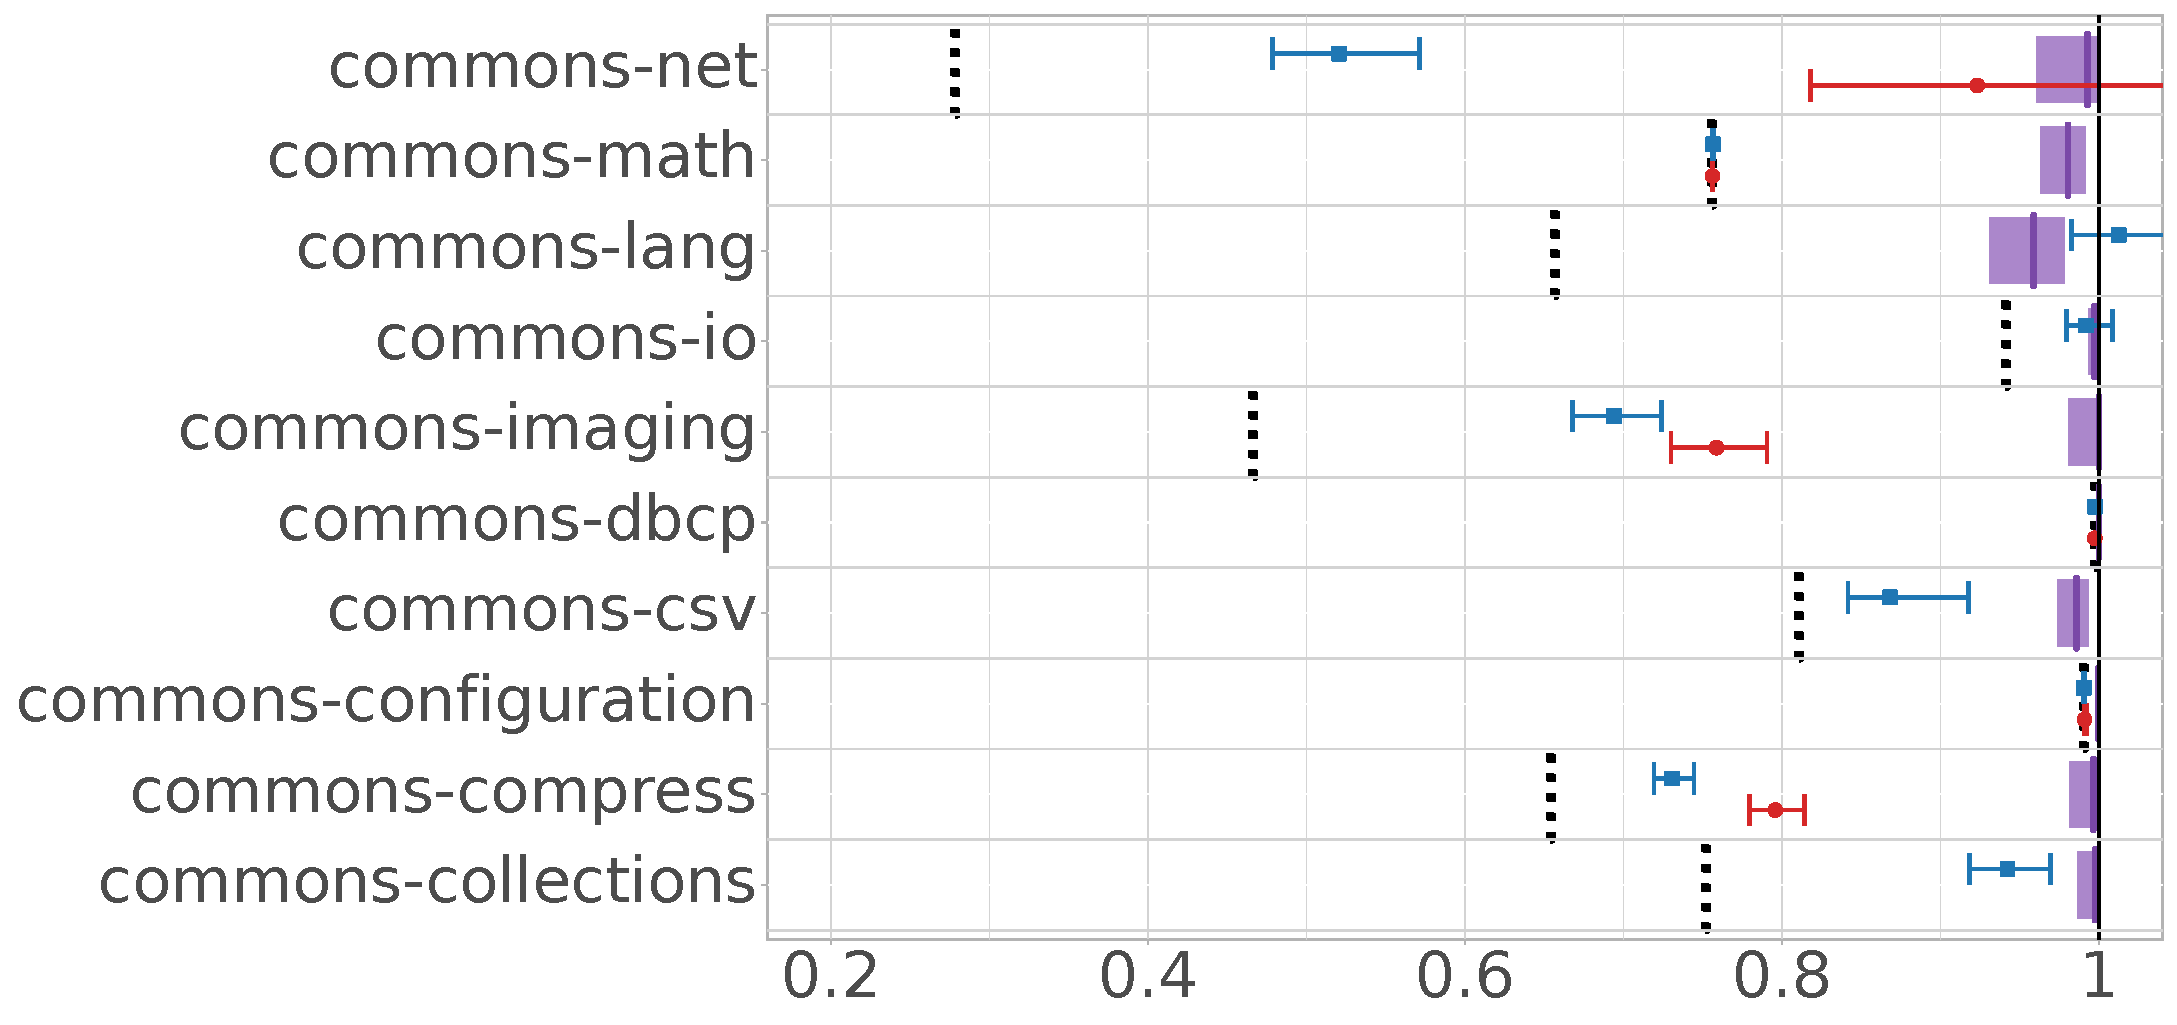
\includegraphics[width=0.98\linewidth]{chaoplots/3/Chao-organic.pdf}
%\vspace*{-3mm}
  \caption{\original} % \textcolor{cmethod}{method}, \textcolor{cclass}{class}, \textcolor{cgroundtruth}{manual}}
\label{fig:groundtruth1}
\end{subfigure}
\begin{subfigure}{.27\textwidth}
  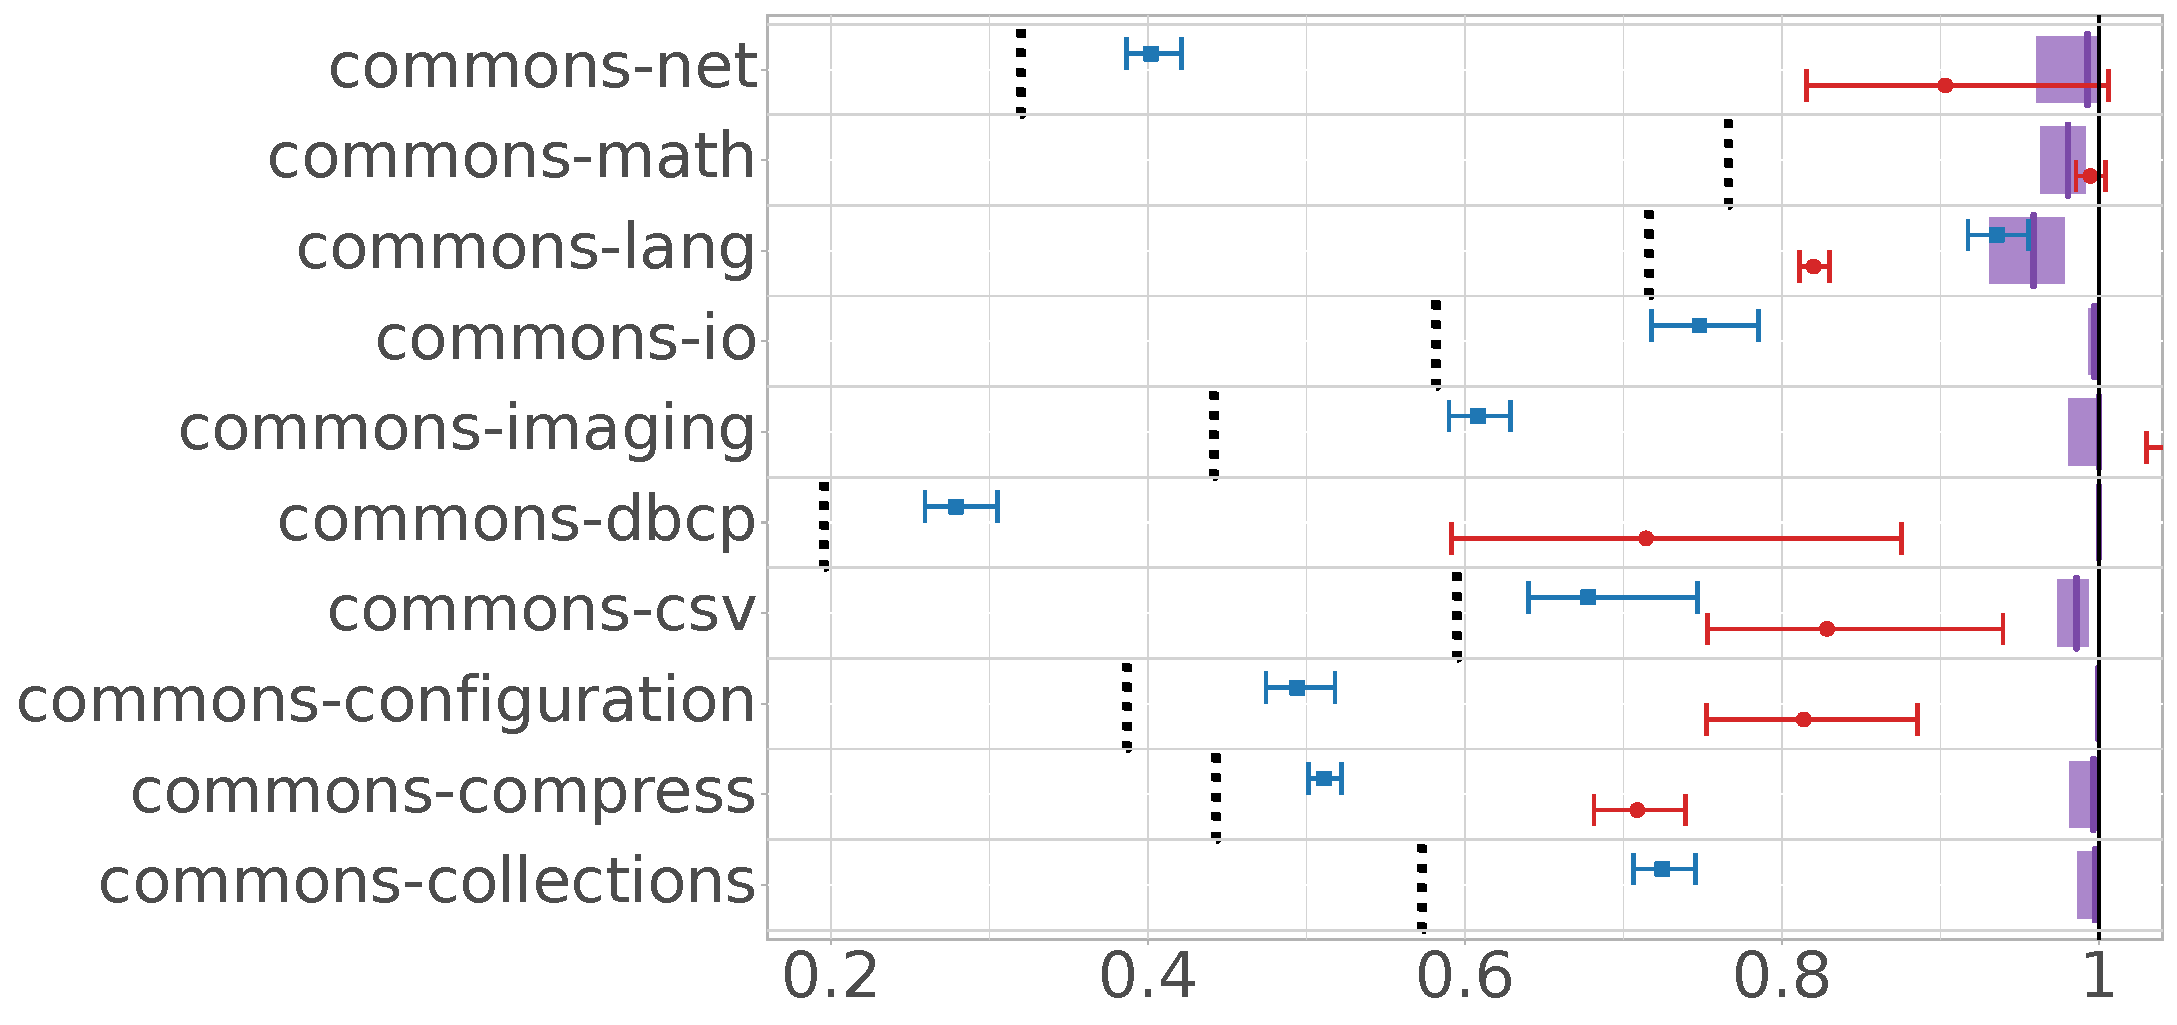
\includegraphics[width=1\linewidth,trim=12.8cm 0cm 0cm 0cm, clip=true]{chaoplots/3/Chao-random.pdf}
%\vspace*{-3mm}
\caption{\EvosuiteRandom} % \textcolor{cmethod}{method}, \textcolor{cclass}{class}, \textcolor{cgroundtruth}{manual}}
\label{fig:groundtruth3}
\end{subfigure}
\begin{subfigure}{.27\textwidth}
      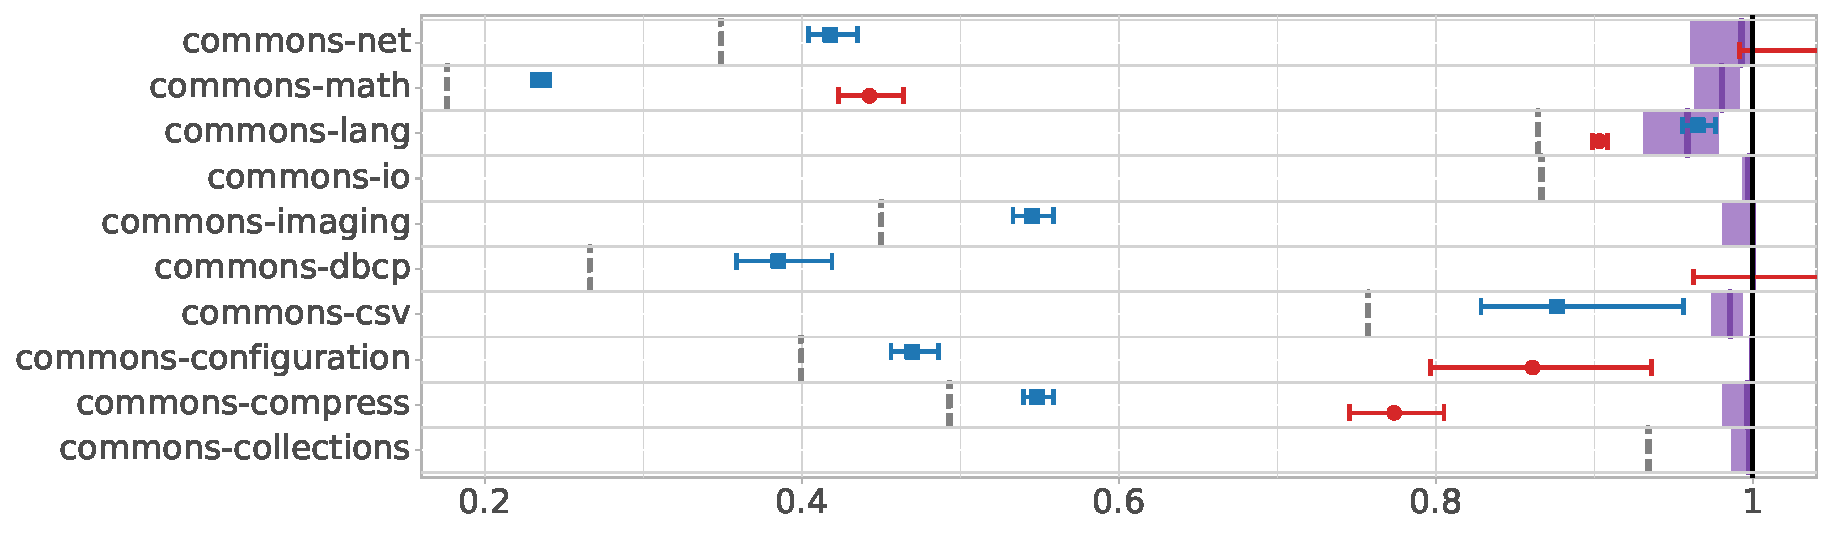
\includegraphics[width=\linewidth,trim=12.8cm 0cm 0cm 0cm, clip=true]{chaoplots/3/Chao-dynamosa.pdf}
%\vspace*{-3mm}
\caption{\EvosuiteDynamosa} % \textcolor{cmethod}{method}, \textcolor{cclass}{class}, \textcolor{cgroundtruth}{manual}}
\label{fig:groundtruth2}
\end{subfigure}
\caption{Killable mutants estimated by %frequency estimators for
 \Chao estimator and manual sampling (i.e., ground truth). %, comparison with ground truth.
Ratio of mutants in x-axis, with 1.0 indicating all generated mutants. The y-axis lists the projects.
  The method based estimators are in \textcolor{cmethod}{blue}, while class based estimators are in \textcolor{cclass}{red}.
  The \textcolor{cgroundtruth}{purple} band is the manual sampling based estimate CI, %(ground truth),
   with dark purple line the point estimate.
  The dotted black line indicates the total
  ratio of killed mutants, which is the absolute lower-bound. The figure shows how neither \textcolor{cmethod}{method} nor \textcolor{cclass}{class}
  based estimators overlap with \textcolor{cgroundtruth}{ground truth CI} consistently.}
\label{fig:groundtruth}
\end{figure*}

\begin{figure*}
\begin{subfigure}{.43\textwidth}
    \centering
      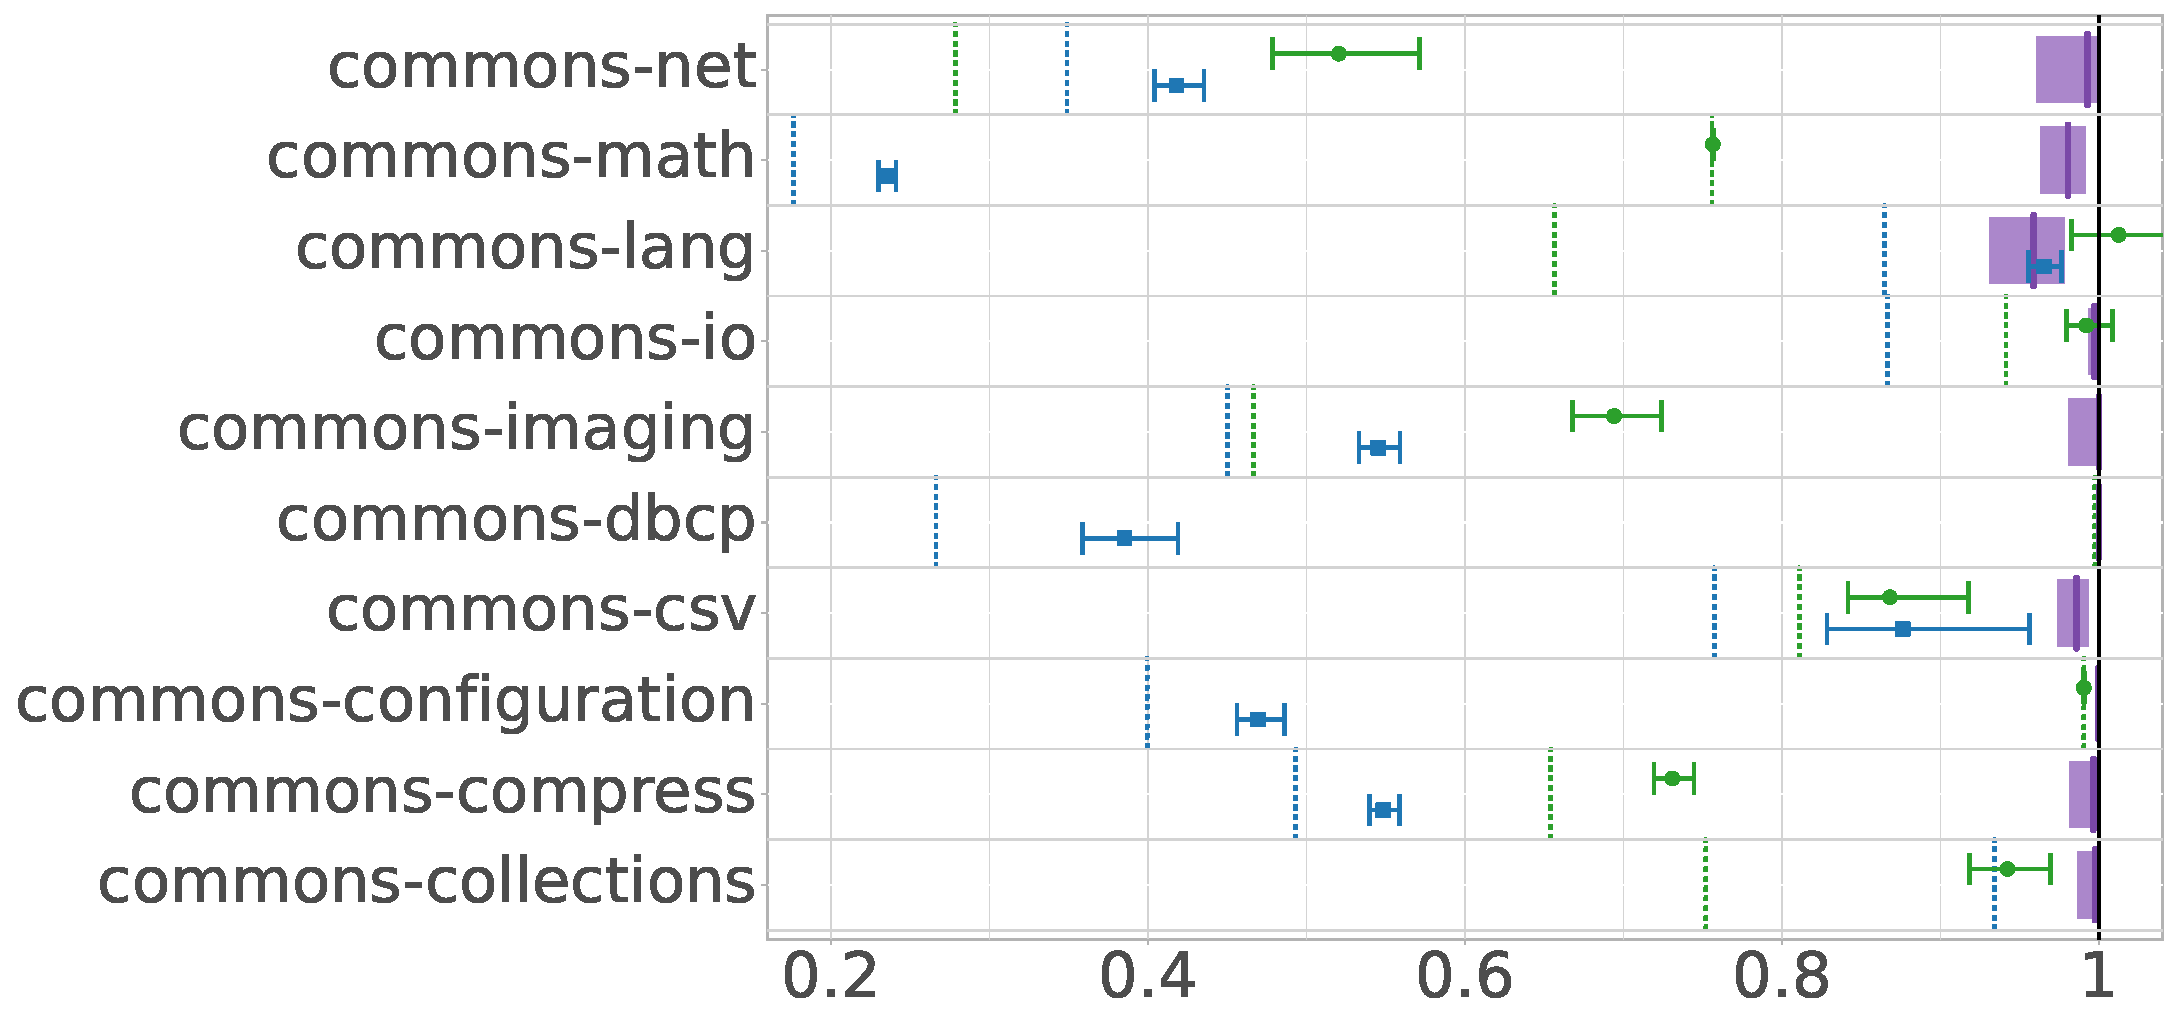
\includegraphics[width=0.95\linewidth]{chaoplots/4/Chao-methods-dynamosa-organic.pdf}
%\vspace*{-3mm}
  \caption{\textcolor{cdynamosa}\EvosuiteDynamosa vs \textcolor{coriginal}\original~(methods)}
\label{fig:am}
\end{subfigure}
\hfill
\begin{subfigure}{.28\textwidth}
    \centering
      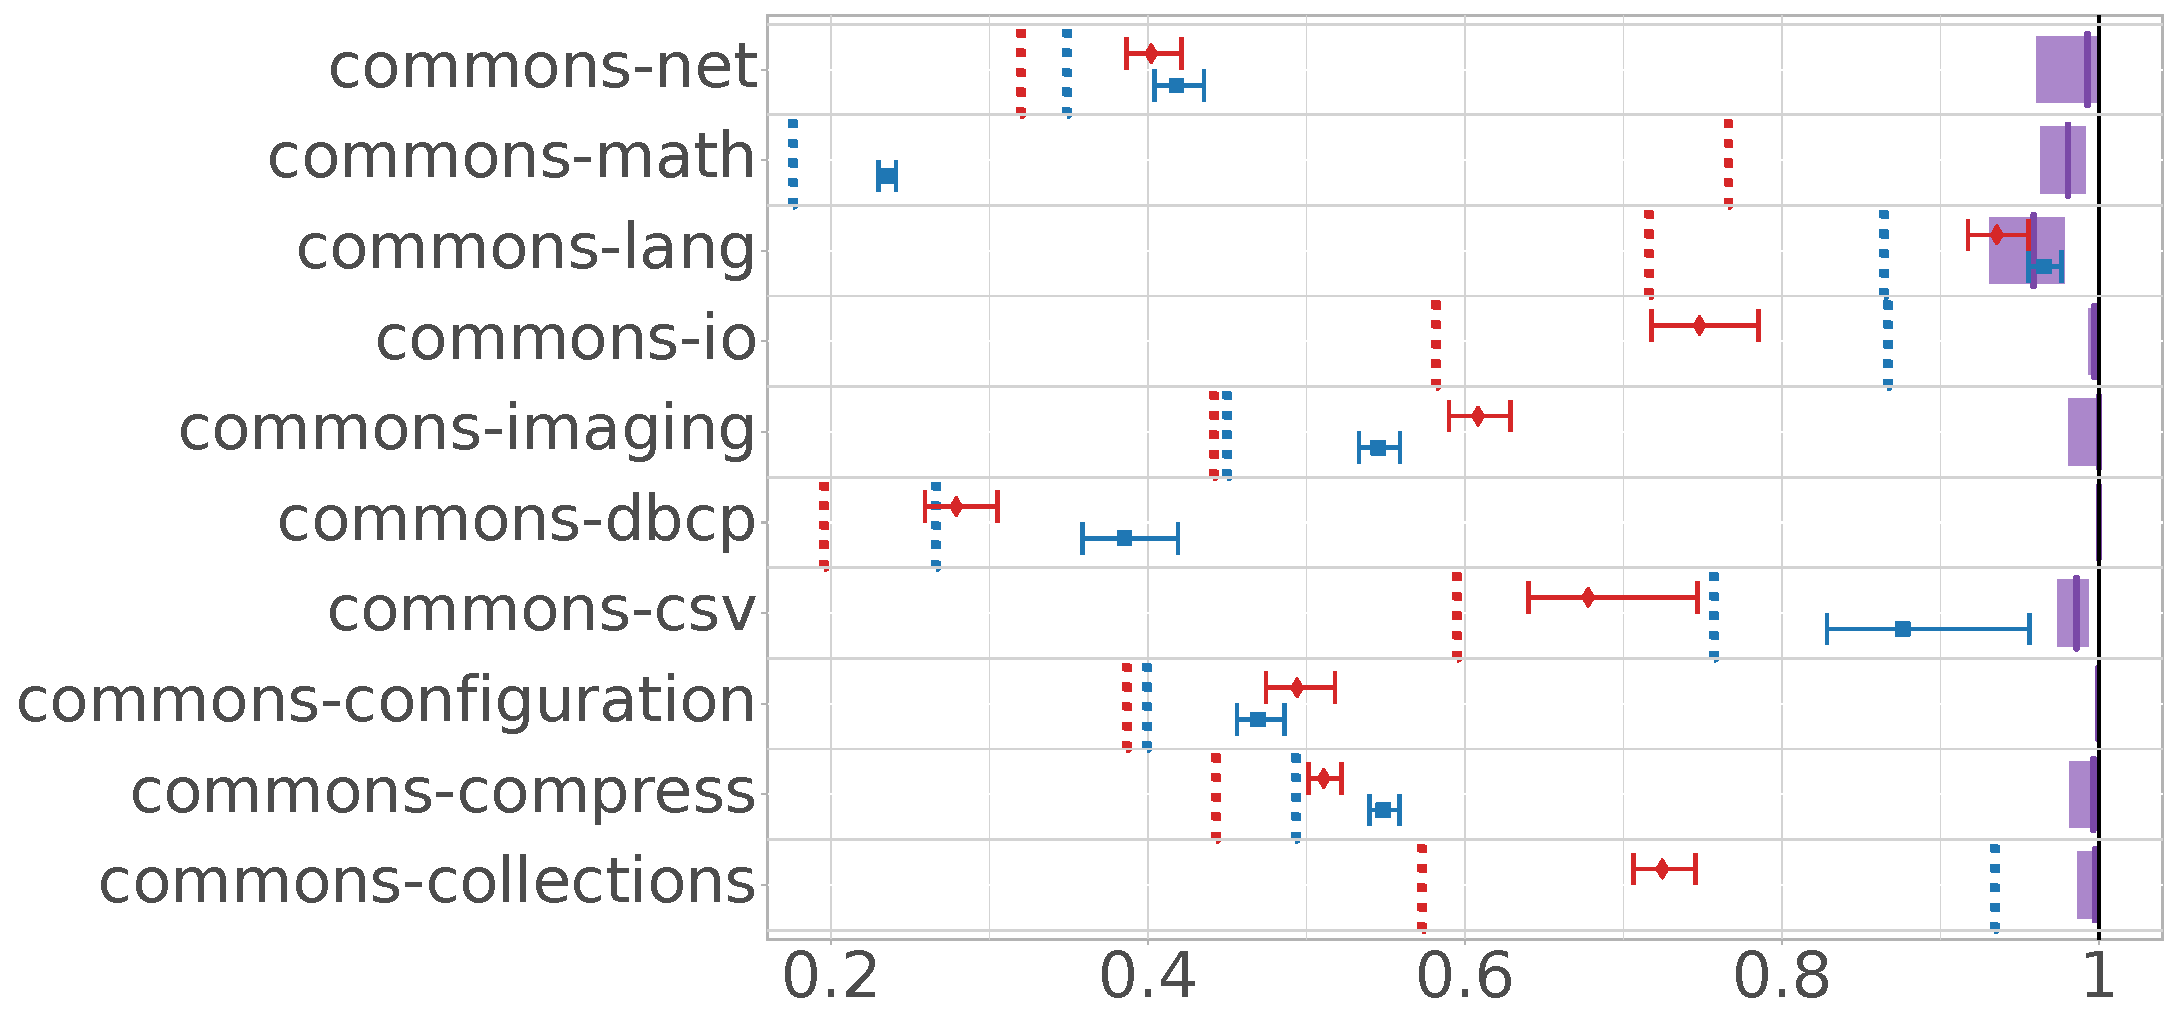
\includegraphics[width=0.95\linewidth,trim=12.8cm 0cm 0cm 0cm, clip=true]{chaoplots/4/Chao-methods-dynamosa-random.pdf}
%\vspace*{-3mm}
\caption{\textcolor{cdynamosa}\EvosuiteDynamosa vs \textcolor{crandom}\EvosuiteRandom~(methods)}
\label{fig:bm}
\end{subfigure}
\begin{subfigure}{.28\textwidth}
    \centering
      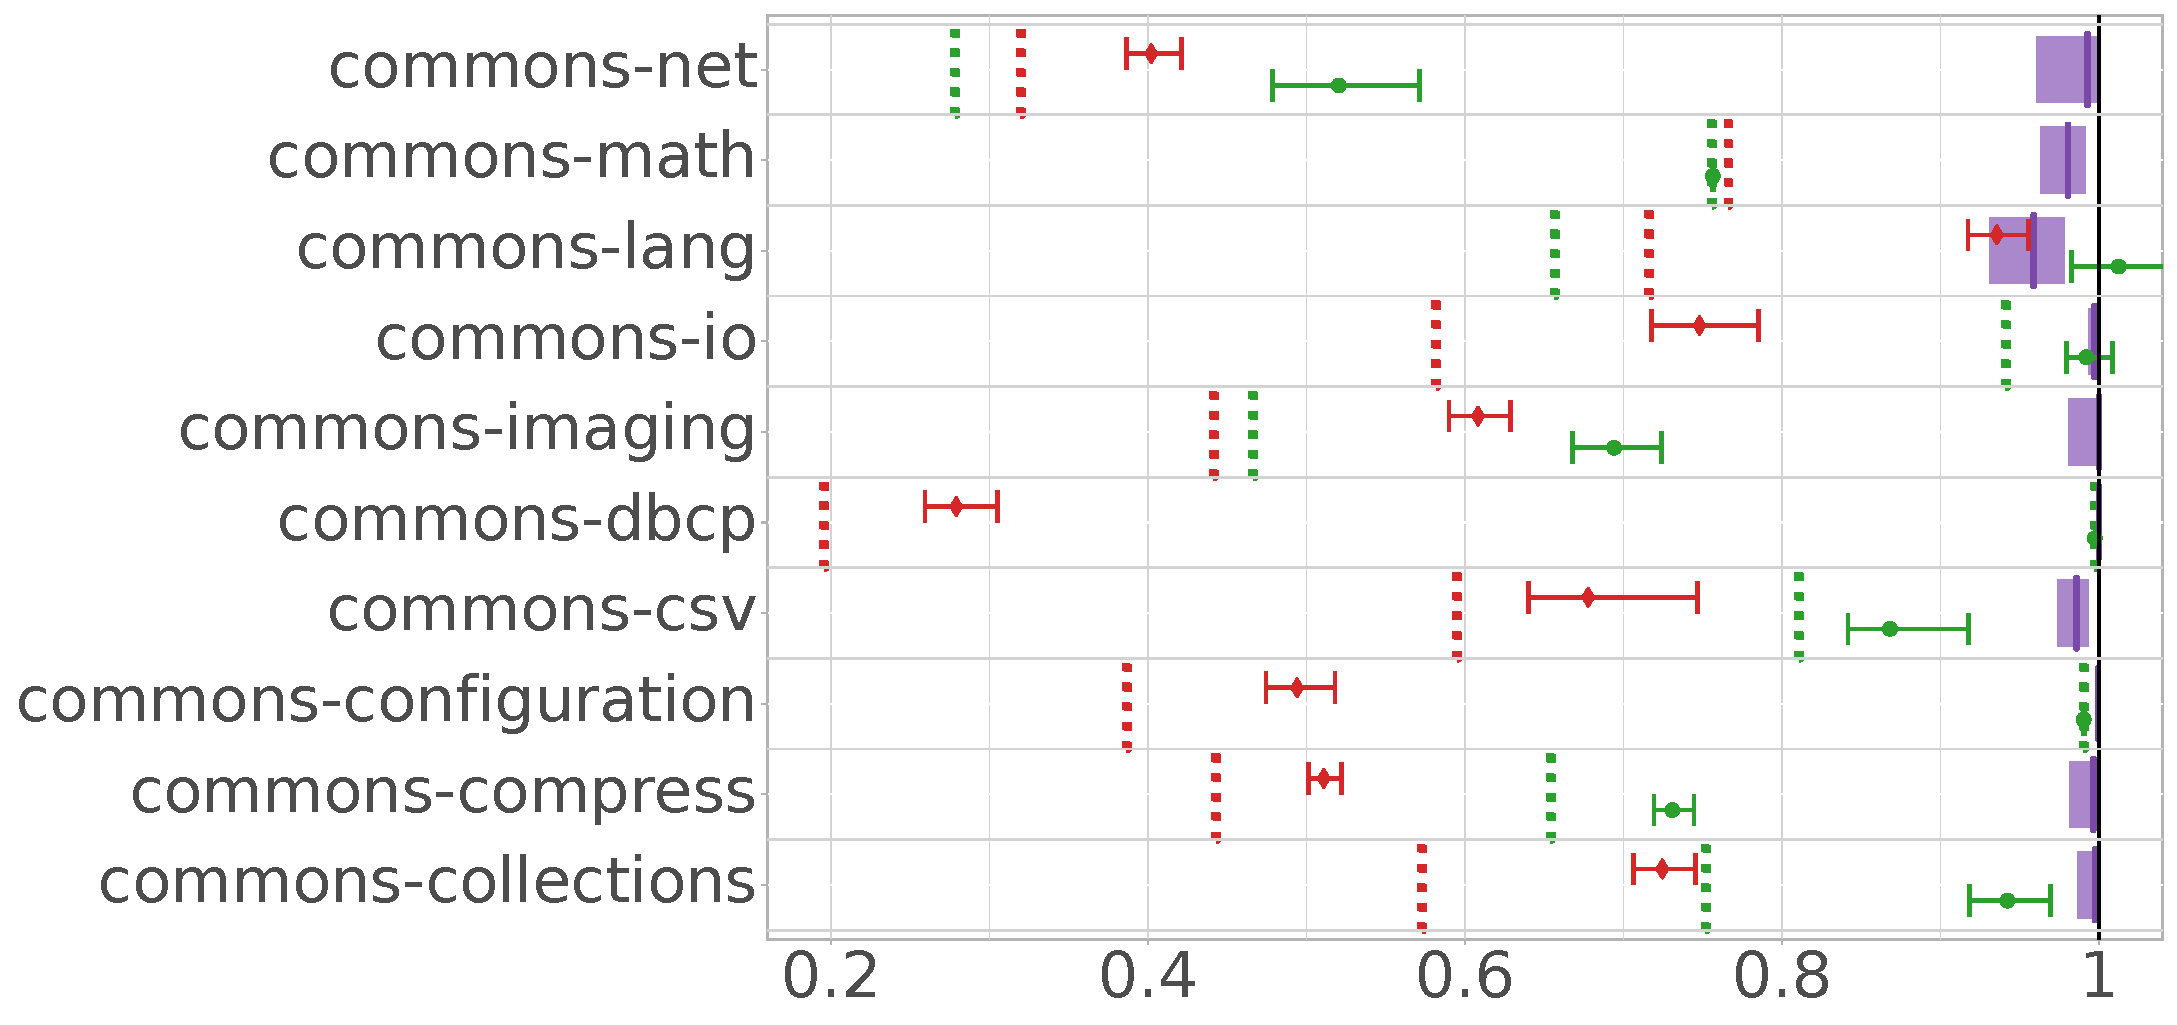
\includegraphics[width=0.95\linewidth,trim=12.8cm 0cm 0cm 0cm, clip=true]{chaoplots/4/Chao-methods-organic-random.pdf}
%\vspace*{-3mm}
\caption{\textcolor{coriginal}\original vs \textcolor{crandom}\EvosuiteRandom~(methods)}
\label{fig:cm}
\end{subfigure}
%\caption{Comparison of estimates from different test suites with \textbf{methods} as sampling unit for \Chao estimator.
%  The \original is \textcolor{coriginal}{green}, 
%  \EvosuiteDynamosa is \textcolor{cdynamosa}{blue},
%  and \EvosuiteRandom is \textcolor{crandom}{red}. The figure shows that the estimate CI from none test suites overlaps each other or ground truth consistently.}
%\label{fig:methodsamplingunit}
%\end{figure*}

%\begin{figure*}
\begin{subfigure}{.43\textwidth}
    \centering
      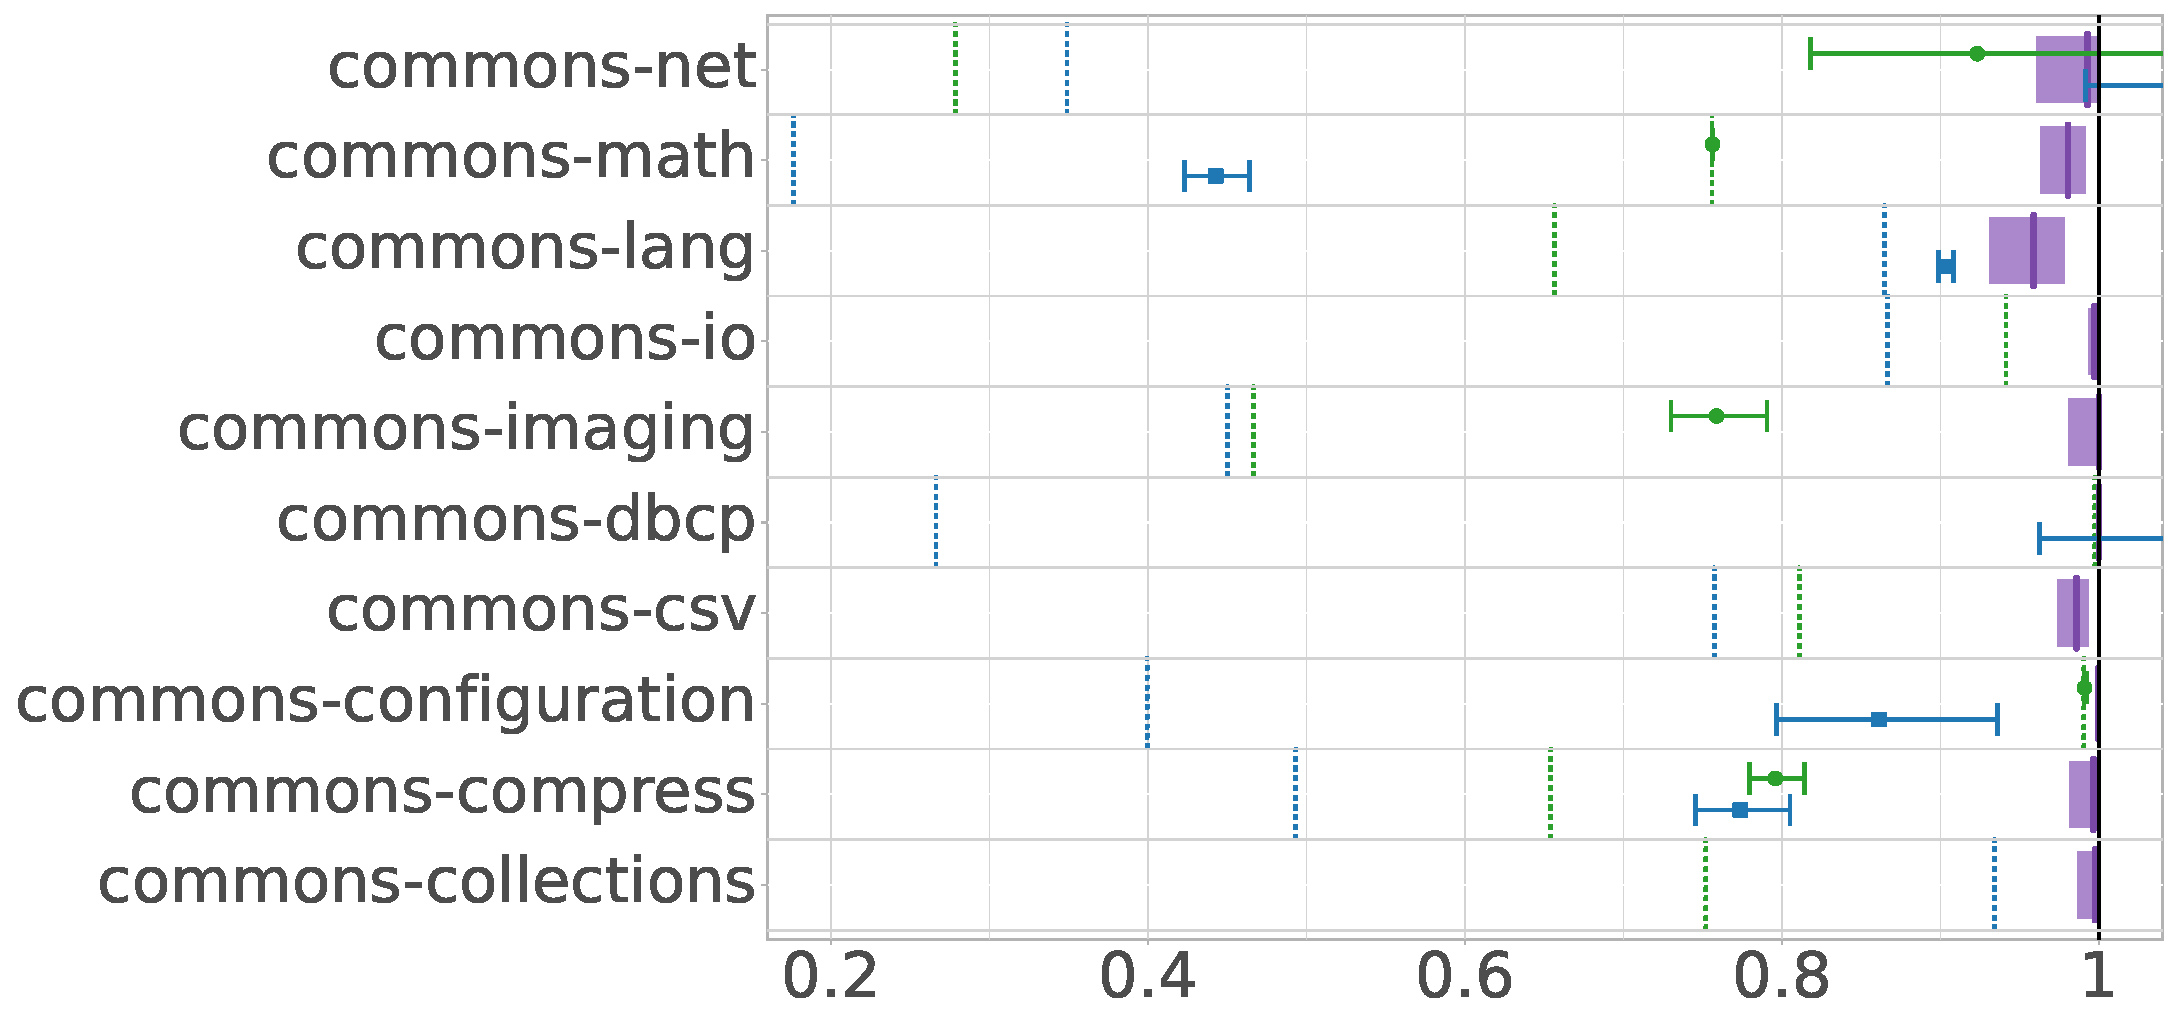
\includegraphics[width=0.95\linewidth]{chaoplots/4/Chao-classes-dynamosa-organic.pdf}
%\vspace*{-3mm}
  \caption{\textcolor{cdynamosa}\EvosuiteDynamosa vs \textcolor{coriginal}\original~(classes)}
\label{fig:ac}
\end{subfigure}
\hfill
\begin{subfigure}{.28\textwidth}
    \centering
      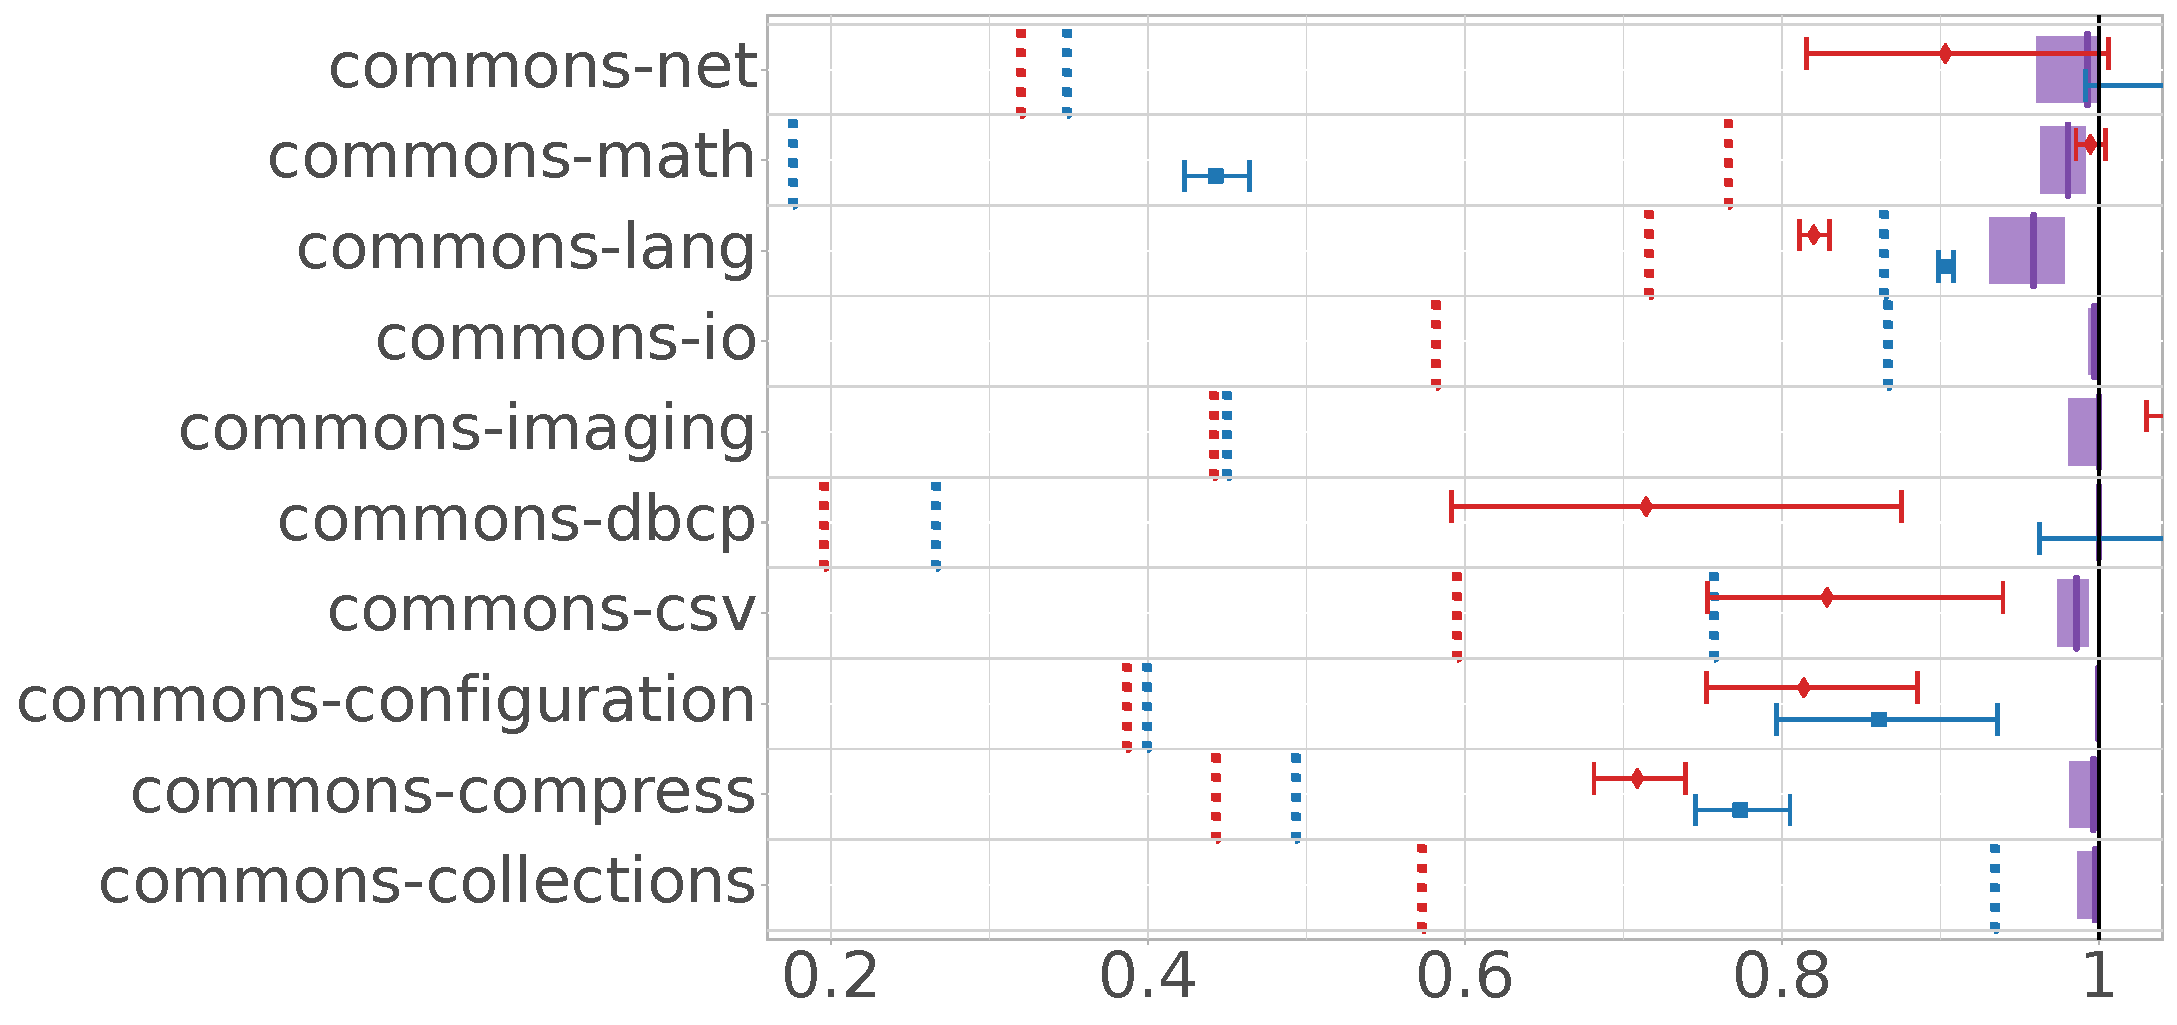
\includegraphics[width=0.95\linewidth,trim=12.8cm 0cm 0cm 0cm, clip=true]{chaoplots/4/Chao-classes-dynamosa-random.pdf}
%\vspace*{-3mm}
  \caption{\textcolor{cdynamosa}\EvosuiteDynamosa vs \textcolor{crandom}\EvosuiteRandom~(classes)}
\label{fig:bc}
\end{subfigure}
\begin{subfigure}{.28\textwidth}
    \centering
      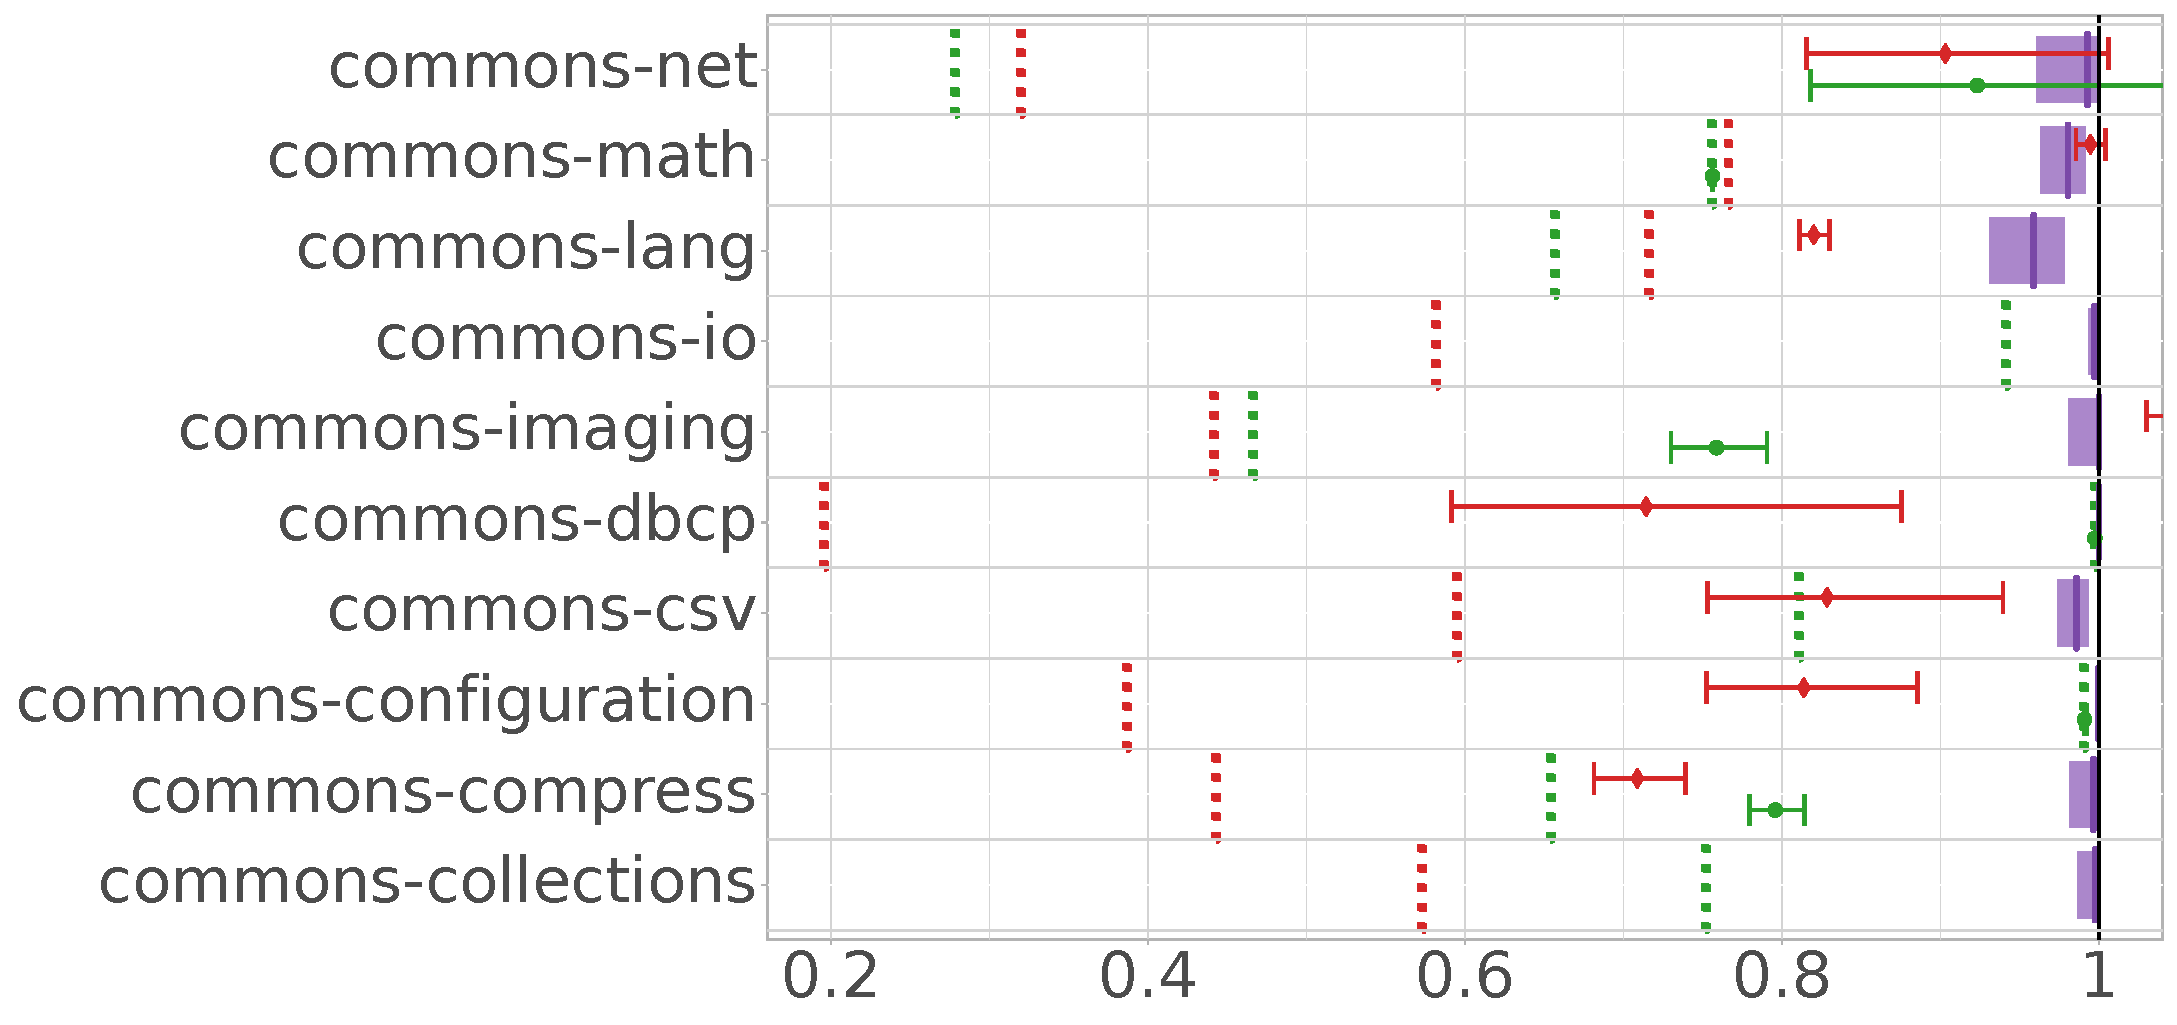
\includegraphics[width=0.95\linewidth,trim=12.8cm 0cm 0cm 0cm, clip=true]{chaoplots/4/Chao-classes-organic-random.pdf}
%\vspace*{-3mm}
  \caption{\textcolor{coriginal}\original vs \textcolor{crandom}\EvosuiteRandom~(classes)}
\label{fig:cc}
\end{subfigure}
  \caption{Comparison of estimates from different test suites with \textbf{methods} (\Cref{fig:am}\ldots\Cref{fig:cm}) and \textbf{classes} (\Cref{fig:ac}\ldots\Cref{fig:cc}) as sampling units for \Chao estimator.
  The \original is \textcolor{coriginal}{green}, 
  \EvosuiteDynamosa is \textcolor{cdynamosa}{blue},
  and \EvosuiteRandom is \textcolor{crandom}{red}. The figure shows that the estimate CI from none test suites overlaps each other or ground truth consistently.}
\label{fig:classsamplingunit}
\end{figure*}
\vspace{-4mm}

\RQBx
% As we noted in the introduction, 
%Statistical 
Frequency-based estimators rely on the data obtained by sampling campaigns;
thus, it is possible that they %frequency-based estimators
may not be robust to bias in sampling, e.g., bias introduced by the developers.
% To mitigate this bias, 
To study how different sampling strategies affect the statistical estimators,
we generated two test suites automatically, i.e., without manual bias:
\EvosuiteRandom (results in \Cref{tbl:estrandom}) and \EvosuiteDynamosa (results in \Cref{tbl:estdynamosa}).


% The results from \Cref{tbl:estrandom} for \EvosuiteRandom,
% (and \Cref{tbl:estoriginal} for \original)
% reveals that overlaps between CI from manual classification and
% \EvosuiteRandom was considerably fewer than that between manual and \original.
% The smallest difference in MD was observed for \ICEallrare,
% (mean 19.51\%, Stdev. 21.08\%). However, \ICEallrare
% had just two \emph{valid estimates}.
% For every other estimator, while the number of
% \emph{valid estimates} were considerably better, the number of CI overlaps were
% still dismal, and had a much larger mean difference, all above 30\%.

%\Cref{tbl:estrandom} reports the results obtained using \EvosuiteRandom,
%whereas \Cref{tbl:estdynamosa} the results obtained using \EvosuiteDynamosa.
%
Comparing the data in tables \ref{tbl:estoriginal}~and~\ref{tbl:estrandom}
reveals that with \EvosuiteRandom
(i) the estimators produced more valid estimates ($97$ vs. $79$);
(ii) the number of overlaps between CI from the estimators and manual classification
was comparable ($12$ vs. $13$), although not all the estimators behaved consistently;
\todo{ALESSIO: some lost, some gain, the majority stayed the same}
and, (iii) the mean difference degraded considerably ($+20\%$ on average).
% \EvosuiteRandom was considerably fewer than that between manual and \original.
% The smallest difference in MD was observed for \ICEallrare,
% (mean 19.51\%, Stdev. 21.08\%). However, \ICEallrare
% had just two \emph{valid estimates}.
% For every other estimator, while the number of
% \emph{valid estimates} were considerably better, the number of CI overlaps were
% still dismal, and had a much larger mean difference, all above 30\%.

% For \EvosuiteDynamosa, the situation was no better (\Cref{tbl:estdynamosa}),
% \ICEallrare which had the smallest mean difference (5.54) had just one valid
% estimate. Other estimators had larger MD, and few CI
% overlaps.

Comparing the data in tables \ref{tbl:estoriginal}~and~\ref{tbl:estdynamosa}
reveals that the situation did not improve using \EvosuiteDynamosa.
%an advanced test generation algorithm.
Although the valid estimates with \EvosuiteDynamosa are comparable to those with \original ($80$ vs. $79$),
the number of CI overlaps was smaller ($9$ vs. $13$) and the mean difference was even larger than \EvosuiteRandom ($+24\%$ on average).

As before, we plot the results for \Chao estimator with each sampling strategy %, the estimator suggested by the STADS framework in - ALESSIO: Repeated
in \ref{fig:groundtruth3} and ~\ref{fig:groundtruth2}.
We also plot the results for \Chao estimator test suite pairs across \Cref{fig:am}\ldots\Cref{fig:cc} along with the manual estimate.
%~\ref{fig:groundtruth3} and ~\ref{fig:groundtruth2}.
%\Cref{fig:methodsamplingunit}
%the comparison of the sampling strategies in pairs.% and \Cref{fig:classsamplingunit}
%
\todo{ALESSIO: Is this just reshuffling the content of the Figure 3? Do we really need it?}
\todo{ALESSIO: We should comment something about the figure...}
%


We expected that using automated test generation strategies would mitigate
manual bias and hence result in better estimates. Likewise, we expected that
using unbiased sampling, i.e., random search, would produce better results than
otherwise.
%
Our expectations were met %but 
only partially.


We expected that if the estimators were robust to sampling strategies used,
the estimates in each pairs would coincide. However, we found significant
differences between each pair.
Sampling killable mutants using \EvosuiteRandom, the estimators performed better
than with \EvosuiteDynamosa, confirming that unbiased sampling is beneficial. 
Moreover, the estimators produced more valid estimates with \EvosuiteRandom than any other sampling strategy.
However, we also observed that with \EvosuiteRandom the mean difference, i.e., the precision of the estimations,
drastically worsened compared to \original and that with \EvosuiteDynamosa the situation worsened.
%
% One may argue that it means that our generated test suites did not adequately
% sample the population. However, if the estimators were actually performing
% correctly, this should have resulted in a larger confidence interval, which
% would increase the \emph{accuracy} at the expense of \emph{precision}, and
% would have resulted in a larger number of overlaps.
%
One possible explanation of these results is that the automatically generated test suites
did not adequately sample the population (see statement and branch coverage in \Cref{tbl:subjectmeasures}).
However, our counterargument is that if the estimators were actually performing as expected,
they should have produced larger confidence interval, hence increasing
the \emph{accuracy} of the predictions, i.e., the number of CI overlaps,
at the expense of their \emph{precision}, i.e., mean difference.
%
But this was not the case; therefore, we answer \RQB as follows:
\begin{tcolorbox}[boxrule=0.5pt, arc=4pt, boxsep=0pt, width=\columnwidth]
The estimation quality is affected by the sampling strategy. For instance,
unbiased sampling improved the reliability of the estimators but reduced their precision.
Additionally, no matter the chosen sampling strategy, none of the estimators showed
satisfactory results.
%   The difference between estimates from \EvosuiteRandom and \EvosuiteDynamosa
% to the estimates from manual classification is statistically significant for
% every estimator examined.
\end{tcolorbox}


\RQCx
% As we mentioned in the introduction, there is a possibility, however remote,
% that the manual estimation result was either in error, or the result was a
% statistical fluke. To discount this possibility we conducted the third
% experiment, where we compared estimators based on how they predict the same
% quantity when sampling units were changed. We expected individual estimators to
% return the same predictions irrespective of the sampling units used.
\RQB showed that the estimators are affected by the sampling strategy,
i.e., the bias in sampling of killable mutants. \RQC, instead, focuses on the
granularity at which sampling happens, i.e., the sampling unit.
%
Using the same sampling strategy but different granularities, i.e., test method and class,
we expect estimators to produce comparable results, as they
predict the same quantity. Therefore, studying this aspect would let us draw
conclusions on the estimators' consistency. Moreover, this study could let us
discount the possibility that either the manual classification was incorrect
or the (bad) results achieved in \RQA were a statistical flukei---which would
be the case if the estimators from other test generators coincide.
%
% As we mentioned in the introduction, there is a possibility, however remote,
% that the manual estimation result was either in error, or the result was a
% statistical fluke. To discount this possibility we conducted the third
% experiment, where we compared estimators based on how they predict the same
% quantity when sampling units were changed. We expected individual estimators to
% return the same predictions irrespective of the sampling units used.


From \Cref{tbl:estoriginalclassmethod}, \Cref{tbl:estrandomclassmethod},
and \Cref{tbl:estdynamosaclassmethod}, we observe that the 
estimates from method and class level sampling units
are %statistically
significantly different.
Even \Bootstrap, which had the highest (50\%) overlap for \EvosuiteRandom, 
did not produce a significant overlap of CI between method and class estimators
for other test suites.

This situation is clearly exemplified in \Cref{fig:groundtruth}
%figures \ref{fig:groundtruth1}, \ref{fig:groundtruth3}, and \ref{fig:groundtruth2}
for \Chao estimator, in which almost all the CIs for the same test subject
and sampling strategy do not overlap.

In light of these results, we answer \RQC:
\begin{tcolorbox}[boxrule=0.5pt, arc=4pt, boxsep=0pt, width=\columnwidth]
The difference between estimates from test method and test class level
estimators %to the estimates from manual classification
is statistically significant for every estimator examined. Consequently,
none of the \estimatorCount estimators was robust against changes in sampling
unit.
\end{tcolorbox}
\subsection{Additional Observations}
From a detailed analysis of the data (see Appendix~\cite{replication-package} for detailed plots and tables)
we also observe that (1) method estimators for different test suites for same
subjects overlap and have a smaller variance than class estimators, and (2) method
estimators often (but not always) appear to underestimate compared to
the manual estimates, while the same cannot be said for class estimators.
(3) Bootstrap tends to produce consistent estimates for method and class
estimators with small CIs when the number of mutants killed is far from the total
generated. However, the uncertainties in CI increase drastically as the
number of killed mutants approaches the total generated. We observe the opposite
behavior in all other estimators. (4) In a significant number
of subjects, the difference between class and method estimators seems to
diminish as the number of killed mutants approaches the total generated.
This is an intriguing hint because the total number of generated mutants is
not part of the estimator equations. Hence, it is likely that the observed
pattern is linked to the total of killable mutants, which is close to the total of
generated mutants.
(5) Finally, we observe that the plots vary
considerably based on the subject in question.
While there are several other interesting patterns in the data, the data we have
is insufficient to explore these fully. Therefore, we will refrain
from interpreting these until a larger follow-up study can be
conducted.

\subsection{What Does This Mean in Practice?}
For an estimator to be useful to the developers, it should be able to produce
estimates that are accurate and precise. Additionally, the estimators must be reliable, i.e.,
its ability to produce valid estimates should not strongly depend on the project under analysis.

We note that examination of just $100$ mutants is sufficient to produce an
estimate within $2\%$ of the true value. Assuming that examining $100$ mutants is
reasonable, we should expect any equivalent mutant estimator to do better than
this value. However, the fact that none of the estimators could consistently
produce estimates that are close to the manual estimates suggests that the
frequency-based estimators are not yet ready for use by developers.

To verify that our manual analysis was not the cause of an error, we also
investigated whether the estimators could produce consistent values when
estimating the same quantities but using different sampling units---method and class.
We observed that the estimates produced were inconsistent, i.e., only few CIs overlapped.
%s of the CI. 
This is a cause for concern and points to violated assumptions in the
underlying model, which needs to be investigated further.

While overall, the result of our study is negative, we observe a glimmer of hope.
We note that in \Cref{tbl:estrandomclassmethod} comparing method and class sampling
units using \EvosuiteRandom, \Bootstrap produced $50\%$ CI overlaps. Furthermore,
the mean difference was $6.79\%$ with a similarly small standard deviation
of $2.71\%$. It is possible that not all the mutants that can be killed manually
may be killable by automatic test generators due to technical limitations or
deficiencies in the test oracles. Hence, it is possible that \Bootstrap estimation is true to the
actual value, albeit with a large amount of uncertainty.

Furthermore, unlike \EvosuiteDynamosa, \EvosuiteRandom is unguided in
test generation, which may be a hint as to the better performance of \Bootstrap
on \EvosuiteRandom and points to the need for further study.


%\done{
%ALESSIO: We mention already Cohen's Kappa for the classification}
%RAHUL: The following two sections are necessary by ESEM requirements.
%
\noindent\textbf{Empirical Strategy Used.}
This paper uses the quantitative research, including systematic
collection of data about different mutants and comparing classifications by
different experts, and the agreement is computed by Cohen's Kappa.%\todo{TODO}

\noindent\textbf{Data Availability.}
The replication package~\cite{replication-package} contains data about manual
classification of mutants, test suites, kill matrices, and scripts
to compute and plot estimations.
The data will be made publicly available.

\section{Threats to Validity}
\label{sec:threats}

\noindent\textbf{External Validity.}
Our study was conducted on a limited number of programs from a specific
open-source repository and using a small number of test producers;
hence, our findings
may not generalize to other projects and test suites produced by other means.
 %other strategies (e.g., model-based, single object genetic algorithm)
To reduce this risk, we selected multiple projects from Apache Commons and
used EvoSuite in two exemplary configurations.
Apache Commons projects are popular, implement different functionalities, and
are comparable to % generally compared to seen to have similar quality as in 
well run industrial projects.
EvoSuite, instead, implements standard baselines %(e.g., random) 
and
well established and effective algorithms %(e.g., DynaMOSA), 
that generate test suites with remarkably different features.
We use a single run of both the test generator (randomized) on our classes.
While multiple runs are required for statistical confidence of the results,
we note that our approach is similar to the one adopted by established biometrics
studies that draw conclusions from single sampling campaigns.

\noindent\textbf{Internal Validity.}
Automatically generated test suites did not always achieve high coverage;
hence, they can lead to larger uncertainty in the final estimation of equivalent mutants. 
However, we note that this situation is similar to the one currently faced by software practitioner. % has to contend with.
Next, our analysis can be subject to bugs, sampling errors, and manual-misclassification of mutants 
as equivalents.
%that might bias our results.
%For instance, the test generator could not generate unit tests for all the classes under analysis,
%thus failing to sample their mutants.
We tried to mitigate this risk by reviewing the code of JUGE and our scripts, 
cross-checking the results, and use the largest possible subset of classes for which
test generation succeeded.
It is possible that our manual classification is biased. We tried to mitigate it by cross-checking between three classifiers.

\noindent\textbf{Construct Validity.} We are the first to apply
frequency-based statistical models %species richness 
to the problem of killable mutants estimation; hence, 
our mapping of statistical estimators to the mutation testing domain
might not to capture important variables. %We also acknowledge this threat.
We tried to mitigate this threat by adopting different sampling strategies.

\section{Related Work}
\label{sec:related}
Mutation analysis is considered a primary way of evaluating test quality~\cite{papadakis2019mutation};
thus, mutation score is usually considered as a test suite adequacy metrics~\cite{just2014are,andrews2005is,andrews2006using,daran1996software}. 
Unfortunately, equivalent mutants have vexed practitioners from the very beginning~\cite{budd1982two}
and remain an open issue~\cite{madeyski2014overcoming} that affects also residual risk estimation.
To address this issue, we proposed to estimate killable mutants using
frequency-based statistical estimators that have been applied recently to
estimate reachable coverage
and conducted a large empirical study that included
$10$ mature open-source Java projects, $3$ types of test suites, and the 
manual classification of $1016$ live mutants involving $3$ researchers.

\noindent\textbf{Studies focusing on estimating killable or equivalent mutants.}
Papadakis et al.~\cite{papadakis2014mitigating} conducted a study
for estimating killable mutants with more numerous subjects.
We note that this approach requires manual classification,
however limited, for residual defect estimation.
This may not be feasible in many cases where the testers may not be program experts.
Furthermore, evaluating residual risk may be conducted by
people who are not involved in either testing or development (such as the end-user).
Hence, alternative means of estimating killable mutants is required.

In comparison to the mutant classification performed in Papadakis et al.~\cite{papadakis2014mitigating},
our study considers larger programs and different test suites, do not employ selective
mutation, whose limits have been discussed empirically and
theoretically~\cite{gopinath2017mutation,gopinath2016on}, and we employ
mechanisms such as conflict identification and resolution, to reduce manual
classification error proneness.

Vincenzi et al.~\cite{vincenzi2002bayesian} proposed
estimating the (posterior) probability that specific mutation operators
generate equivalent mutants.
Marsit et al.~\cite{marsit2017estimating,marsit2018impact,ayad2019estimating}
proposed using information theory %(e.g., entropy) 
to measure the intrinsic \emph{redundancy} in programs as a proxy for mutants equivalence. 
Despite their potential benefits and promising initial results,
none of those methods has been empirically evaluated yet.

\noindent\textbf{Studies conducting mutant classification.}
A few previous studies also relied on the manual mutants classification.
Acree's study~\cite{acree1980mutation} 
involved two competent software engineers experts in mutation analysis
that classified
live mutants from four COBOL programs.
Similar to our classification procedure, Acree used manually written tests
for eliminating a large chuck of mutants; however, differently 
from us, the classifiers had no exposure to the programs under analysis and
focused on small COBOL programs.
During his study, Acree documented various misclassifications (avg. 23\%),
suggesting that even manual classification has errors. 
We also found misclassifications (see \Cref{tbl:classified}, \emph{Misclass.} column),
but achieved better accuracy~(less than $5\%$ misclassifications on avg),\footnote{This measure does not consider the results of \texttt{commons-csv} that we used for training the labelers.}
arguably because we trained the labelers
and followed a structured and systematic classification protocol.

Other studies of note are by Yao et al.~\cite{yao2014a} on $18$ C programs,
and Gr\"un et al.~\cite{grun2009impact} (extended by Schuler et al.~\cite{schuler2010covering})
on $7$ Java programs.
Both studies involved a single researcher but classified a different amount of live mutants,
$1,194$  Yao et al. and %drastically few (i.e., $140$) Gr\"un et al.
$140$ Gr\"un et al.
Yao et al.'s study 
estimated that 77\% of all mutants are killable, while Gr\"un et al.'s reported that 
45\% of the \emph{classified} live mutants are equivalent.
Unfortunately, none of those studies reported the misclassification rate.
Compared to those studies, 
our manual classification required (modulo the number of mutants) the same amount of time, 
but involved twice as many researchers. We also considered real-world, more complex, and arguably more
difficult to evaluate, projects, and a representative set of mutation operators~\cite{gopinath2017mutation}.
Finally, we studied manually written and automatically generated unit test suites, 
that covered more mutants and estimating a higher number (generally $> 90$\%) of killable mutants.

We used statistical estimators for predicting killable mutants, others, instead, used
them for estimating residual faults.
For instance, B{\"o}hme~\cite{bohme2018stads} argued to use the same
species richness estimators we studied for estimating residual defect density,
while Nayak~\cite{nayak1988estimating} and Voas~and~McGraw~\cite{voas1997software}
modeled faults and 
residual defects as members of unknown populations
and estimated their number via \emph{capture-recapture} methods.
Tohma et al.~\cite{tohma1989structural}, instead, modeled
the distribution of observed faults as hyper-geometric distribution
to estimate the number of residual defects.

\section{Conclusions and Future Work}
\label{sec:conclusions}
Accurately estimating the number of killable mutants is crucial for estimating
the residual risk and the effectiveness of test generators.
While a sound and complete classifier for killable and equivalent mutants is impossible,
recent advances in statistical estimation using frequency %count 
based estimators gave us hope that one could at least estimate the number of killable mutants.
%
Consequently, we organized the first, large evaluation of these estimators on mutation analysis spanning several projects and multiple sampling strategies.
%
%
%This research provides the first, large evaluation of these estimators on mutation analysis. 

Unfortunately, the results we achieved show that the considered statistical estimators %for species richness 
applied to the killable mutants estimation are not ready for prime time, as they did not produce consistent, accurate, or precise estimates.
% results across projects, test suites, and when computed using different sampling strategies.
%Hence, they are, as yet, unsuitable for use as statistical estimators for
%killable mutants in mutation analysis.

Nonetheless, our observations pointed out that it 
%We also found tantalizing evidence that may indicate that
% statistical estimation
may be possible, with more sophisticated models and more data, to successfully put statistical estimation in use. 
However, further study is required to investigate this aspect.

%\bibliographystyle{ACM-Reference-Format}
\bibliographystyle{unsrt}
\bibliography{esem2024-chaos}
%
% \appendix

% \begin{table}[h]
\caption{Comparison of \emph{mean difference (MD)} between method estimators across subjects---\original test suites}
\begin{tabular}{|l|r|r|r|r|r|}
\hline
Estimator & Valid Estimates & CI Overlaps & Mean & Stdev \\
\hline
\ICEallrare & 4 & 0 & 5.78 & 6.52 \\
\Zelterman & 6 & 1 & 13.48 & 14.06 \\
\ChaoBunge & 6 & 1 & 9.77 & 11.03 \\
\Jackknife & 6 & 0 & 15.03 & 9.21 \\
\Chao & 8 & 1 & 18.19 & 16.47 \\
\improvedChao & 7 & 1 & 18.59 & 15.05 \\
\ICE & 8 & 1 & 19.22 & 16.7 \\
\improvedICE & 8 & 2 & 15.16 & 12.67 \\
\Unpmle & 6 & 2 & 13.28 & 11.0 \\
\Bootstrap & 9 & 0 & 19.76 & 20.51 \\
\Pnpmle & 5 & 1 & 17.31 & 11.84 \\
\PCG & 6 & 3 & 9.14 & 10.52 \\
\hline
\end{tabular}
\label{tbl:estoriginal}
\end{table}

\begin{table}[h]
\caption{Comparison of \emph{mean difference (MD)} between class estimators across subjects---\original test suites}
\begin{tabular}{|l|r|r|r|r|r|}
\hline
Estimator & Valid Estimates & CI Overlaps & Mean & Stdev \\
\hline
\ICEallrare & 4 & 1 & 6.26 & 9.77 \\
\Zelterman & 5 & 1 & 9.33 & 9.26 \\
\ChaoBunge & 4 & 0 & 9.64 & 10.86 \\
\Jackknife & 4 & 0 & 7.75 & 9.96 \\
\Chao & 5 & 1 & 14.89 & 10.35 \\
\improvedChao & 4 & 0 & 14.2 & 9.28 \\
\ICE & 4 & 0 & 16.54 & 10.51 \\
\improvedICE & 4 & 0 & 12.21 & 9.45 \\
\Unpmle & 3 & 0 & 11.14 & 9.63 \\
\Bootstrap & 5 & 2 & 25.83 & 22.67 \\
\PCG & 2 & 0 & 9.94 & 13.3 \\
\hline
\end{tabular}
\label{tbl:estoriginalclass}
\end{table}

\begin{table}[h]
\caption{Comparison of \emph{mean difference (MD)} between method estimators across subjects---\EvosuiteRandom test suites}
\begin{tabular}{|l|r|r|r|r|r|}
\hline
Estimator & Valid Estimates & CI Overlaps & Mean & Stdev \\
\hline
\ICEallrare & 2 & 1 & 19.51 & 21.08 \\
\Zelterman & 8 & 1 & 36.33 & 19.32 \\
\ChaoBunge & 8 & 1 & 30.95 & 17.16 \\
\Jackknife & 8 & 0 & 34.28 & 19.55 \\
\Chao & 9 & 1 & 39.42 & 20.82 \\
\improvedChao & 9 & 0 & 37.42 & 20.63 \\
\ICE & 9 & 1 & 37.79 & 20.41 \\
\improvedICE & 8 & 0 & 38.12 & 17.22 \\
\Unpmle & 8 & 2 & 39.9 & 17.42 \\
\Bootstrap & 10 & 2 & 36.53 & 23.15 \\
\Pnpmle & 9 & 1 & 35.45 & 20.76 \\
\PCG & 9 & 2 & 35.17 & 22.03 \\
\hline
\end{tabular}
\label{tbl:estrandom}
\end{table}

\begin{table}[h]
\caption{Comparison of \emph{mean difference (MD)} between class estimators across subjects---\EvosuiteRandom test suites}
\begin{tabular}{|l|r|r|r|r|r|}
\hline
Estimator & Valid Estimates & CI Overlaps & Mean & Stdev \\
\hline
\ICEallrare & 3 & 0 & 16.4 & 14.54 \\
\Zelterman & 7 & 4 & 10.65 & 9.61 \\
\ChaoBunge & 2 & 1 & 5.44 & 5.24 \\
\Jackknife & 4 & 2 & 7.23 & 6.24 \\
\Chao & 7 & 2 & 16.56 & 9.94 \\
\improvedChao & 5 & 1 & 15.56 & 5.6 \\
\ICE & 5 & 0 & 19.05 & 11.91 \\
\improvedICE & 3 & 2 & 6.5 & 0.63 \\
\Unpmle & 3 & 2 & 9.02 & 14.04 \\
\Bootstrap & 9 & 1 & 33.76 & 22.22 \\
\Pnpmle & 1 & 1 & 1.43 &  \\
\PCG & 2 & 2 & 1.56 & 1.58 \\
\hline
\end{tabular}
\label{tbl:estrandomclass}
\end{table}

\begin{table}[h]
\caption{Comparison of \emph{mean difference (MD)} between method estimators across subjects---\EvosuiteDynamosa test suites}
\begin{tabular}{|l|r|r|r|r|r|}
\hline
Estimator & Valid Estimates & CI Overlaps & Mean & Stdev \\
\hline
\ICEallrare & 1 & 1 & 5.54 &  \\
\Zelterman & 6 & 0 & 49.86 & 12.08 \\
\ChaoBunge & 8 & 1 & 39.83 & 23.29 \\
\Jackknife & 7 & 1 & 36.58 & 22.31 \\
\Chao & 8 & 1 & 43.54 & 25.27 \\
\improvedChao & 8 & 0 & 42.15 & 24.45 \\
\ICE & 8 & 1 & 43.67 & 25.09 \\
\improvedICE & 8 & 1 & 41.92 & 24.36 \\
\Unpmle & 6 & 2 & 39.16 & 29.03 \\
\Bootstrap & 7 & 0 & 49.66 & 20.85 \\
\Pnpmle & 7 & 1 & 37.72 & 19.16 \\
\PCG & 6 & 0 & 32.21 & 26.21 \\
\hline
\end{tabular}
\label{tbl:estdynamosa}
\end{table}

\begin{table}[h]
\caption{Comparison of \emph{mean difference (MD)} between class estimators across subjects---\EvosuiteDynamosa test suites}
\begin{tabular}{|l|r|r|r|r|r|}
\hline
Estimator & Valid Estimates & CI Overlaps & Mean & Stdev \\
\hline
\ICEallrare & 1 & 1 & 0.73 &  \\
\Zelterman & 3 & 0 & 24.96 & 21.6 \\
\ChaoBunge & 2 & 1 & 4.19 & 0.3 \\
\Jackknife & 1 & 0 & 37.27 &  \\
\Chao & 4 & 0 & 23.86 & 21.07 \\
\improvedChao & 4 & 0 & 19.15 & 20.24 \\
\ICE & 4 & 1 & 21.01 & 21.93 \\
\improvedICE & 3 & 1 & 15.47 & 14.95 \\
\Bootstrap & 6 & 0 & 49.04 & 15.57 \\
\Pnpmle & 1 & 0 & 1.49 &  \\
\hline
\end{tabular}
\label{tbl:estdynamosaclass}
\end{table}


% \begin{table}[h]
\caption{Comparison of \emph{mean difference (MD)} between method estimators across subjects---\original test suites}
\begin{tabular}{|l|r|r|r|r|r|}
\hline
Estimator & Valid Estimates & CI Overlaps & Mean & Stdev \\
\hline
\ICEallrare & 8 & 0 & 19.04 & 20.48 \\
\Zelterman & 9 & 1 & 15.15 & 12.27 \\
\ChaoBunge & 9 & 3 & 21.52 & 41.98 \\
\Jackknife & 9 & 0 & 15.08 & 10.24 \\
\Chao & 9 & 1 & 16.76 & 15.98 \\
\improvedChao & 9 & 2 & 15.86 & 14.39 \\
\ICE & 9 & 1 & 17.96 & 16.07 \\
\improvedICE & 9 & 2 & 16.58 & 12.59 \\
\Unpmle & 10 & 5 & 10.97 & 9.72 \\
\Bootstrap & 10 & 0 & 18.33 & 19.85 \\
\Pnpmle & 9 & 1 & 17.58 & 16.12 \\
\PCG & 7 & 4 & 7.95 & 10.1 \\
\hline
\end{tabular}
\label{tbl:estoriginal}
\end{table}

\begin{table}[h]
\caption{Comparison of \emph{mean difference (MD)} between class estimators across subjects---\original test suites}
\begin{tabular}{|l|r|r|r|r|r|}
\hline
Estimator & Valid Estimates & CI Overlaps & Mean & Stdev \\
\hline
\ICEallrare & 9 & 1 & 35.01 & 51.25 \\
\Zelterman & 9 & 1 & 35.73 & 49.73 \\
\ChaoBunge & 7 & 0 & 22.63 & 18.94 \\
\Jackknife & 10 & 0 & 40.27 & 51.54 \\
\Chao & 9 & 1 & 31.65 & 40.68 \\
\improvedChao & 9 & 1 & 34.98 & 47.4 \\
\ICE & 9 & 0 & 40.15 & 55.34 \\
\improvedICE & 8 & 0 & 39.88 & 43.26 \\
\Unpmle & 6 & 0 & 31.53 & 31.36 \\
\Bootstrap & 10 & 6 & 16.78 & 19.14 \\
\Pnpmle & 8 & 1 & 64.47 & 34.78 \\
\PCG & 6 & 1 & 43.7 & 39.47 \\
\hline
\end{tabular}
\label{tbl:estoriginalclass}
\end{table}

\begin{table}[h]
\caption{Comparison of \emph{mean difference (MD)} between method estimators across subjects---\EvosuiteRandom test suites}
\begin{tabular}{|l|r|r|r|r|r|}
\hline
Estimator & Valid Estimates & CI Overlaps & Mean & Stdev \\
\hline
\ICEallrare & 9 & 1 & 80.08 & 69.32 \\
\Zelterman & 10 & 1 & 32.45 & 19.58 \\
\ChaoBunge & 10 & 1 & 42.01 & 41.81 \\
\Jackknife & 10 & 0 & 32.82 & 18.3 \\
\Chao & 10 & 1 & 36.91 & 21.17 \\
\improvedChao & 10 & 0 & 35.96 & 20.0 \\
\ICE & 10 & 1 & 36.52 & 19.65 \\
\improvedICE & 10 & 0 & 36.28 & 18.14 \\
\Unpmle & 9 & 2 & 37.59 & 17.71 \\
\Bootstrap & 10 & 2 & 36.53 & 23.15 \\
\Pnpmle & 10 & 1 & 33.81 & 20.25 \\
\PCG & 10 & 2 & 33.51 & 21.42 \\
\hline
\end{tabular}
\label{tbl:estrandom}
\end{table}

\begin{table}[h]
\caption{Comparison of \emph{mean difference (MD)} between class estimators across subjects---\EvosuiteRandom test suites}
\begin{tabular}{|l|r|r|r|r|r|}
\hline
Estimator & Valid Estimates & CI Overlaps & Mean & Stdev \\
\hline
\ICEallrare & 8 & 1 & 60.92 & 64.93 \\
\Zelterman & 10 & 4 & 25.26 & 38.91 \\
\ChaoBunge & 4 & 1 & 26.97 & 25.82 \\
\Jackknife & 10 & 2 & 32.94 & 44.56 \\
\Chao & 10 & 2 & 26.15 & 33.18 \\
\improvedChao & 10 & 2 & 27.55 & 40.65 \\
\ICE & 10 & 1 & 29.53 & 29.86 \\
\improvedICE & 10 & 3 & 52.18 & 60.99 \\
\Unpmle & 7 & 3 & 34.78 & 63.75 \\
\Bootstrap & 10 & 2 & 30.8 & 22.95 \\
\Pnpmle & 9 & 4 & 23.24 & 24.12 \\
\PCG & 7 & 3 & 24.23 & 29.22 \\
\hline
\end{tabular}
\label{tbl:estrandomclass}
\end{table}

\begin{table}[h]
\caption{Comparison of \emph{mean difference (MD)} between method estimators across subjects---\EvosuiteDynamosa test suites}
\begin{tabular}{|l|r|r|r|r|r|}
\hline
Estimator & Valid Estimates & CI Overlaps & Mean & Stdev \\
\hline
\ICEallrare & 9 & 4 & 76.89 & 76.28 \\
\Zelterman & 10 & 1 & 38.93 & 20.38 \\
\ChaoBunge & 10 & 1 & 40.54 & 22.15 \\
\Jackknife & 10 & 1 & 39.0 & 24.74 \\
\Chao & 10 & 1 & 38.86 & 24.62 \\
\improvedChao & 10 & 0 & 39.22 & 22.78 \\
\ICE & 10 & 1 & 39.0 & 24.54 \\
\improvedICE & 10 & 1 & 39.52 & 22.67 \\
\Unpmle & 7 & 2 & 39.18 & 26.5 \\
\Bootstrap & 10 & 3 & 38.87 & 24.58 \\
\Pnpmle & 10 & 1 & 49.22 & 42.48 \\
\PCG & 9 & 1 & 42.19 & 39.75 \\
\hline
\end{tabular}
\label{tbl:estdynamosa}
\end{table}

\begin{table}[h]
\caption{Comparison of \emph{mean difference (MD)} between class estimators across subjects---\EvosuiteDynamosa test suites}
\begin{tabular}{|l|r|r|r|r|r|}
\hline
Estimator & Valid Estimates & CI Overlaps & Mean & Stdev \\
\hline
\ICEallrare & 10 & 3 & 49.1 & 46.13 \\
\Zelterman & 10 & 1 & 20.5 & 15.96 \\
\ChaoBunge & 5 & 1 & 34.18 & 41.74 \\
\Jackknife & 10 & 0 & 36.96 & 25.2 \\
\Chao & 10 & 2 & 19.65 & 13.69 \\
\improvedChao & 10 & 0 & 22.32 & 14.36 \\
\ICE & 10 & 1 & 27.75 & 15.18 \\
\improvedICE & 10 & 1 & 52.12 & 42.31 \\
\Unpmle & 7 & 0 & 35.27 & 19.19 \\
\Bootstrap & 10 & 4 & 36.6 & 20.66 \\
\Pnpmle & 10 & 1 & 55.49 & 44.39 \\
\PCG & 8 & 0 & 57.47 & 51.79 \\
\hline
\end{tabular}
\label{tbl:estdynamosaclass}
\end{table}


% \begin{table}[h]
\caption{Comparison of \emph{mean difference (MD)} between method estimators across subjects---\original test suites}
\begin{tabular}{|l|r|r|r|r|r|}
\hline
Estimator & Valid Estimates & CI Overlaps & Mean & Stdev \\
\hline
\ICEallrare & 6 & 0 & 9.78 & 8.0 \\
\Zelterman & 7 & 1 & 12.71 & 12.99 \\
\ChaoBunge & 8 & 3 & 7.88 & 9.95 \\
\Jackknife & 8 & 0 & 13.01 & 8.7 \\
\Chao & 9 & 1 & 16.76 & 15.98 \\
\improvedChao & 9 & 2 & 15.86 & 14.39 \\
\ICE & 9 & 1 & 17.96 & 16.07 \\
\improvedICE & 8 & 2 & 15.16 & 12.67 \\
\Unpmle & 10 & 5 & 10.97 & 9.72 \\
\Bootstrap & 10 & 0 & 18.33 & 19.85 \\
\Pnpmle & 8 & 1 & 13.46 & 11.07 \\
\PCG & 7 & 4 & 7.95 & 10.1 \\
\hline
\end{tabular}
\label{tbl:estoriginal}
\end{table}

\begin{table}[h]
\caption{Comparison of \emph{mean difference (MD)} between class estimators across subjects---\original test suites}
\begin{tabular}{|l|r|r|r|r|r|}
\hline
Estimator & Valid Estimates & CI Overlaps & Mean & Stdev \\
\hline
\ICEallrare & 5 & 1 & 7.71 & 9.06 \\
\Zelterman & 6 & 1 & 9.46 & 8.29 \\
\ChaoBunge & 4 & 0 & 9.64 & 10.86 \\
\Jackknife & 6 & 0 & 9.96 & 8.65 \\
\Chao & 6 & 1 & 14.5 & 9.31 \\
\improvedChao & 6 & 1 & 13.08 & 7.48 \\
\ICE & 5 & 0 & 16.55 & 9.1 \\
\improvedICE & 4 & 0 & 12.21 & 9.45 \\
\Unpmle & 3 & 0 & 11.14 & 9.63 \\
\Bootstrap & 9 & 6 & 15.77 & 20.01 \\
\PCG & 2 & 0 & 9.94 & 13.3 \\
\hline
\end{tabular}
\label{tbl:estoriginalclass}
\end{table}

\begin{table}[h]
\caption{Comparison of \emph{mean difference (MD)} between method estimators across subjects---\EvosuiteRandom test suites}
\begin{tabular}{|l|r|r|r|r|r|}
\hline
Estimator & Valid Estimates & CI Overlaps & Mean & Stdev \\
\hline
\ICEallrare & 3 & 1 & 18.03 & 15.12 \\
\Zelterman & 9 & 1 & 32.97 & 20.69 \\
\ChaoBunge & 9 & 1 & 29.74 & 16.46 \\
\Jackknife & 9 & 0 & 32.22 & 19.31 \\
\Chao & 10 & 1 & 36.91 & 21.17 \\
\improvedChao & 9 & 0 & 37.42 & 20.63 \\
\ICE & 9 & 1 & 37.79 & 20.41 \\
\improvedICE & 9 & 0 & 34.95 & 18.71 \\
\Unpmle & 9 & 2 & 37.59 & 17.71 \\
\Bootstrap & 10 & 2 & 36.53 & 23.15 \\
\Pnpmle & 10 & 1 & 33.81 & 20.25 \\
\PCG & 10 & 2 & 33.51 & 21.42 \\
\hline
\end{tabular}
\label{tbl:estrandom}
\end{table}

\begin{table}[h]
\caption{Comparison of \emph{mean difference (MD)} between class estimators across subjects---\EvosuiteRandom test suites}
\begin{tabular}{|l|r|r|r|r|r|}
\hline
Estimator & Valid Estimates & CI Overlaps & Mean & Stdev \\
\hline
\ICEallrare & 4 & 1 & 13.49 & 13.22 \\
\Zelterman & 8 & 4 & 11.32 & 9.09 \\
\ChaoBunge & 2 & 1 & 5.44 & 5.24 \\
\Jackknife & 7 & 2 & 11.2 & 7.02 \\
\Chao & 9 & 2 & 16.01 & 9.05 \\
\improvedChao & 8 & 2 & 12.78 & 7.28 \\
\ICE & 7 & 1 & 17.04 & 10.51 \\
\improvedICE & 4 & 3 & 5.72 & 1.64 \\
\Unpmle & 5 & 3 & 7.84 & 10.09 \\
\Bootstrap & 10 & 2 & 30.8 & 22.95 \\
\Pnpmle & 6 & 4 & 9.48 & 6.73 \\
\PCG & 4 & 3 & 3.41 & 2.82 \\
\hline
\end{tabular}
\label{tbl:estrandomclass}
\end{table}

\begin{table}[h]
\caption{Comparison of \emph{mean difference (MD)} between method estimators across subjects---\EvosuiteDynamosa test suites}
\begin{tabular}{|l|r|r|r|r|r|}
\hline
Estimator & Valid Estimates & CI Overlaps & Mean & Stdev \\
\hline
\ICEallrare & 3 & 3 & 4.58 & 2.81 \\
\Zelterman & 8 & 1 & 39.01 & 22.55 \\
\ChaoBunge & 8 & 1 & 39.83 & 23.29 \\
\Jackknife & 8 & 1 & 33.34 & 22.6 \\
\Chao & 9 & 1 & 40.12 & 25.77 \\
\improvedChao & 9 & 0 & 39.59 & 24.12 \\
\ICE & 9 & 1 & 40.14 & 25.74 \\
\improvedICE & 9 & 1 & 39.36 & 24.04 \\
\Unpmle & 6 & 2 & 39.16 & 29.03 \\
\Bootstrap & 9 & 2 & 40.72 & 25.32 \\
\Pnpmle & 7 & 1 & 37.72 & 19.16 \\
\PCG & 7 & 1 & 28.03 & 26.35 \\
\hline
\end{tabular}
\label{tbl:estdynamosa}
\end{table}

\begin{table}[h]
\caption{Comparison of \emph{mean difference (MD)} between class estimators across subjects---\EvosuiteDynamosa test suites}
\begin{tabular}{|l|r|r|r|r|r|}
\hline
Estimator & Valid Estimates & CI Overlaps & Mean & Stdev \\
\hline
\ICEallrare & 3 & 3 & 4.06 & 4.99 \\
\Zelterman & 7 & 1 & 15.89 & 15.5 \\
\ChaoBunge & 2 & 1 & 4.19 & 0.3 \\
\Jackknife & 4 & 0 & 21.37 & 11.52 \\
\Chao & 9 & 2 & 18.49 & 13.99 \\
\improvedChao & 6 & 0 & 17.58 & 15.87 \\
\ICE & 4 & 1 & 21.01 & 21.93 \\
\improvedICE & 3 & 1 & 15.47 & 14.95 \\
\Unpmle & 2 & 0 & 14.9 & 7.88 \\
\Bootstrap & 8 & 2 & 39.51 & 22.35 \\
\Pnpmle & 4 & 1 & 12.54 & 8.94 \\
\PCG & 2 & 0 & 13.59 & 6.09 \\
\hline
\end{tabular}
\label{tbl:estdynamosaclass}
\end{table}


% \begin{table}[h]
\caption{Comparison of \emph{mean difference (MD)} between method estimators across subjects---between \original and \EvosuiteRandom test suites}
\begin{tabular}{|l|r|r|r|r|r|}
\hline
Estimator & Valid Estimates & CI Overlaps & Mean & Stdev \\
\hline
\ICEallrare & 1 & 0 & 34.16 &  \\
\Zelterman & 5 & 1 & 25.38 & 10.19 \\
\ChaoBunge & 5 & 0 & 27.73 & 16.02 \\
\Jackknife & 5 & 1 & 22.32 & 11.01 \\
\Chao & 7 & 0 & 22.46 & 13.29 \\
\improvedChao & 6 & 0 & 22.45 & 13.34 \\
\ICE & 7 & 1 & 19.81 & 15.3 \\
\improvedICE & 7 & 1 & 20.34 & 13.24 \\
\Unpmle & 5 & 2 & 31.82 & 24.87 \\
\Bootstrap & 9 & 4 & 23.59 & 24.28 \\
\Pnpmle & 4 & 1 & 24.08 & 13.34 \\
\PCG & 5 & 2 & 32.99 & 28.56 \\
\hline
\end{tabular}
\label{tbl:estoriginalrandommethod}
\end{table}

\begin{table}[h]
\caption{Comparison of \emph{mean difference (MD)} between class estimators across subjects---between \original and \EvosuiteRandom test suites}
\begin{tabular}{|l|r|r|r|r|r|}
\hline
Estimator & Valid Estimates & CI Overlaps & Mean & Stdev \\
\hline
\ICEallrare & 1 & 0.0 & 32.81 &  \\
\Zelterman & 4 & 2.0 & 10.65 & 10.92 \\
\ChaoBunge & 0 &  &  &  \\
\Jackknife & 2 & 1.0 & 7.91 & 7.57 \\
\Chao & 4 & 1.0 & 13.07 & 9.64 \\
\improvedChao & 2 & 0.0 & 7.6 & 2.87 \\
\ICE & 2 & 1.0 & 7.72 & 10.66 \\
\improvedICE & 1 & 0.0 & 10.51 &  \\
\Unpmle & 1 & 0.0 & 11.65 &  \\
\Bootstrap & 4 & 3.0 & 6.71 & 8.56 \\
\Pnpmle & 0 &  &  &  \\
\PCG & 0 &  &  &  \\
\hline
\end{tabular}
\label{tbl:estoriginalrandomclass}
\end{table}

\begin{table}[h]
\caption{Comparison of \emph{mean difference (MD)} between method estimators across subjects---between \original and \EvosuiteDynamosa test suites}
\begin{tabular}{|l|r|r|r|r|r|}
\hline
Estimator & Valid Estimates & CI Overlaps & Mean & Stdev \\
\hline
\ICEallrare & 0 &  &  &  \\
\Zelterman & 5 & 0.0 & 33.08 & 13.69 \\
\ChaoBunge & 5 & 1.0 & 34.61 & 20.37 \\
\Jackknife & 6 & 2.0 & 24.98 & 19.66 \\
\Chao & 6 & 1.0 & 24.73 & 21.99 \\
\improvedChao & 6 & 1.0 & 25.27 & 20.43 \\
\ICE & 6 & 1.0 & 23.93 & 22.07 \\
\improvedICE & 6 & 1.0 & 27.26 & 18.31 \\
\Unpmle & 4 & 1.0 & 30.88 & 24.11 \\
\Bootstrap & 7 & 3.0 & 28.93 & 28.59 \\
\Pnpmle & 4 & 1.0 & 28.27 & 19.62 \\
\PCG & 3 & 0.0 & 24.15 & 24.77 \\
\hline
\end{tabular}
\label{tbl:estoriginaldynamosamethod}
\end{table}

\begin{table}[h]
\caption{Comparison of \emph{mean difference (MD)} between class estimators across subjects---between \original and \EvosuiteDynamosa test suites}
\begin{tabular}{|l|r|r|r|r|r|}
\hline
Estimator & Valid Estimates & CI Overlaps & Mean & Stdev \\
\hline
\ICEallrare & 0 &  &  &  \\
\Zelterman & 2 & 1.0 & 16.87 & 14.38 \\
\ChaoBunge & 1 & 0.0 & 11.29 &  \\
\Jackknife & 1 & 0.0 & 15.96 &  \\
\Chao & 3 & 1.0 & 15.51 & 14.73 \\
\improvedChao & 3 & 2.0 & 10.47 & 13.8 \\
\ICE & 3 & 1.0 & 13.44 & 13.89 \\
\improvedICE & 2 & 1.0 & 4.7 & 4.7 \\
\Unpmle & 0 &  &  &  \\
\Bootstrap & 4 & 1.0 & 21.66 & 26.34 \\
\Pnpmle & 0 &  &  &  \\
\PCG & 0 &  &  &  \\
\hline
\end{tabular}
\label{tbl:estoriginaldynamosaclass}
\end{table}

\begin{table}[h]
\caption{Comparison of \emph{mean difference (MD)} between method estimators across subjects---between \EvosuiteRandom and \EvosuiteDynamosa test suites}
\begin{tabular}{|l|r|r|r|r|r|}
\hline
Estimator & Valid Estimates & CI Overlaps & Mean & Stdev \\
\hline
\ICEallrare & 0 &  &  &  \\
\Zelterman & 5 & 2.0 & 7.82 & 4.58 \\
\ChaoBunge & 6 & 4.0 & 11.66 & 10.04 \\
\Jackknife & 6 & 1.0 & 18.15 & 11.85 \\
\Chao & 7 & 2.0 & 6.79 & 6.52 \\
\improvedChao & 7 & 2.0 & 7.24 & 7.7 \\
\ICE & 7 & 4.0 & 5.56 & 7.32 \\
\improvedICE & 6 & 4.0 & 7.74 & 8.28 \\
\Unpmle & 4 & 2.0 & 11.49 & 8.89 \\
\Bootstrap & 7 & 3.0 & 16.19 & 27.53 \\
\Pnpmle & 6 & 4.0 & 14.32 & 14.12 \\
\PCG & 5 & 3.0 & 18.55 & 26.39 \\
\hline
\end{tabular}
\label{tbl:estrandomdynamosamethod}
\end{table}

\begin{table}[h]
\caption{Comparison of \emph{mean difference (MD)} between class estimators across subjects---between \EvosuiteRandom and \EvosuiteDynamosa test suites}
\begin{tabular}{|l|r|r|r|r|r|}
\hline
Estimator & Valid Estimates & CI Overlaps & Mean & Stdev \\
\hline
\ICEallrare & 1 & 0.0 & 7.03 &  \\
\Zelterman & 3 & 0.0 & 23.0 & 24.16 \\
\ChaoBunge & 1 & 0.0 & 4.74 &  \\
\Jackknife & 0 &  &  &  \\
\Chao & 4 & 1.0 & 18.68 & 24.38 \\
\improvedChao & 3 & 1.0 & 6.16 & 1.96 \\
\ICE & 3 & 2.0 & 4.85 & 2.82 \\
\improvedICE & 2 & 1.0 & 8.15 & 1.39 \\
\Unpmle & 0 &  &  &  \\
\Bootstrap & 5 & 4.0 & 5.47 & 3.89 \\
\Pnpmle & 0 &  &  &  \\
\PCG & 0 &  &  &  \\
\hline
\end{tabular}
\label{tbl:estrandomdynamosaclass}
\end{table}


%
% \begin{table}[h]
\caption{Comparison of \emph{mean difference (MD)} between class and method estimators across subjects---between \original test suites}
\begin{tabular}{|l|r|r|r|r|r|}
\hline
Estimator & Valid Estimates & CI Overlaps & Mean & Stdev \\
\hline
\ICEallrare & 4 & 2 & 2.87 & 3.17 \\
\Zelterman & 5 & 4 & 8.4 & 16.32 \\
\ChaoBunge & 4 & 2 & 2.15 & 4.19 \\
\Jackknife & 3 & 0 & 4.14 & 6.42 \\
\Chao & 5 & 2 & 10.66 & 16.86 \\
\improvedChao & 4 & 2.0 & 4.55 & 5.27 \\
\ICE & 4 & 1 & 4.56 & 5.63 \\
\improvedICE & 4 & 1 & 6.06 & 7.78 \\
\Unpmle & 3 & 0 & 4.19 & 5.23 \\
\Bootstrap & 5 & 3 & 5.71 & 2.73 \\
\Pnpmle & 0 &  &  &  \\
\PCG & 1 & 0 & 2.03 &  \\
\hline
\end{tabular}
\label{tbl:estoriginalclassmethod}
\end{table}

\begin{table}[h]
\caption{Comparison of \emph{mean difference (MD)} between class and method estimators across subjects---between \EvosuiteRandom test suites}
\begin{tabular}{|l|r|r|r|r|r|}
\hline
Estimator & Valid Estimates & CI Overlaps & Mean & Stdev \\
\hline
\ICEallrare & 2 & 2 & 3.29 & 2.74 \\
\Zelterman & 5 & 1 & 33.82 & 19.44 \\
\ChaoBunge & 1 & 0 & 26.3 &  \\
\Jackknife & 3 & 0 & 36.82 & 15.25 \\
\Chao & 6 & 0 & 28.66 & 15.8 \\
\improvedChao & 5 & 0 & 30.06 & 13.52 \\
\ICE & 5 & 0 & 23.69 & 10.54 \\
\improvedICE & 2 & 0 & 31.15 & 10.81 \\
\Unpmle & 2 & 0 & 36.67 & 27.71 \\
\Bootstrap & 9 & 5 & 6.79 & 2.71 \\
\Pnpmle & 1 & 0 & 56.16 &  \\
\PCG & 2 & 1 & 28.42 & 37.91 \\
\hline
\end{tabular}
\label{tbl:estrandomclassmethod}
\end{table}

\begin{table}[h]
\caption{Comparison of \emph{mean difference (MD)} between class and method estimators across subjects---between \EvosuiteDynamosa test suites}
\begin{tabular}{|l|r|r|r|r|r|}
\hline
Estimator & Valid Estimates & CI Overlaps & Mean & Stdev \\
\hline
\ICEallrare & 0 &  &  &  \\
\Zelterman & 2 & 0 & 22.0 & 0.85 \\
\ChaoBunge & 2 & 0 & 23.83 & 21.74 \\
\Jackknife & 1 & 0 & 32.77 &  \\
\Chao & 4 & 0 & 22.16 & 13.47 \\
\improvedChao & 4 & 0 & 26.47 & 15.11 \\
\ICE & 4 & 1 & 22.19 & 16.63 \\
\improvedICE & 3 & 0 & 23.85 & 19.12 \\
\Unpmle & 0 &  &  &  \\
\Bootstrap & 6 & 1 & 7.11 & 2.76 \\
\Pnpmle & 1 & 0 & 58.84 &  \\
\PCG & 0 &  &  &  \\
\hline
\end{tabular}
\label{tbl:estdynamosaclassmethod}
\end{table}


%
% \begin{table}[h]
\caption{Comparison of \emph{mean difference (MD)} between method estimators across subjects---\original test suites}
\begin{tabular}{|l|r|r|r|r|r|}
\hline
Estimator & Valid Estimates & CI Overlaps & Mean & Stdev \\
\hline
\ICEallrare & 8 & 0 & 19.18 & 20.61 \\
\Zelterman & 9 & 1 & 15.36 & 12.48 \\
\ChaoBunge & 9 & 3 & 22.22 & 43.8 \\
\Jackknife & 9 & 0 & 15.33 & 10.56 \\
\Chao & 9 & 1 & 16.91 & 16.06 \\
\improvedChao & 9 & 2 & 16.03 & 14.47 \\
\ICE & 9 & 1 & 18.12 & 16.14 \\
\improvedICE & 9 & 2 & 16.82 & 12.8 \\
\Unpmle & 10 & 5 & 11.11 & 9.82 \\
\Bootstrap & 10 & 0 & 18.48 & 19.94 \\
\Pnpmle & 9 & 1 & 17.76 & 16.17 \\
\PCG & 7 & 4 & 8.04 & 10.21 \\
\hline
\end{tabular}
\label{tbl:estoriginal}
\end{table}

\begin{table}[h]
\caption{Comparison of \emph{mean difference (MD)} between class estimators across subjects---\original test suites}
\begin{tabular}{|l|r|r|r|r|r|}
\hline
Estimator & Valid Estimates & CI Overlaps & Mean & Stdev \\
\hline
\ICEallrare & 9 & 1 & 35.2 & 51.38 \\
\Zelterman & 9 & 1 & 36.64 & 51.81 \\
\ChaoBunge & 7 & 0 & 22.8 & 19.04 \\
\Jackknife & 10 & 0 & 41.17 & 53.54 \\
\Chao & 9 & 1 & 32.42 & 42.55 \\
\improvedChao & 9 & 1 & 35.85 & 49.53 \\
\ICE & 9 & 0 & 41.15 & 57.87 \\
\improvedICE & 8 & 0 & 40.15 & 43.49 \\
\Unpmle & 6 & 0 & 31.84 & 31.79 \\
\Bootstrap & 10 & 6 & 16.87 & 19.23 \\
\Pnpmle & 8 & 1 & 64.85 & 34.83 \\
\PCG & 6 & 1 & 43.88 & 39.47 \\
\hline
\end{tabular}
\label{tbl:estoriginalclass}
\end{table}

\begin{table}[h]
\caption{Comparison of \emph{mean difference (MD)} between method estimators across subjects---\EvosuiteRandom test suites}
\begin{tabular}{|l|r|r|r|r|r|}
\hline
Estimator & Valid Estimates & CI Overlaps & Mean & Stdev \\
\hline
\ICEallrare & 9 & 1 & 81.22 & 71.34 \\
\Zelterman & 10 & 1 & 32.62 & 19.56 \\
\ChaoBunge & 10 & 1 & 42.5 & 42.64 \\
\Jackknife & 10 & 0 & 33.06 & 18.29 \\
\Chao & 10 & 1 & 37.07 & 21.16 \\
\improvedChao & 10 & 0 & 36.13 & 19.98 \\
\ICE & 10 & 1 & 36.69 & 19.64 \\
\improvedICE & 10 & 0 & 36.52 & 18.17 \\
\Unpmle & 9 & 2 & 37.76 & 17.69 \\
\Bootstrap & 10 & 2 & 36.67 & 23.15 \\
\Pnpmle & 10 & 1 & 33.97 & 20.25 \\
\PCG & 10 & 2 & 33.67 & 21.44 \\
\hline
\end{tabular}
\label{tbl:estrandom}
\end{table}

\begin{table}[h]
\caption{Comparison of \emph{mean difference (MD)} between class estimators across subjects---\EvosuiteRandom test suites}
\begin{tabular}{|l|r|r|r|r|r|}
\hline
Estimator & Valid Estimates & CI Overlaps & Mean & Stdev \\
\hline
\ICEallrare & 8 & 1 & 61.08 & 65.05 \\
\Zelterman & 10 & 4 & 25.41 & 39.01 \\
\ChaoBunge & 4 & 1 & 27.33 & 25.94 \\
\Jackknife & 10 & 2 & 33.07 & 44.67 \\
\Chao & 10 & 2 & 26.29 & 33.25 \\
\improvedChao & 10 & 2 & 27.69 & 40.74 \\
\ICE & 10 & 1 & 29.67 & 29.9 \\
\improvedICE & 10 & 3 & 52.4 & 61.1 \\
\Unpmle & 7 & 3 & 34.89 & 63.89 \\
\Bootstrap & 10 & 2 & 30.9 & 22.96 \\
\Pnpmle & 9 & 4 & 23.63 & 24.9 \\
\PCG & 7 & 3 & 24.29 & 29.25 \\
\hline
\end{tabular}
\label{tbl:estrandomclass}
\end{table}

\begin{table}[h]
\caption{Comparison of \emph{mean difference (MD)} between method estimators across subjects---\EvosuiteDynamosa test suites}
\begin{tabular}{|l|r|r|r|r|r|}
\hline
Estimator & Valid Estimates & CI Overlaps & Mean & Stdev \\
\hline
\ICEallrare & 9 & 4 & 77.93 & 77.5 \\
\Zelterman & 10 & 1 & 39.18 & 20.59 \\
\ChaoBunge & 10 & 1 & 40.78 & 22.32 \\
\Jackknife & 10 & 1 & 39.26 & 24.92 \\
\Chao & 10 & 1 & 39.1 & 24.87 \\
\improvedChao & 10 & 0 & 39.46 & 23.01 \\
\ICE & 10 & 1 & 39.24 & 24.77 \\
\improvedICE & 10 & 1 & 39.76 & 22.88 \\
\Unpmle & 7 & 2 & 39.49 & 26.84 \\
\Bootstrap & 10 & 3 & 39.14 & 24.79 \\
\Pnpmle & 10 & 1 & 49.48 & 42.58 \\
\PCG & 9 & 1 & 42.44 & 39.96 \\
\hline
\end{tabular}
\label{tbl:estdynamosa}
\end{table}

\begin{table}[h]
\caption{Comparison of \emph{mean difference (MD)} between class estimators across subjects---\EvosuiteDynamosa test suites}
\begin{tabular}{|l|r|r|r|r|r|}
\hline
Estimator & Valid Estimates & CI Overlaps & Mean & Stdev \\
\hline
\ICEallrare & 10 & 3 & 49.32 & 46.36 \\
\Zelterman & 10 & 1 & 20.72 & 16.24 \\
\ChaoBunge & 5 & 1 & 34.55 & 42.34 \\
\Jackknife & 10 & 0 & 37.28 & 25.55 \\
\Chao & 10 & 2 & 19.84 & 13.99 \\
\improvedChao & 10 & 0 & 22.53 & 14.62 \\
\ICE & 10 & 1 & 27.96 & 15.42 \\
\improvedICE & 10 & 1 & 52.37 & 42.43 \\
\Unpmle & 7 & 0 & 35.52 & 19.34 \\
\Bootstrap & 10 & 4 & 36.89 & 20.87 \\
\Pnpmle & 10 & 1 & 55.74 & 44.48 \\
\PCG & 8 & 0 & 57.68 & 51.73 \\
\hline
\end{tabular}
\label{tbl:estdynamosaclass}
\end{table}


% \begin{table}[h]
\caption{Comparison of \emph{mean difference (MD)} between method estimators across subjects---\original test suites}
\begin{tabular}{|l|r|r|r|r|r|}
\hline
Estimator & Valid Estimates & CI Overlaps & Mean & Stdev \\
\hline
\ICEallrare & 6 & 0 & 9.88 & 8.08 \\
\Zelterman & 7 & 1 & 12.82 & 13.13 \\
\ChaoBunge & 8 & 3 & 7.97 & 10.07 \\
\Jackknife & 8 & 0 & 13.12 & 8.79 \\
\Chao & 9 & 1 & 16.91 & 16.06 \\
\improvedChao & 9 & 2 & 16.03 & 14.47 \\
\ICE & 9 & 1 & 18.12 & 16.14 \\
\improvedICE & 8 & 2 & 15.28 & 12.76 \\
\Unpmle & 10 & 5 & 11.11 & 9.82 \\
\Bootstrap & 10 & 0 & 18.48 & 19.94 \\
\Pnpmle & 8 & 1 & 13.64 & 11.18 \\
\PCG & 7 & 4 & 8.04 & 10.21 \\
\hline
\end{tabular}
\label{tbl:estoriginal}
\end{table}

\begin{table}[h]
\caption{Comparison of \emph{mean difference (MD)} between class estimators across subjects---\original test suites}
\begin{tabular}{|l|r|r|r|r|r|}
\hline
Estimator & Valid Estimates & CI Overlaps & Mean & Stdev \\
\hline
\ICEallrare & 5 & 1 & 7.79 & 9.21 \\
\Zelterman & 6 & 1 & 9.55 & 8.43 \\
\ChaoBunge & 4 & 0 & 9.76 & 11.04 \\
\Jackknife & 6 & 0 & 10.05 & 8.76 \\
\Chao & 6 & 1 & 14.6 & 9.38 \\
\improvedChao & 6 & 1 & 13.18 & 7.59 \\
\ICE & 5 & 0 & 16.7 & 9.18 \\
\improvedICE & 4 & 0 & 12.34 & 9.62 \\
\Unpmle & 3 & 0 & 11.28 & 9.8 \\
\Bootstrap & 9 & 6 & 15.86 & 20.12 \\
\PCG & 2 & 0 & 10.13 & 13.58 \\
\hline
\end{tabular}
\label{tbl:estoriginalclass}
\end{table}

\begin{table}[h]
\caption{Comparison of \emph{mean difference (MD)} between method estimators across subjects---\EvosuiteRandom test suites}
\begin{tabular}{|l|r|r|r|r|r|}
\hline
Estimator & Valid Estimates & CI Overlaps & Mean & Stdev \\
\hline
\ICEallrare & 3 & 1 & 18.07 & 15.09 \\
\Zelterman & 9 & 1 & 33.1 & 20.68 \\
\ChaoBunge & 9 & 1 & 29.94 & 16.45 \\
\Jackknife & 9 & 0 & 32.4 & 19.27 \\
\Chao & 10 & 1 & 37.07 & 21.16 \\
\improvedChao & 9 & 0 & 37.57 & 20.64 \\
\ICE & 9 & 1 & 37.93 & 20.42 \\
\improvedICE & 9 & 0 & 35.11 & 18.68 \\
\Unpmle & 9 & 2 & 37.76 & 17.69 \\
\Bootstrap & 10 & 2 & 36.67 & 23.15 \\
\Pnpmle & 10 & 1 & 33.97 & 20.25 \\
\PCG & 10 & 2 & 33.67 & 21.44 \\
\hline
\end{tabular}
\label{tbl:estrandom}
\end{table}

\begin{table}[h]
\caption{Comparison of \emph{mean difference (MD)} between class estimators across subjects---\EvosuiteRandom test suites}
\begin{tabular}{|l|r|r|r|r|r|}
\hline
Estimator & Valid Estimates & CI Overlaps & Mean & Stdev \\
\hline
\ICEallrare & 4 & 1 & 13.6 & 13.15 \\
\Zelterman & 8 & 4 & 11.45 & 9.19 \\
\ChaoBunge & 2 & 1 & 5.65 & 5.5 \\
\Jackknife & 7 & 2 & 11.3 & 7.1 \\
\Chao & 9 & 2 & 16.13 & 9.05 \\
\improvedChao & 8 & 2 & 12.9 & 7.29 \\
\ICE & 7 & 1 & 17.17 & 10.44 \\
\improvedICE & 4 & 3 & 5.82 & 1.72 \\
\Unpmle & 5 & 3 & 7.91 & 10.12 \\
\Bootstrap & 10 & 2 & 30.9 & 22.96 \\
\Pnpmle & 6 & 4 & 9.53 & 6.72 \\
\PCG & 4 & 3 & 3.47 & 2.88 \\
\hline
\end{tabular}
\label{tbl:estrandomclass}
\end{table}

\begin{table}[h]
\caption{Comparison of \emph{mean difference (MD)} between method estimators across subjects---\EvosuiteDynamosa test suites}
\begin{tabular}{|l|r|r|r|r|r|}
\hline
Estimator & Valid Estimates & CI Overlaps & Mean & Stdev \\
\hline
\ICEallrare & 3 & 3 & 4.6 & 2.83 \\
\Zelterman & 8 & 1 & 39.3 & 22.79 \\
\ChaoBunge & 8 & 1 & 40.09 & 23.5 \\
\Jackknife & 8 & 1 & 33.63 & 22.89 \\
\Chao & 9 & 1 & 40.38 & 26.03 \\
\improvedChao & 9 & 0 & 39.85 & 24.37 \\
\ICE & 9 & 1 & 40.4 & 25.99 \\
\improvedICE & 9 & 1 & 39.62 & 24.27 \\
\Unpmle & 6 & 2 & 39.51 & 29.4 \\
\Bootstrap & 9 & 2 & 41.01 & 25.54 \\
\Pnpmle & 7 & 1 & 37.96 & 19.36 \\
\PCG & 7 & 1 & 28.29 & 26.75 \\
\hline
\end{tabular}
\label{tbl:estdynamosa}
\end{table}

\begin{table}[h]
\caption{Comparison of \emph{mean difference (MD)} between class estimators across subjects---\EvosuiteDynamosa test suites}
\begin{tabular}{|l|r|r|r|r|r|}
\hline
Estimator & Valid Estimates & CI Overlaps & Mean & Stdev \\
\hline
\ICEallrare & 3 & 3 & 4.14 & 5.09 \\
\Zelterman & 7 & 1 & 16.12 & 15.83 \\
\ChaoBunge & 2 & 1 & 4.29 & 0.42 \\
\Jackknife & 4 & 0 & 21.67 & 11.73 \\
\Chao & 9 & 2 & 18.66 & 14.3 \\
\improvedChao & 6 & 0 & 17.81 & 16.21 \\
\ICE & 4 & 1 & 21.29 & 22.4 \\
\improvedICE & 3 & 1 & 15.7 & 15.25 \\
\Unpmle & 2 & 0 & 15.17 & 7.7 \\
\Bootstrap & 8 & 2 & 39.86 & 22.56 \\
\Pnpmle & 4 & 1 & 12.69 & 8.92 \\
\PCG & 2 & 0 & 13.86 & 5.9 \\
\hline
\end{tabular}
\label{tbl:estdynamosaclass}
\end{table}


% \begin{table}[h]
\caption{Comparison of \emph{mean difference (MD)} between method estimators across subjects---\original test suites}
\begin{tabular}{|l|r|r|r|r|r|}
\hline
Estimator & Valid Estimates & CI Overlaps & Mean & Stdev \\
\hline
\ICEallrare & 4 & 0 & 5.85 & 6.64 \\
\Zelterman & 6 & 1 & 13.6 & 14.2 \\
\ChaoBunge & 6 & 1 & 9.88 & 11.15 \\
\Jackknife & 6 & 0 & 15.16 & 9.3 \\
\Chao & 8 & 1 & 18.32 & 16.56 \\
\improvedChao & 7 & 1 & 18.73 & 15.14 \\
\ICE & 8 & 1 & 19.35 & 16.79 \\
\improvedICE & 8 & 2 & 15.28 & 12.76 \\
\Unpmle & 6 & 2 & 13.39 & 11.07 \\
\Bootstrap & 9 & 0 & 19.92 & 20.59 \\
\Pnpmle & 5 & 1 & 17.47 & 11.92 \\
\PCG & 6 & 3 & 9.23 & 10.63 \\
\hline
\end{tabular}
\label{tbl:estoriginal}
\end{table}

\begin{table}[h]
\caption{Comparison of \emph{mean difference (MD)} between class estimators across subjects---\original test suites}
\begin{tabular}{|l|r|r|r|r|r|}
\hline
Estimator & Valid Estimates & CI Overlaps & Mean & Stdev \\
\hline
\ICEallrare & 4 & 1 & 6.36 & 9.97 \\
\Zelterman & 5 & 1 & 9.43 & 9.42 \\
\ChaoBunge & 4 & 0 & 9.76 & 11.04 \\
\Jackknife & 4 & 0 & 7.86 & 10.15 \\
\Chao & 5 & 1 & 15.0 & 10.43 \\
\improvedChao & 4 & 0 & 14.33 & 9.42 \\
\ICE & 4 & 0 & 16.67 & 10.6 \\
\improvedICE & 4 & 0 & 12.34 & 9.62 \\
\Unpmle & 3 & 0 & 11.28 & 9.8 \\
\Bootstrap & 5 & 2 & 25.99 & 22.77 \\
\PCG & 2 & 0 & 10.13 & 13.58 \\
\hline
\end{tabular}
\label{tbl:estoriginalclass}
\end{table}

\begin{table}[h]
\caption{Comparison of \emph{mean difference (MD)} between method estimators across subjects---\EvosuiteRandom test suites}
\begin{tabular}{|l|r|r|r|r|r|}
\hline
Estimator & Valid Estimates & CI Overlaps & Mean & Stdev \\
\hline
\ICEallrare & 2 & 1 & 19.55 & 21.03 \\
\Zelterman & 8 & 1 & 36.45 & 19.34 \\
\ChaoBunge & 8 & 1 & 31.08 & 17.21 \\
\Jackknife & 8 & 0 & 34.4 & 19.58 \\
\Chao & 9 & 1 & 39.56 & 20.83 \\
\improvedChao & 9 & 0 & 37.57 & 20.64 \\
\ICE & 9 & 1 & 37.93 & 20.42 \\
\improvedICE & 8 & 0 & 38.26 & 17.24 \\
\Unpmle & 8 & 2 & 40.05 & 17.43 \\
\Bootstrap & 10 & 2 & 36.67 & 23.15 \\
\Pnpmle & 9 & 1 & 35.59 & 20.78 \\
\PCG & 9 & 2 & 35.3 & 22.06 \\
\hline
\end{tabular}
\label{tbl:estrandom}
\end{table}

\begin{table}[h]
\caption{Comparison of \emph{mean difference (MD)} between class estimators across subjects---\EvosuiteRandom test suites}
\begin{tabular}{|l|r|r|r|r|r|}
\hline
Estimator & Valid Estimates & CI Overlaps & Mean & Stdev \\
\hline
\ICEallrare & 3 & 0 & 16.53 & 14.41 \\
\Zelterman & 7 & 4 & 10.8 & 9.73 \\
\ChaoBunge & 2 & 1 & 5.65 & 5.5 \\
\Jackknife & 4 & 2 & 7.28 & 6.21 \\
\Chao & 7 & 2 & 16.7 & 9.91 \\
\improvedChao & 5 & 1 & 15.72 & 5.55 \\
\ICE & 5 & 0 & 19.16 & 11.82 \\
\improvedICE & 3 & 2 & 6.63 & 0.7 \\
\Unpmle & 3 & 2 & 9.06 & 14.08 \\
\Bootstrap & 9 & 1 & 33.87 & 22.23 \\
\Pnpmle & 1 & 1 & 1.44 &  \\
\PCG & 2 & 2 & 1.58 & 1.59 \\
\hline
\end{tabular}
\label{tbl:estrandomclass}
\end{table}

\begin{table}[h]
\caption{Comparison of \emph{mean difference (MD)} between method estimators across subjects---\EvosuiteDynamosa test suites}
\begin{tabular}{|l|r|r|r|r|r|}
\hline
Estimator & Valid Estimates & CI Overlaps & Mean & Stdev \\
\hline
\ICEallrare & 1 & 1 & 5.58 &  \\
\Zelterman & 6 & 0 & 50.19 & 12.56 \\
\ChaoBunge & 8 & 1 & 40.09 & 23.5 \\
\Jackknife & 7 & 1 & 36.84 & 22.69 \\
\Chao & 8 & 1 & 43.83 & 25.53 \\
\improvedChao & 8 & 0 & 42.44 & 24.7 \\
\ICE & 8 & 1 & 43.95 & 25.33 \\
\improvedICE & 8 & 1 & 42.2 & 24.58 \\
\Unpmle & 6 & 2 & 39.51 & 29.4 \\
\Bootstrap & 7 & 0 & 49.98 & 21.14 \\
\Pnpmle & 7 & 1 & 37.96 & 19.36 \\
\PCG & 6 & 0 & 32.5 & 26.64 \\
\hline
\end{tabular}
\label{tbl:estdynamosa}
\end{table}

\begin{table}[h]
\caption{Comparison of \emph{mean difference (MD)} between class estimators across subjects---\EvosuiteDynamosa test suites}
\begin{tabular}{|l|r|r|r|r|r|}
\hline
Estimator & Valid Estimates & CI Overlaps & Mean & Stdev \\
\hline
\ICEallrare & 1 & 1 & 0.77 &  \\
\Zelterman & 3 & 0 & 25.43 & 22.01 \\
\ChaoBunge & 2 & 1 & 4.29 & 0.42 \\
\Jackknife & 1 & 0 & 38.02 &  \\
\Chao & 4 & 0 & 24.21 & 21.51 \\
\improvedChao & 4 & 0 & 19.47 & 20.65 \\
\ICE & 4 & 1 & 21.29 & 22.4 \\
\improvedICE & 3 & 1 & 15.7 & 15.25 \\
\Bootstrap & 6 & 0 & 49.36 & 16.0 \\
\Pnpmle & 1 & 0 & 1.51 &  \\
\hline
\end{tabular}
\label{tbl:estdynamosaclass}
\end{table}


%\subsection{\original}
%\label{sec:original}
%
%\begin{figure*}
%\begin{subfigure}{.5\textwidth}
%    \centering
%      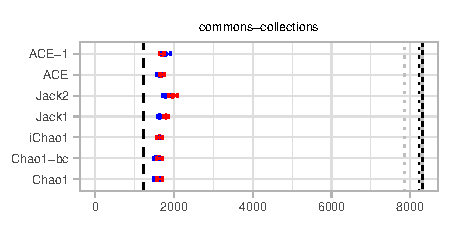
\includegraphics[width=0.9\linewidth]{charts_test/organic/commons-collections.pdf}
%        %\caption{1a}
%\end{subfigure}%
%\begin{subfigure}{.5\textwidth}
%    \centering
%      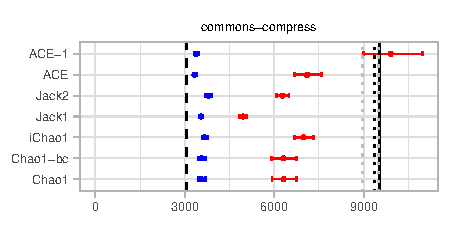
\includegraphics[width=0.9\linewidth]{charts_test/organic/commons-compress.pdf}
%        %\caption{1b}
%\end{subfigure}
%\begin{subfigure}{.5\textwidth}
%    \centering
%      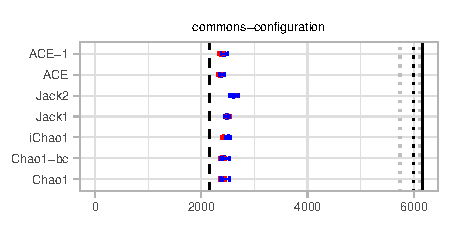
\includegraphics[width=0.9\linewidth]{charts_test/organic/commons-configuration.pdf}
%        %\caption{1b}
%\end{subfigure}%
%\begin{subfigure}{.5\textwidth}
%    \centering
%      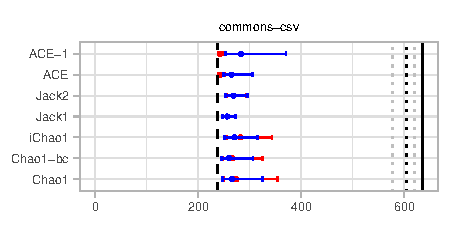
\includegraphics[width=0.9\linewidth]{charts_test/organic/commons-csv.pdf}
%        %\caption{1b}
%\end{subfigure}
%\begin{subfigure}{.5\textwidth}
%    \centering
%      \includegraphics[width=0.9\linewidth]{charts_test/organic/commons-dbcp.pdf}
%        %\caption{1b}
%\end{subfigure}%
%\begin{subfigure}{.5\textwidth}
%    \centering
%      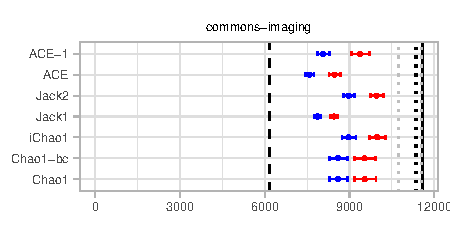
\includegraphics[width=0.9\linewidth]{charts_test/organic/commons-imaging.pdf}
%        %\caption{1b}
%\end{subfigure}
%\begin{subfigure}{.5\textwidth}
%    \centering
%      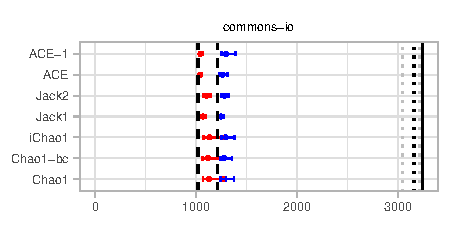
\includegraphics[width=0.9\linewidth]{charts_test/organic/commons-io.pdf}
%        %\caption{1b}
%\end{subfigure}%
%\begin{subfigure}{.5\textwidth}
%    \centering
%      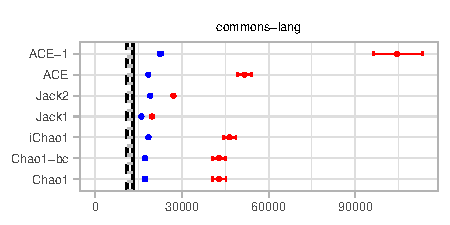
\includegraphics[width=0.9\linewidth]{charts_test/organic/commons-lang.pdf}
%        %\caption{1b}
%\end{subfigure}
%\begin{subfigure}{.5\textwidth}
%    \centering
%      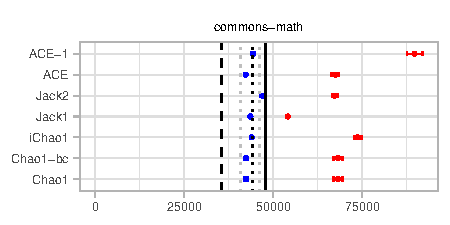
\includegraphics[width=0.9\linewidth]{charts_test/organic/commons-math.pdf}
%        %\caption{1b}
%\end{subfigure}%
%\begin{subfigure}{.5\textwidth}
%    \centering
%      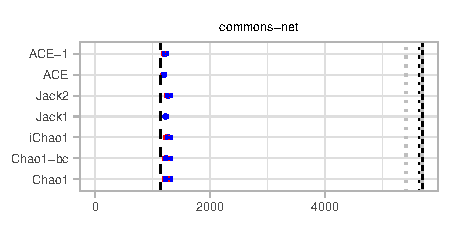
\includegraphics[width=0.9\linewidth]{charts_test/organic/commons-net.pdf}
%        %\caption{1b}
%\end{subfigure}
%  \caption{Estimators from test \original. The red is from \emph{class test set} data, and blue from \emph{method test set} data.}
%\label{fig:original}
%\end{figure*}

%
%
%\subsection{\EvosuiteRandom}
%\label{sec:random}
%\subsection{\EvosuiteStd}
%\label{sec:std}
%

%
%\subsection{Challenges Faced}
%During our empirical evaluation, we faced a number of challenges, and here is
%a list of some of the tougher challenges we faced.
%\begin{description}[leftmargin=0cm,labelindent=0cm]
%\item[Flacky tests.] Flaky tests were a major source of problems during our
%evaluation. In particular, tests that run and report no failure during manual
%runs sometimes fail during \PIT runs for extracting coverage.
%\item[Residual Errors in Classification.] We found that even after three fold confirmation,
%one of the mutants marked as equivalent was actually killed by an automatically
%generated test case.
%\item[\PIT bugs] The \PIT version we used sometimes resulted in corrupted XML
%files as output. Furthermore, \PIT would sometimes fail to detect bugs due to
%its incorrect coverage heuristics. We found that some such tests would detect
%mutants.
%\item[Sandboxes] When \PIT was used in programs that contained file IO, it
%often corrupted the file system, overwriting unintended files.
%\item[Bugs in R packages] Some of the statistical estimation packages had bugs
%in them, which we found thanks to implementing the estimation formulas
%ourselves and cross checking the results.
%\item[Limitations of \Evosuite] The \Evosuite test generator would not run on
%all programs we used.
%\end{description}
%

%\begin{figure*}
%\begin{subfigure}{.5\textwidth}
%    \centering
%      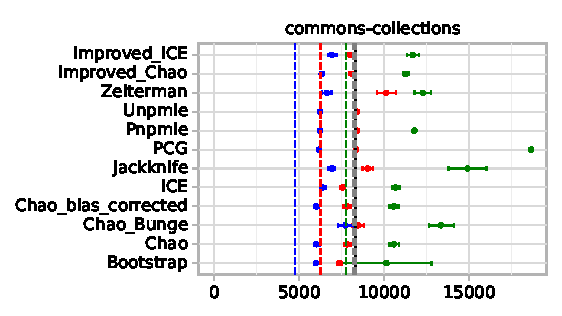
\includegraphics[width=0.9\linewidth]{charts/graph2/graph2/commons-collections.pdf}
%        %\caption{1a}
%\end{subfigure}%
%\begin{subfigure}{.5\textwidth}
%    \centering
%      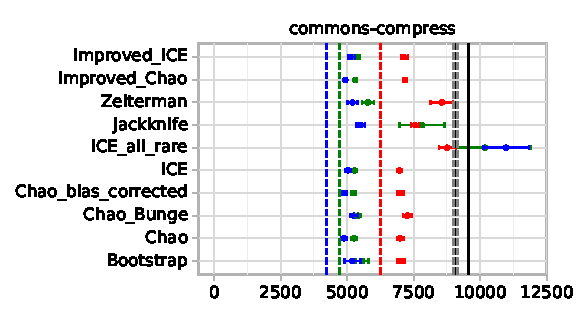
\includegraphics[width=0.9\linewidth]{charts/graph2/graph2/commons-compress.pdf}
%        %\caption{1b}
%\end{subfigure}
%\begin{subfigure}{.5\textwidth}
%    \centering
%      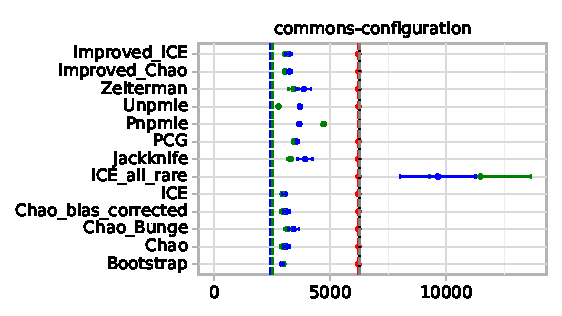
\includegraphics[width=0.9\linewidth]{charts/graph2/graph2/commons-configuration.pdf}
%        %\caption{1b}
%\end{subfigure}%
%\begin{subfigure}{.5\textwidth}
%    \centering
%      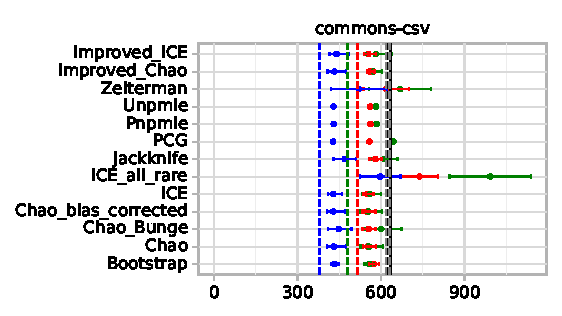
\includegraphics[width=0.9\linewidth]{charts/graph2/graph2/commons-csv.pdf}
%        %\caption{1b}
%\end{subfigure}
%\begin{subfigure}{.5\textwidth}
%    \centering
%      \includegraphics[width=0.9\linewidth]{charts/graph2/graph2/commons-dbcp.pdf}
%        %\caption{1b}
%\end{subfigure}%
%\begin{subfigure}{.5\textwidth}
%    \centering
%      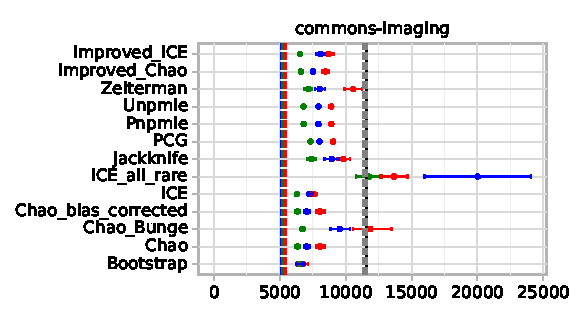
\includegraphics[width=0.9\linewidth]{charts/graph2/graph2/commons-imaging.pdf}
%        %\caption{1b}
%\end{subfigure}
%\begin{subfigure}{.5\textwidth}
%    \centering
%      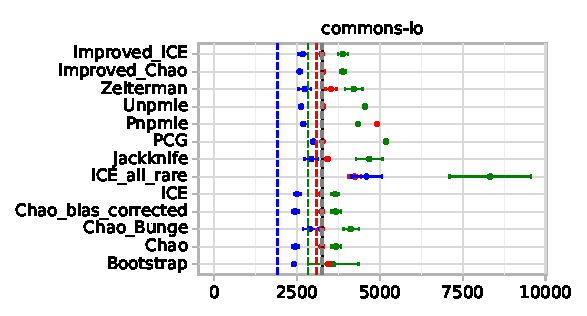
\includegraphics[width=0.9\linewidth]{charts/graph2/graph2/commons-io.pdf}
%        %\caption{1b}
%\end{subfigure}%
%\begin{subfigure}{.5\textwidth}
%    \centering
%      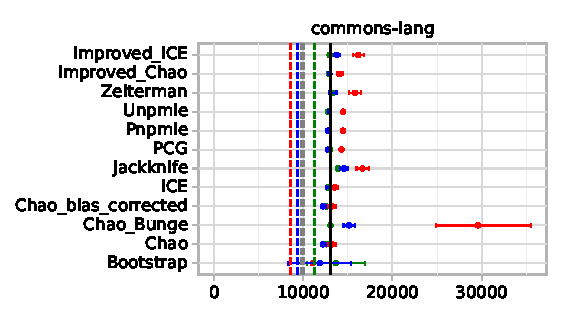
\includegraphics[width=0.9\linewidth]{charts/graph2/graph2/commons-lang.pdf}
%        %\caption{1b}
%\end{subfigure}
%\begin{subfigure}{.5\textwidth}
%    \centering
%      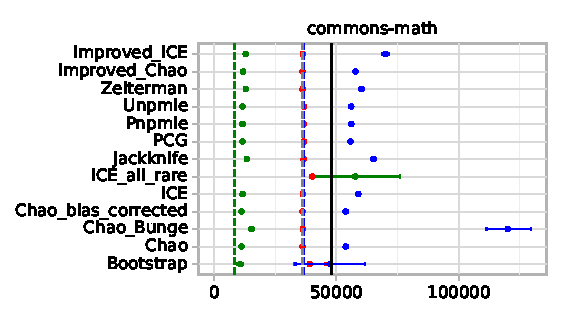
\includegraphics[width=0.9\linewidth]{charts/graph2/graph2/commons-math.pdf}
%        %\caption{1b}
%\end{subfigure}%
%\begin{subfigure}{.5\textwidth}
%    \centering
%      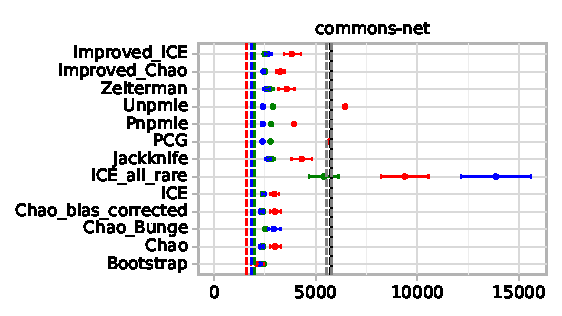
\includegraphics[width=0.9\linewidth]{charts/graph2/graph2/commons-net.pdf}
%        %\caption{1b}
%\end{subfigure}
%  \caption{method test data, with test suites indicated by color.
%  \original is \textcolor{red}{red}, \EvosuiteRandom is \textcolor{blue}{blue}
%  and \EvosuiteDynamosa is \textcolor{green}{green}.
%  Dashed lines represent killed mutants by respective test cases,
%  and error bars represent estimates from
%  mutant kills by each estimator. The solid black line is the total mutants
%  generated, dashed black line the manual estimate, and gray dashed lines the
%  error bars.}
%\label{fig:testmethods}
%\end{figure*}
%
%
%\begin{figure*}
%\begin{subfigure}{\textwidth}
%    \centering
%      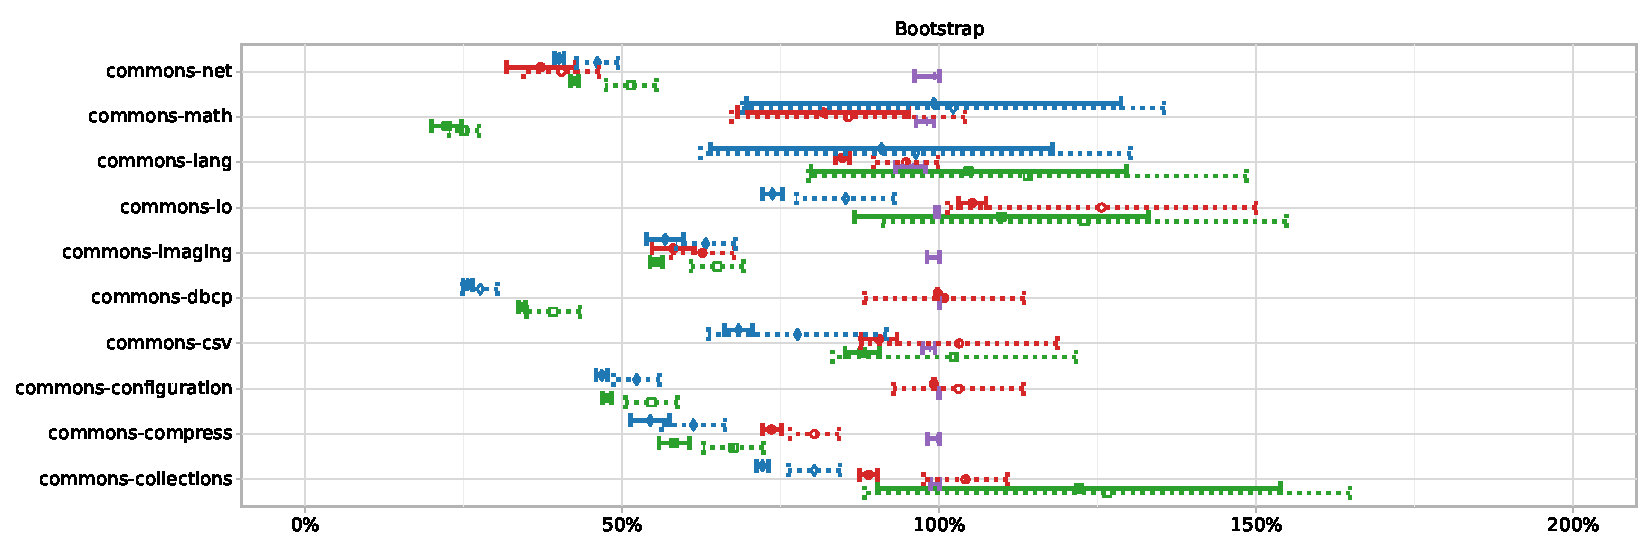
\includegraphics[width=0.9\linewidth]{estimators/Bootstrap.pdf}
%        %\caption{1a}
%\end{subfigure}
%\begin{subfigure}{\textwidth}
%    \centering
%      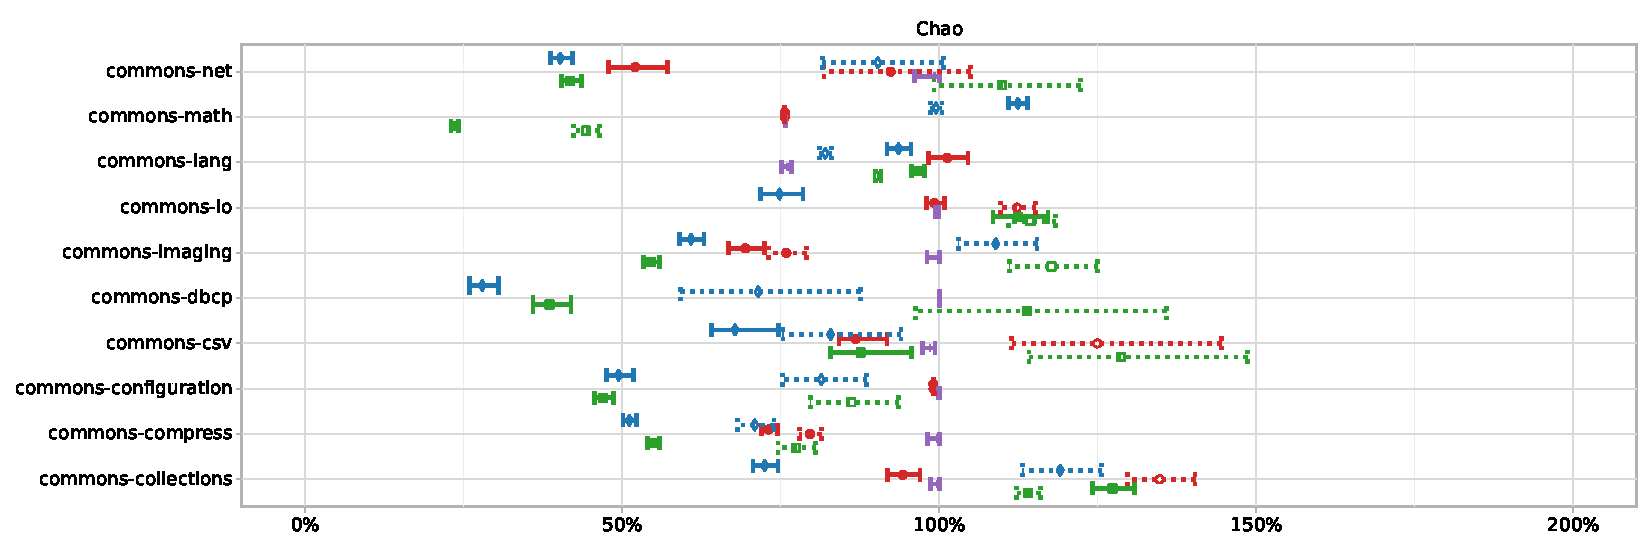
\includegraphics[width=0.9\linewidth]{estimators/Chao.pdf}
%        %\caption{1b}
%\end{subfigure}
%\begin{subfigure}{\textwidth}
%    \centering
%      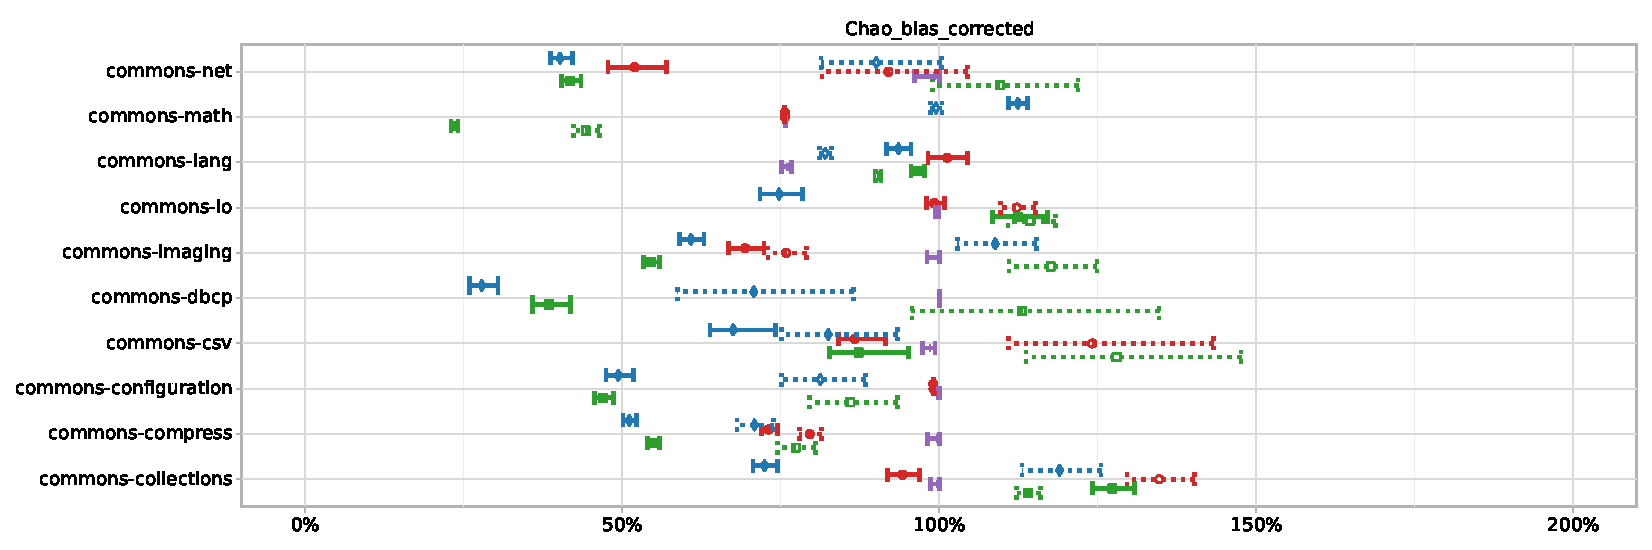
\includegraphics[width=0.9\linewidth]{estimators/Chao_bias_corrected.pdf}
%        %\caption{1b}
%\end{subfigure}
%\begin{subfigure}{\textwidth}
%    \centering
%      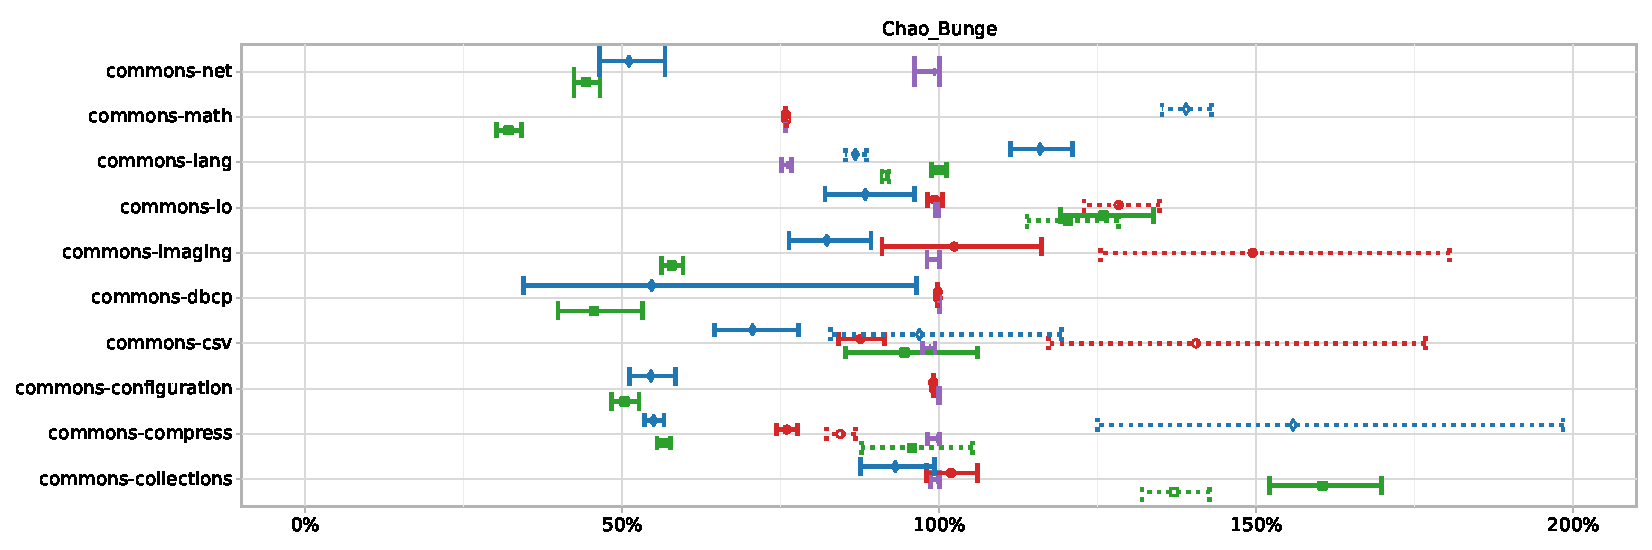
\includegraphics[width=0.9\linewidth]{estimators/Chao_Bunge.pdf}
%        %\caption{1b}
%\end{subfigure}
%  \caption{test data, with test suites indicated by color.
%  The manual classification is in \textcolor{purple}{purple}.
%  \original is \textcolor{red}{red}, \EvosuiteRandom is \textcolor{blue}{blue}
%  and \EvosuiteDynamosa is \textcolor{green}{green}.
%  Dashed lines represent estimates and errorbars from class based samples
%  while solid lines represent estimates and errorbars from method based
%  samples.
% } 
%\label{fig:estimates}
%\end{figure*}
%
%
%\begin{figure*}
%\begin{subfigure}{\textwidth}
%    \centering
%      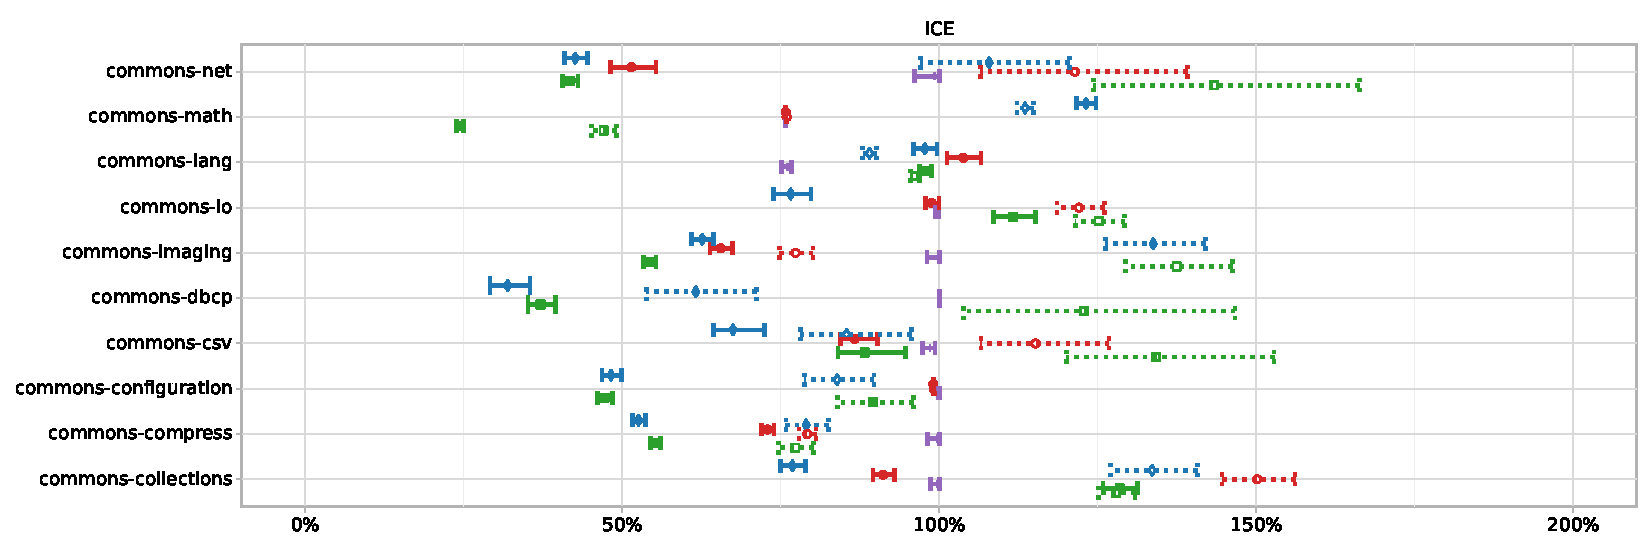
\includegraphics[width=0.9\linewidth]{estimators/ICE.pdf}
%        %\caption{1b}
%\end{subfigure}
%\begin{subfigure}{\textwidth}
%    \centering
%      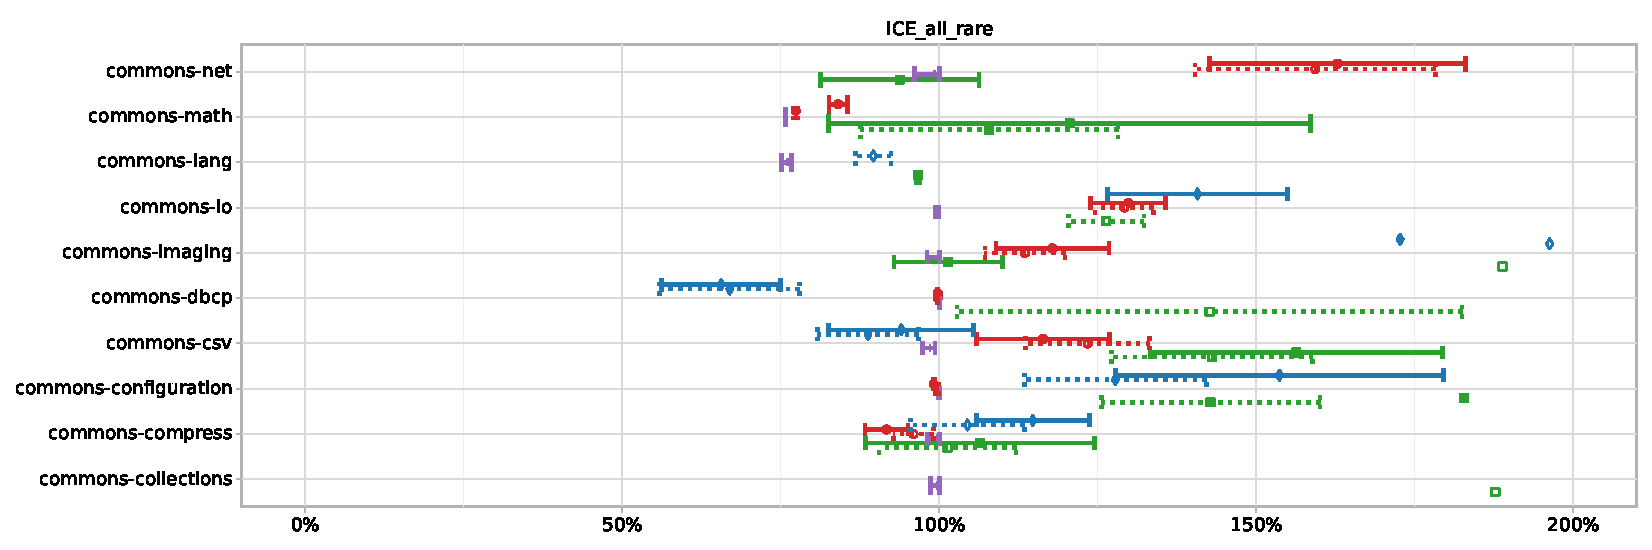
\includegraphics[width=0.9\linewidth]{estimators/ICE_all_rare.pdf}
%        %\caption{1b}
%\end{subfigure}
%\begin{subfigure}{\textwidth}
%    \centering
%      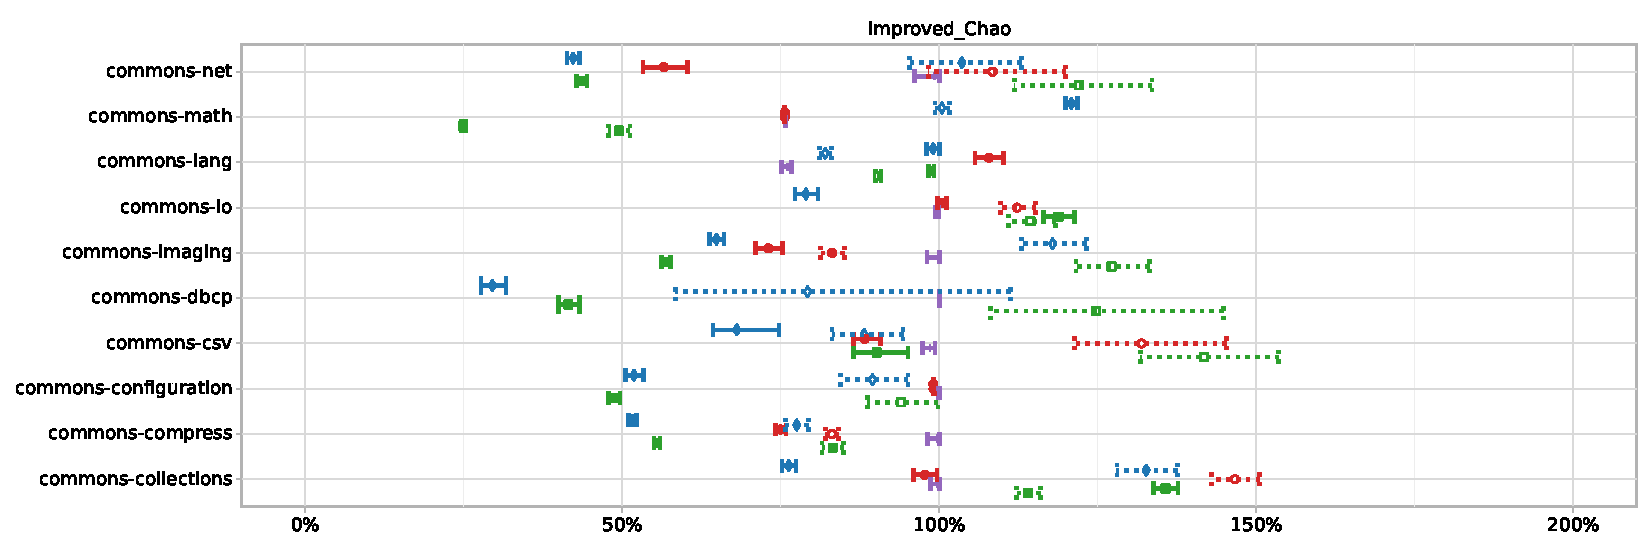
\includegraphics[width=0.9\linewidth]{estimators/improved_Chao.pdf}
%        %\caption{1b}
%\end{subfigure}
%\begin{subfigure}{\textwidth}
%    \centering
%      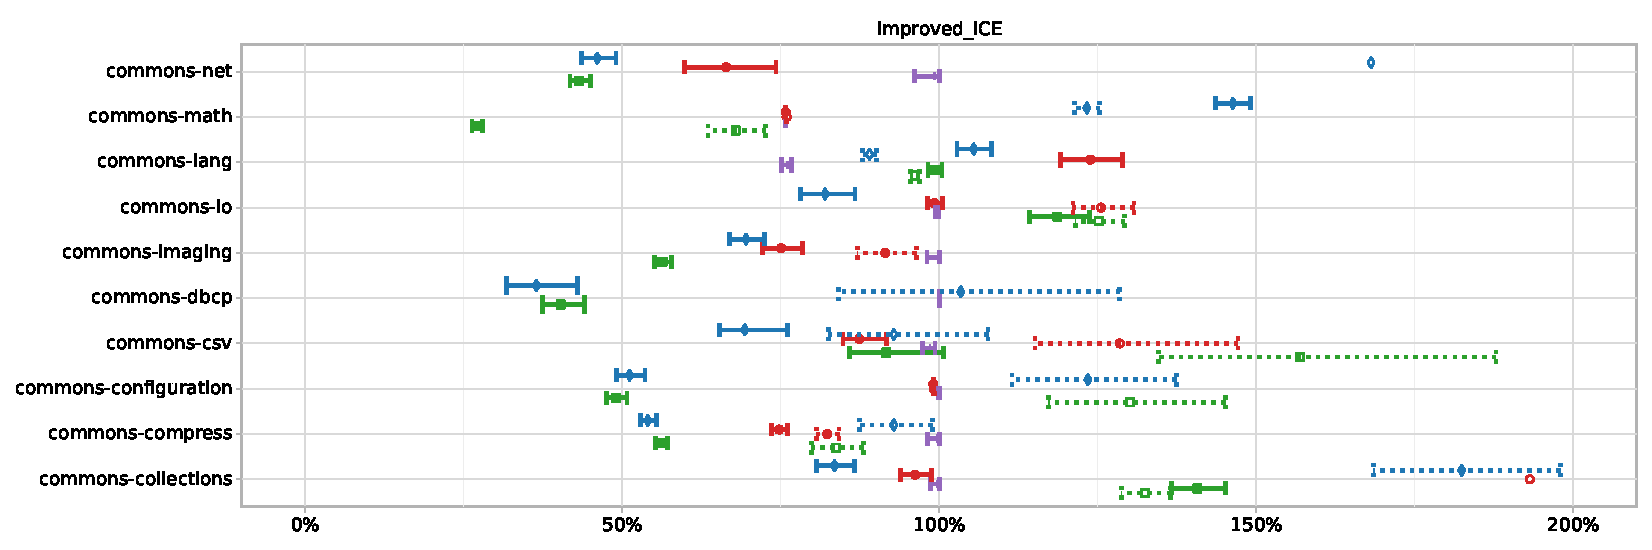
\includegraphics[width=0.9\linewidth]{estimators/improved_ICE.pdf}
%        %\caption{1b}
%\end{subfigure}
%% \begin{subfigure}{\textwidth}
%%     \centering
%%       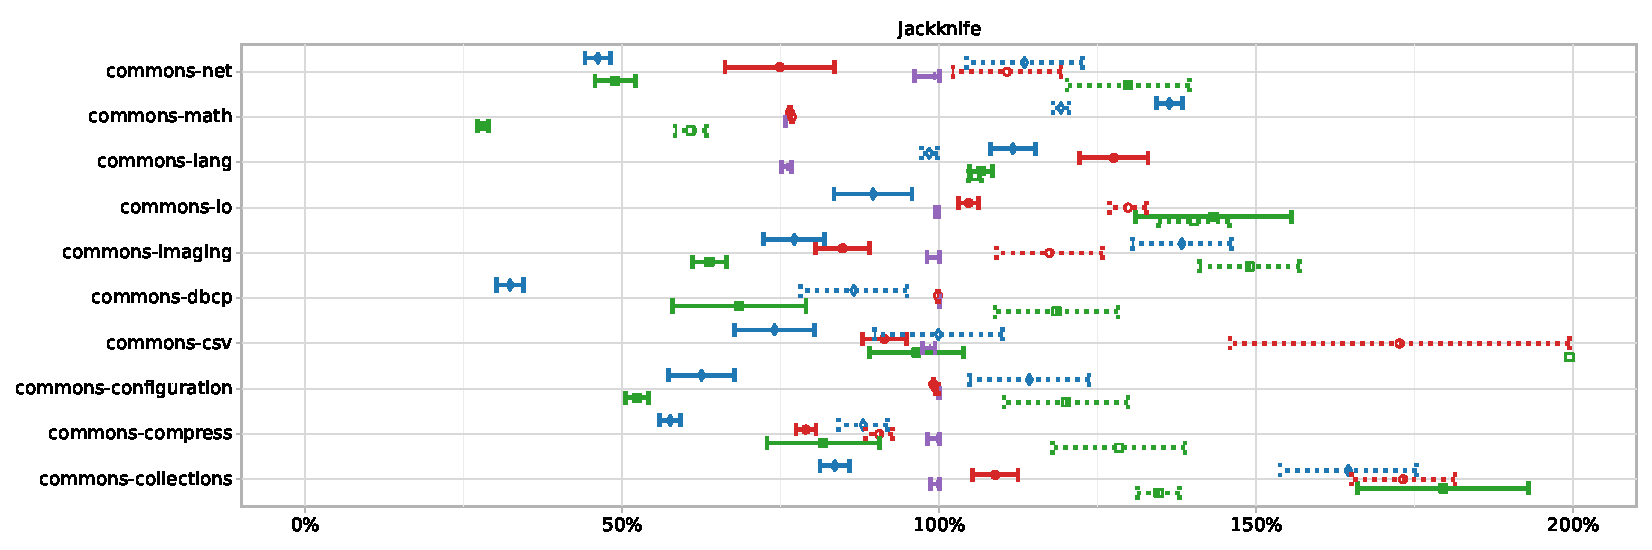
\includegraphics[width=0.9\linewidth]{estimators/Jackknife.pdf}
%%         %\caption{1b}
%% \end{subfigure}
%% \begin{subfigure}{\textwidth}
%%     \centering
%%       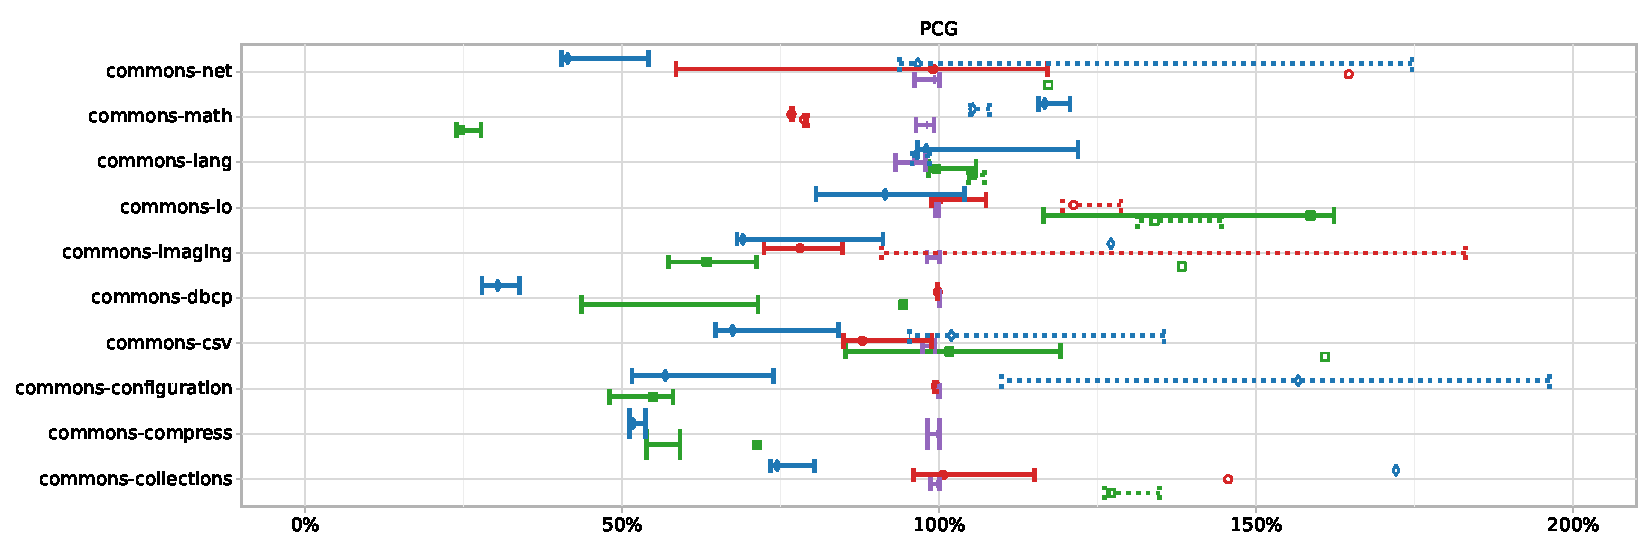
\includegraphics[width=0.9\linewidth]{estimators/PCG.pdf}
%%         %\caption{1b}
%% \end{subfigure}
%  \caption{test data, with test suites indicated by color.
%  The manual classification is in \textcolor{purple}{purple}.
%  \original is \textcolor{red}{red}, \EvosuiteRandom is \textcolor{blue}{blue}
%  and \EvosuiteDynamosa is \textcolor{green}{green}.
%  Dashed lines represent estimates and errorbars from class based samples
%  while solid lines represent estimates and errorbars from method based
%  samples.
% } 
%\label{fig:estimates2}
%\end{figure*}
%
%\begin{figure*}
%\begin{subfigure}{\textwidth}
%    \centering
%      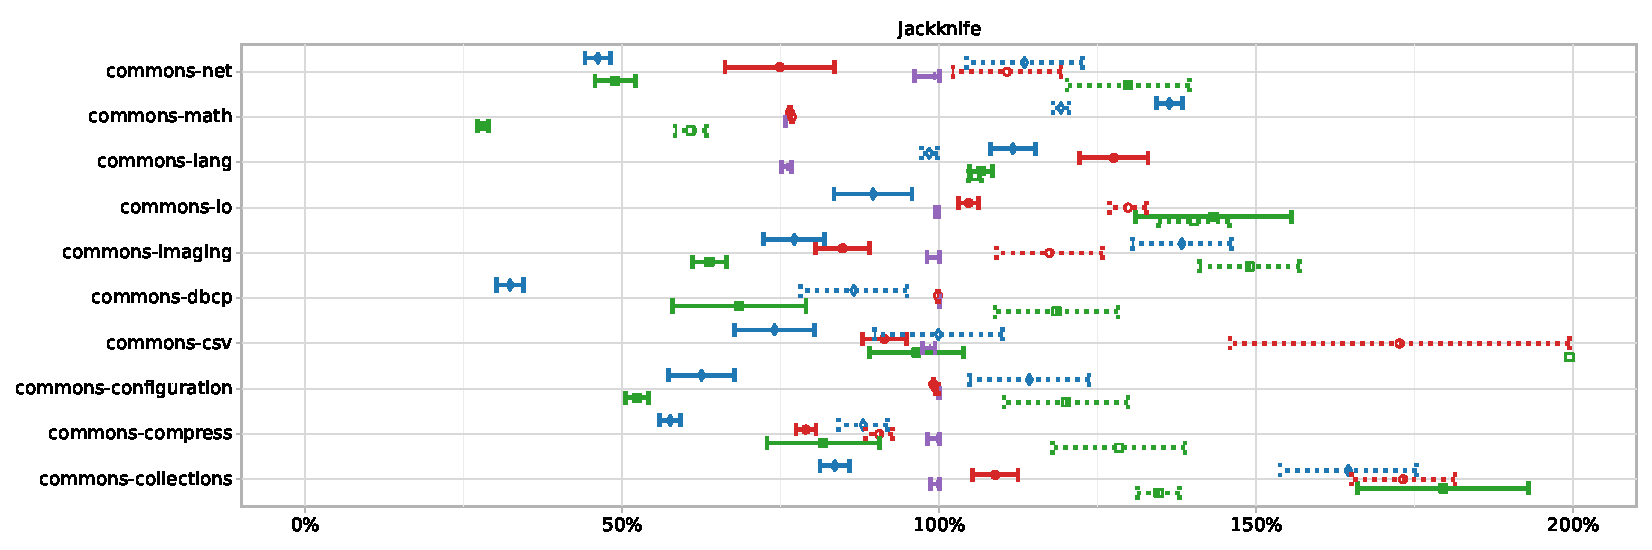
\includegraphics[width=0.9\linewidth]{estimators/Jackknife.pdf}
%        %\caption{1b}
%\end{subfigure}
%\begin{subfigure}{\textwidth}
%    \centering
%      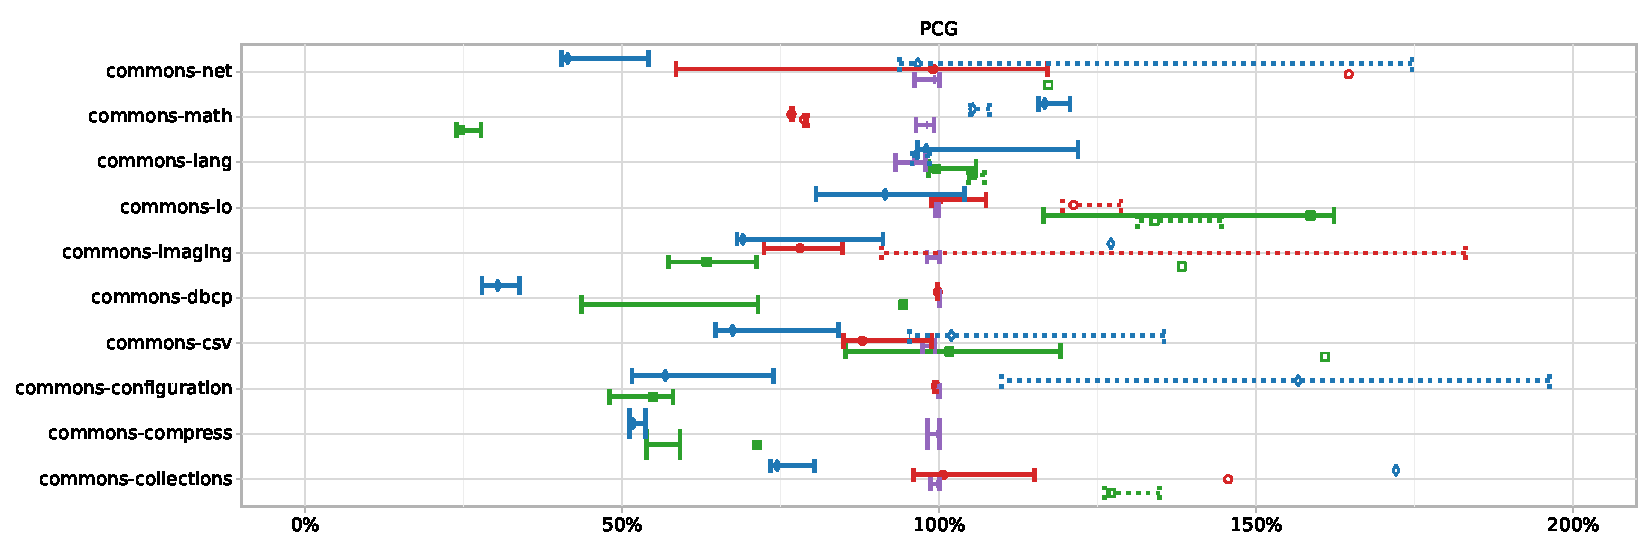
\includegraphics[width=0.9\linewidth]{estimators/PCG.pdf}
%        %\caption{1b}
%\end{subfigure}
%\begin{subfigure}{\textwidth}
%    \centering
%      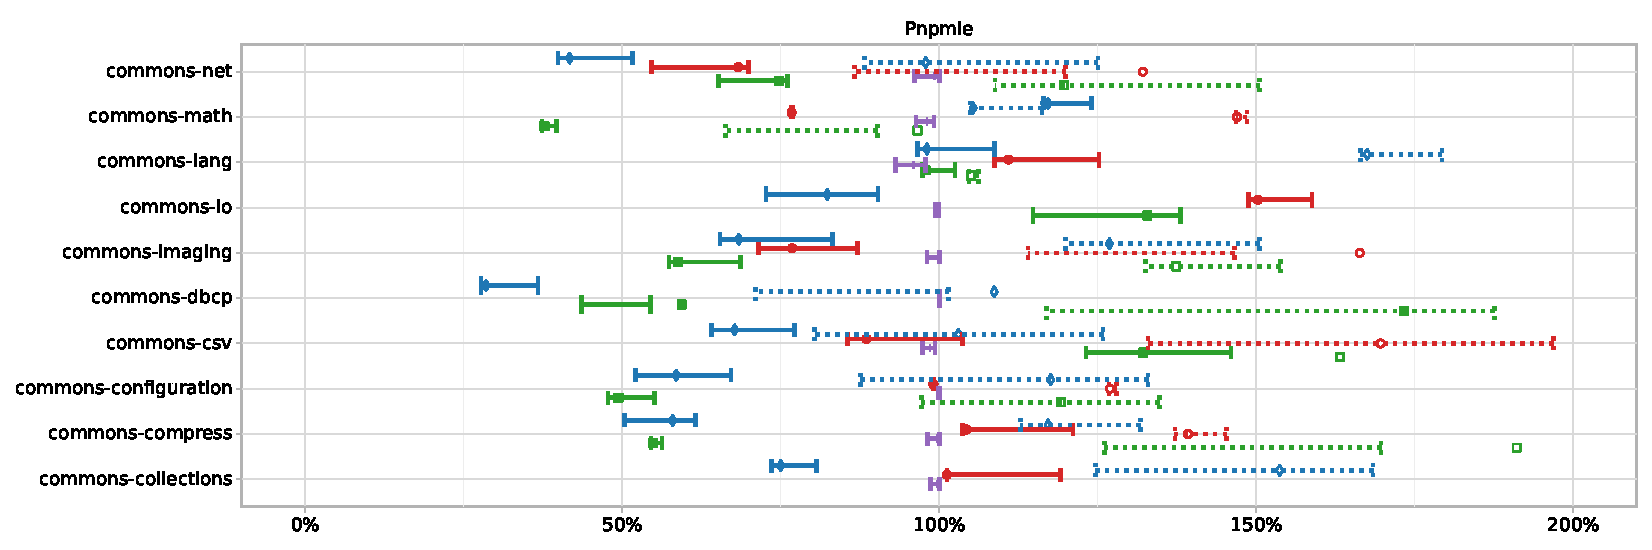
\includegraphics[width=0.9\linewidth]{estimators/Pnpmle.pdf}
%        %\caption{1b}
%\end{subfigure}
%\begin{subfigure}{\textwidth}
%    \centering
%      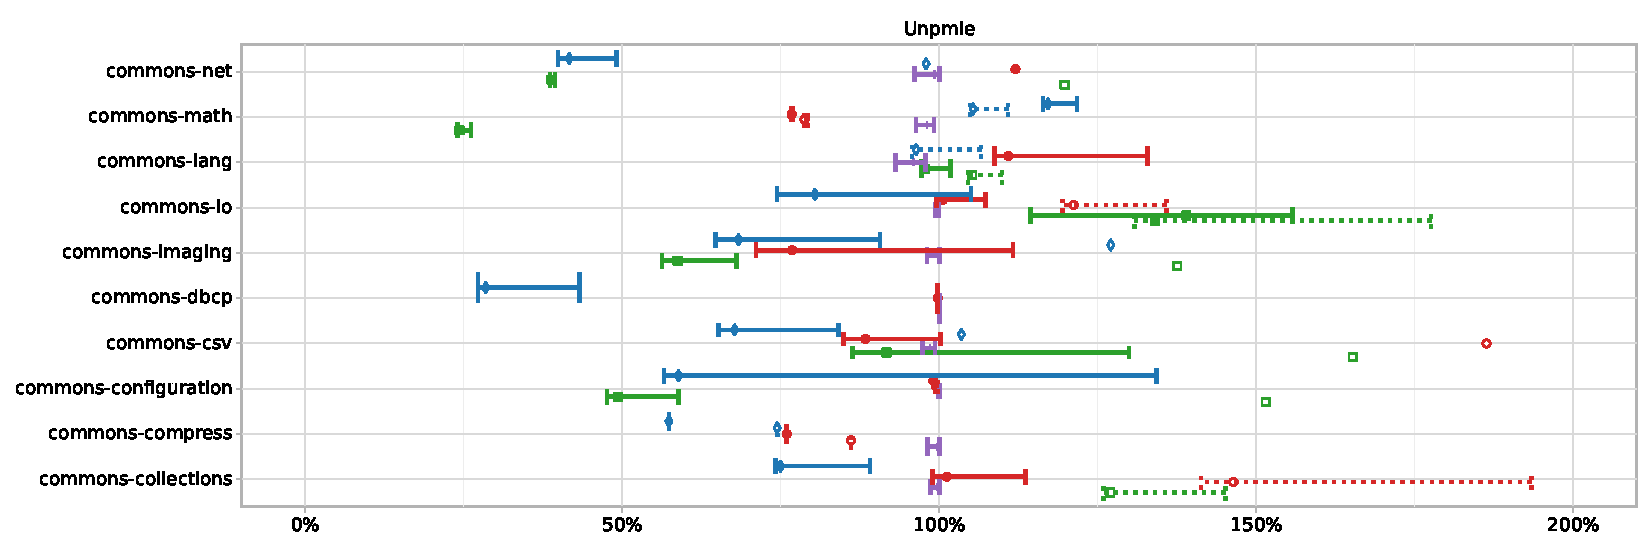
\includegraphics[width=0.9\linewidth]{estimators/Unpmle.pdf}
%        %\caption{1b}
%\end{subfigure}
%%\begin{subfigure}{\textwidth}
%%    \centering
%%      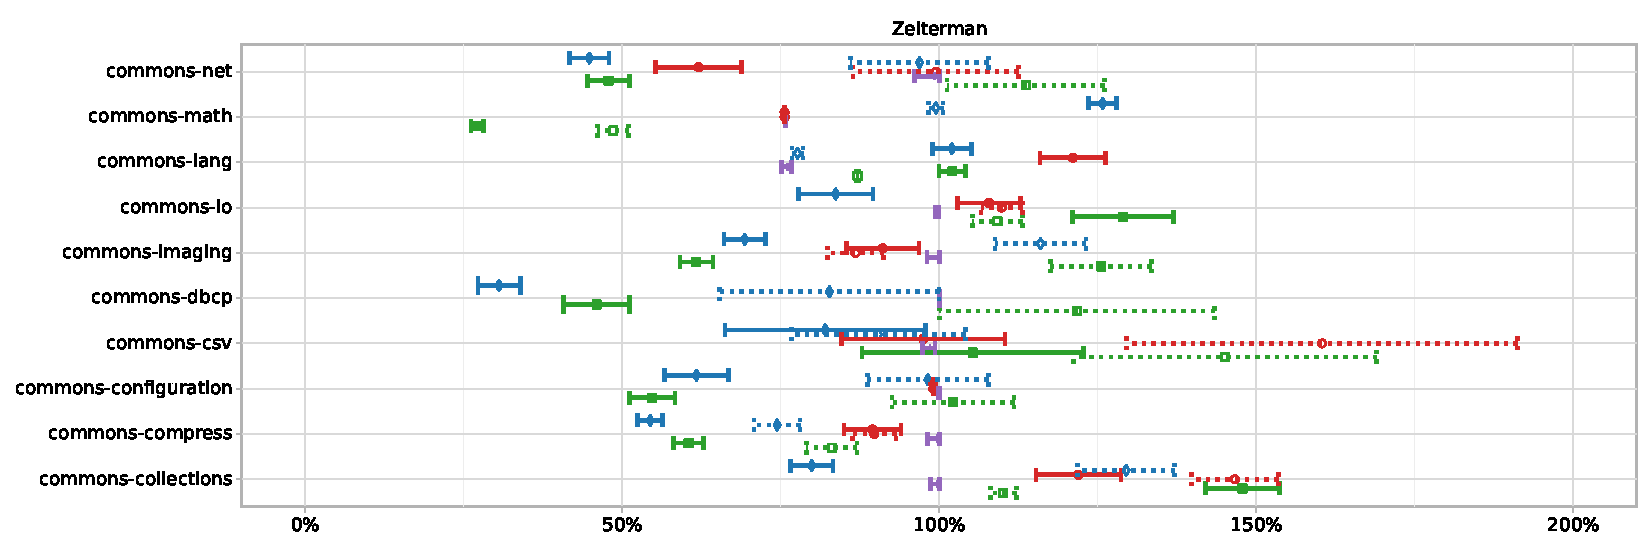
\includegraphics[width=0.9\linewidth]{estimators/Zelterman.pdf}
%%        %\caption{1b}
%%\end{subfigure}
%  \caption{test data, with test suites indicated by color.
%  The manual classification is in \textcolor{purple}{purple}.
%  \original is \textcolor{red}{red}, \EvosuiteRandom is \textcolor{blue}{blue}
%  and \EvosuiteDynamosa is \textcolor{green}{green}.
%  Dashed lines represent estimates and errorbars from class based samples
%  while solid lines represent estimates and errorbars from method based
%  samples.
% } 
%\label{fig:estimates3}
%\end{figure*}
%\begin{figure*}
%\begin{subfigure}{\textwidth}
%    \centering
%      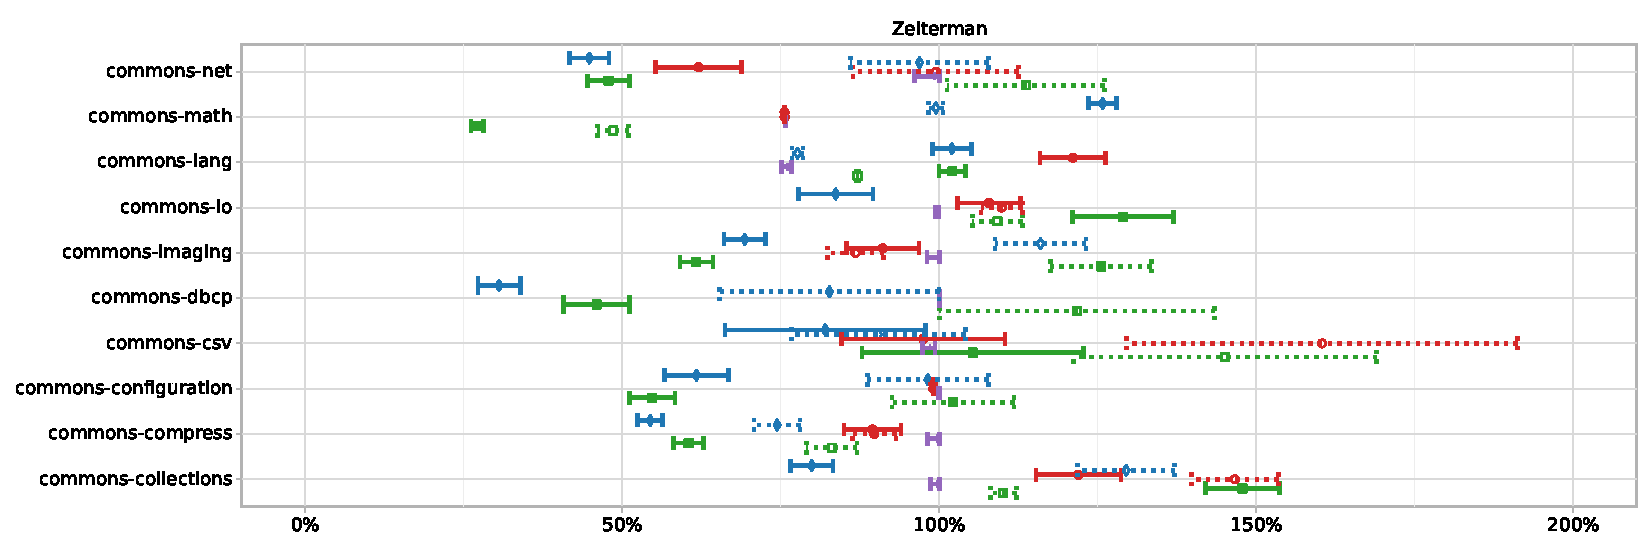
\includegraphics[width=0.9\linewidth]{estimators/Zelterman.pdf}
%        %\caption{1b}
%\end{subfigure}
%  \caption{test data, with test suites indicated by color.
%  The manual classification is in \textcolor{purple}{purple}.
%  \original is \textcolor{red}{red}, \EvosuiteRandom is \textcolor{blue}{blue}
%  and \EvosuiteDynamosa is \textcolor{green}{green}.
%  Dashed lines represent estimates and errorbars from class based samples
%  while solid lines represent estimates and errorbars from method based
%  samples.
% } 
%\label{fig:estimates4}
%\end{figure*}

%\maketitle
\end{document}
\endinput
